% =====================================================================
%  CLD 880 - Minor Project Report
%  Sakhare Yash Balram, 2022CH71496
%  Department of Chemical Engineering, IIT Delhi
%
%  Single-column journal-style layout based on the article class so the
%  file compiles without an external journal class.  Body text is
%  one-and-a-half-spaced; section headings are sans-serif numbered in
%  the IJHE style we follow throughout the project.
% =====================================================================

\documentclass[11pt,a4paper]{article}

% - core typesetting -
\usepackage[T1]{fontenc}
\usepackage{lmodern}
\usepackage[utf8]{inputenc}
\usepackage{microtype}
\DisableLigatures[-]{encoding = T1, family = *}
\usepackage[english]{babel}
\usepackage{geometry}
\geometry{a4paper,top=25mm,bottom=25mm,left=25mm,right=25mm}
\usepackage{setspace}
\onehalfspacing

% - math & units -
\usepackage{amsmath}
\usepackage{amssymb}
\usepackage{siunitx}
\sisetup{detect-all,per-mode=symbol}

% - figures, tables, captions -
\usepackage{graphicx}
\usepackage{float}
\usepackage{subcaption}
\usepackage{booktabs}
\usepackage[font=small,labelfont=bf,labelsep=period]{caption}

% - section headings (journal-ish look) -
\usepackage[explicit]{titlesec}
\titleformat{\section}{\sffamily\large\bfseries}{\thesection.}{0.5em}{#1}
\titleformat{\subsection}{\sffamily\normalsize\bfseries}{\thesubsection.}{0.5em}{#1}
\titleformat{\subsubsection}{\sffamily\normalsize\itshape}{\thesubsubsection.}{0.5em}{#1}
\titleformat{\paragraph}[runin]{\sffamily\normalsize\bfseries}{}{0pt}{#1}

% - bibliography -
\usepackage[numbers,sort&compress,square]{natbib}

% - hyperlinks (kept boring on purpose) -
\usepackage[hidelinks,unicode=true,psdextra=true]{hyperref}
\pdfstringdefDisableCommands{%
  \def\Hi{H2}%
  \def\CHi{CH4}%
  \def\dD{d/D}%
  \def\VR{VR}%
  \def\HBR{HBR}%
  \def\CoV{CoV}%
  \def\Ri{Ri}%
  \def\Frnum{Fr}%
  \def\^#1{#1}%
  \def\circ{ deg}%
}

% - helpers -
\usepackage{xcolor}
\newcommand{\Hi}{\ensuremath{\mathrm{H_2}}}
\newcommand{\CHi}{\ensuremath{\mathrm{CH_4}}}
\newcommand{\dD}{\ensuremath{d/D}}
\newcommand{\VR}{\ensuremath{\mathrm{VR}}}
\newcommand{\HBR}{\ensuremath{\mathrm{HBR}}}
\newcommand{\CoV}{\ensuremath{\mathrm{CoV}}}
\newcommand{\Ri}{\ensuremath{\mathrm{Ri}}}
\newcommand{\Frnum}{\ensuremath{\mathrm{Fr}}}

\title{}
\author{}
\date{}

\begin{document}

% =====================================================================
%  TITLE / COVER PAGE  (everything on a single page)
% =====================================================================
\begin{titlepage}
    \centering
    \vspace*{0.4cm}
    {\large \bfseries Minor Project Report \par}
    \vspace{0.15cm}
    {\large \bfseries CLD\,880 \par}
    \vspace{1.2cm}

    {\LARGE \bfseries Multiobjective Optimization of \\[0.15cm]
    Hydrogen Injection into High-Pressure \\[0.15cm]
    Natural Gas Pipelines \par}

    \vspace{0.5cm}
    {\large \bfseries A Surrogate-Assisted Multi-Objective Approach \par}

    \vspace{1.2cm}
    {\large Submitted by \par}
    \vspace{0.25cm}
    {\Large \bfseries Sakhare Yash Balram \par}
    {\large 2022CH71496 \par}

    \vspace{0.7cm}
    {\large Under the supervision of \par}
    \vspace{0.25cm}
    {\Large \bfseries Prof.~Abhijeet Raj \par}

    \vspace{1.0cm}
    \IfFileExists{logos/IITD_Logo_Big.jpg}{%
        
\includegraphics[width=0.22\textwidth]{logos/IITD_Logo_Big.jpg}%
    }{%
        \IfFileExists{logos/IITD_Logo_Big.png}{%
            
\includegraphics[width=0.22\textwidth]{logos/IITD_Logo_Big.png}%
        }{%
            \fbox{\parbox[c][2.6cm][c]{0.32\textwidth}{\centering\itshape\footnotesize
                drop IITD logo file in \texttt{logos/}}}%
        }%
    }\par
    \vspace{0.6cm}

    {\large \bfseries Department of Chemical Engineering \par}
    {\large \bfseries Indian Institute of Technology Delhi \par}
    {\large \bfseries New Delhi - 110016 \par}
    \vspace{0.25cm}
    {\large \bfseries April 2026 \par}

    \vfill
    \renewcommand{\arraystretch}{1.4}
    \begin{tabular}{|p{0.42\textwidth}|p{0.42\textwidth}|}
        \hline
        \centering \textbf{Supervisor's signature} &
        \centering \textbf{Date} \tabularnewline
        \hline
        \vspace{1.2cm} & \vspace{1.2cm} \tabularnewline
        \hline
    \end{tabular}
    \vspace*{0.2cm}
\end{titlepage}

% =====================================================================
%  ABSTRACT
% =====================================================================
\begin{center}
    {\Large \bfseries \sffamily Abstract}
\end{center}
\noindent
Blending green hydrogen into existing natural-gas networks (HBNG) is
a practical short-term route to decarbonising the gas grid without
rebuilding it. The challenge is physical: hydrogen is roughly eight
times lighter than methane, so the two gases stratify rather than
mix uniformly, and incomplete mixing exposes the pipe wall to
near-pure hydrogen, biases custody-transfer metering and broadens the
flammability envelope at end-burners. This work presents a CFD-based
parametric study of \Hi{} injection through a side branch into a
\(\SI{0.46}{\meter}\) methane main pipe carrying gas at
\(\SI{10}{\meter\per\second}\), using the compressible buoyant solver
\texttt{rhoReactingBuoyantFoam} in OpenFOAM with the
\(k\)-\(\omega\)~SST turbulence closure. Three independent design variables
are swept: the diameter ratio \(\dD\in[0.15,\,0.45]\), the velocity
ratio \(\VR=u_{\mathrm{branch}}/u_{\mathrm{main}}\in[0.69,\,5.84]\),
and the injection angle \(\alpha\in\{30^\circ,\,90^\circ\}\). The
hydrogen blending ratio \(\HBR\) is \emph{not} an independent
fourth knob; once \((\dD,\VR)\) are fixed, \(\HBR\) follows from a
volumetric-flow balance and lies in \([0.06,\,0.20]\) across the
design. Two ten-case sliced Latin Hypercube campaigns share the
same \((\dD,\VR)\) seed, one at each angle, so seven
matched-parameter pairs let the angle effect be cleanly isolated
from the LHS scatter while each campaign on its own resolves the
within-angle (\dD,~\VR) trends. Mixing quality is reported
as the coefficient of variation \CoV{} of the outlet \Hi{}
mass-fraction, and pumping cost as the low-pass-filtered
inlet-outlet gauge pressure drop
\(|\Delta p_{\mathrm{rgh}}|\); the LP filter is necessary because
the compressible solver carries
\(\mathcal{O}(25\,\si{\kilo\pascal})\) acoustic ringing on top of
the \(\mathcal{O}(1\!-\!3\,\si{\kilo\pascal})\) flow-loss signal,
as discussed in Section~\ref{sec:dp_filter}. The paired comparison
gives a clear and quantitative result: at every matched operating
point, the \(30^\circ\) tilt mixes better than the \(90^\circ\) T
(median \CoV{} reduction of \(46\,\%\)), and in all seven pairs it
also costs less to pump (median \(|\Delta p|\) reduction of
\(63\,\%\)). A power-law fit gives \(\CoV \sim \VR^{-1.16}\) at
\(90^\circ\) and \(\sim \VR^{-1.88}\) at \(30^\circ\)
(\(R^2_{\log} = 0.80\) at both angles), so the tilted geometry
converts each unit of velocity ratio into more mixing. The physical
mechanism, evident in side-by-side centreline contours, is that the
perpendicular jet impinges on the opposite wall and locks the
hydrogen into a wall-attached tongue, while the tilted jet feeds a
streamwise shear layer and a long under-junction recirculation that
homogenise the cross-section by the time the flow reaches the
outlet. The non-dimensional junction loss coefficient
\(K = |\Delta p|/q_{\mathrm{dyn,main}}\) lands in the classical
unshaped-T handbook range (median \(K_{90^\circ}\!\approx 0.78\)) and
is uniformly lower at \(30^\circ\) (median \(K_{30^\circ}\!\approx
0.26\)), in agreement with the Idelchik tee-junction tabulations.
The combined Pareto front therefore shifts down-and-left with
tilt: case~01 of the \(30^\circ\) campaign reaches \(\CoV = 0.5\,\%\)
at \(|\Delta p|\!\approx\SI{4.2}{\kilo\pascal}\), and case~09 of
the \(30^\circ\) campaign provides cheap pumping
(\(\SI{0.3}{\kilo\pascal}\)) with modest mixing - both points
dominate every \(90^\circ\) design in the database. The practical
recommendation that follows is to prefer a moderately tilted branch
wherever the layout permits, since it relaxes both halves of the
mixing-vs-pumping trade-off simultaneously. The surrogate model
and NSGA-II multi-objective optimiser that sit downstream of this
CFD dataset were prototyped on the \(90^\circ\) campaign at the
mid-semester review of the Minor Project; the only remaining
work, namely closing the angle axis with the queued
fixed-(\dD,\VR) campaign(s) on the newly-secured large-compute
allocation and re-fitting the surrogate on the merged dataset,
is scheduled for completion before the end-semester
presentation. All simulation case templates, mesh tools,
post-processing scripts and figure code used in this report are
open-source on GitHub (\url{https://github.com/Yash04dsr/MTP-Work};
full reproduction notes in Section~\ref{sec:data_avail}).

\vspace{1em}
\noindent
\textbf{Keywords:} hydrogen blending; natural gas; T-junction; CFD;
RANS; \(k\)-\(\omega\)~SST; OpenFOAM; Latin Hypercube Sampling;
coefficient of variation; injection angle; velocity ratio;
diameter ratio.

\clearpage

% =====================================================================
%  CONTENTS
% =====================================================================
\tableofcontents
\clearpage

% =====================================================================
%  1. INTRODUCTION
% =====================================================================
\section{Introduction}
\label{sec:intro}

\subsection{Why hydrogen-blended natural gas (HBNG)}
The push to decarbonise the energy system is constrained by an
awkward economic fact: building a parallel hydrogen pipeline grid
from scratch is far too expensive to do quickly. India's natural-gas
grid alone runs to several thousand kilometres of high-pressure steel
pipe that has already been paid for. Reusing that asset by blending
hydrogen into the existing methane stream - known as
Hydrogen-Blended Natural Gas (HBNG) - is the standard transition
strategy proposed in the recent literature
\citep{su2022prediction,arya2023multi,montanes2024comprehensive}.
The same pipeline can also serve as a ``chemical battery'' for
surplus solar and wind generation through the Power-to-Gas (P2G)
route, converting curtailed electricity into hydrogen and storing it
in a network the size of an existing gas grid \citep{arya2023multi}.
Recent techno-economic assessments by the National Renewable Energy
Laboratory \citep{topolski2022blending} indicate that a blend of up to
\(20\,\%\) hydrogen by volume is generally compatible with existing
steel infrastructure, although operating cost rises non-linearly
because hydrogen carries only about a third of the volumetric energy
density of methane.

\subsection{The mixing problem}
\label{sec:intro_mixing}
Hydrogen and methane have very different physical properties
(Table~\ref{tab:properties}). The eight-to-one density ratio is the
dominant practical issue: in a horizontal pipe at low velocity the
lighter \Hi{} floats up and forms a layer along the crown of the
pipe instead of mixing into the methane stream below. Three
downstream consequences follow.
\begin{enumerate}
    \item \textbf{Hydrogen embrittlement of the pipe wall.}\;
    The rate of hydrogen-induced cracking in pipe steels (notably
    grade X70) scales like \(p_{\Hi}^{0.5}\), so even a nominally
    \(10\,\%\) blend can expose the pipe crown to nearly pure
    hydrogen if stratification persists \citep{topolski2022blending}.
    \item \textbf{Combustion instability at end-burners.}\;
    The Wobbe Index, \(I_W = V_c/\sqrt{G}\), drifts when the burner
    sees fluctuating composition; hydrogen's wider flammability range
    (4-76\,\% vs. 5-15\,\% for methane) and roughly six-fold higher
    laminar flame speed make flashback a real risk
    \citep{topolski2022blending}.
    \item \textbf{Metering error.}\;
    Ultrasonic flow meters infer composition from the speed of sound;
    the gap between \(\sim\SI{1300}{\meter\per\second}\) in hydrogen
    and \(\sim\SI{450}{\meter\per\second}\) in methane is large
    enough that a stratified flow produces custody-transfer-grade
    composition errors \citep{su2022prediction}.
\end{enumerate}

\begin{table}[H]
\centering
\small
\caption{Selected physical properties of \Hi{} and \CHi{} at standard
temperature and pressure, and their consequence for T-junction
injection \citep{su2022prediction,montanes2024comprehensive}.}
\label{tab:properties}
\begin{tabular}{lccl}
\toprule
\textbf{Property} & \textbf{\CHi{}} & \textbf{\Hi{}} & \textbf{Consequence} \\
\midrule
Density (\si{\kg\per\cubic\metre})       & 0.668 & 0.082 & \(8\times\) density gap; stratification risk \\
Molecular weight (\si{\g\per\mol})        & 16.04 & 2.016 & low momentum per kg of fuel \\
Dynamic viscosity (\(10^{-6}\,\si{\pascal\second}\)) & 11.07 & 8.41 & shifts \(Re\) at fixed \(u\) \\
Mass diffusivity (\si{\square\centi\metre\per\second}) & low & 0.61 & turbulence dominates over molecular \\
Volumetric energy (\si{\mega\joule\per\cubic\metre}) & 36 & 11 & \(\sim\!3\times\) flow needed for same energy \\
Flammability range (vol \%)               & 5-15 & 4-76 & wider explosion envelope \\
\bottomrule
\end{tabular}
\end{table}

\subsection{Where the injection angle fits in}
There is by now a sizeable CFD literature on T-junction blending,
but most parametric studies fix the branch angle at
\(\alpha=90^\circ\) (perpendicular cross-flow) and sweep the
diameter ratio \(\dD\), the velocity ratio
\(\VR=u_{\mathrm{branch}}/u_{\mathrm{main}}\) and the hydrogen
blending ratio \(\HBR\)
\citep{su2022prediction,du2024numerical,montanes2024comprehensive}.
Cross-flow is the standard engineering compromise: the jet bends in
the main flow, generates a counter-rotating vortex pair behind
itself, and that vortex pair does most of the mixing. What is
much less well documented is the \emph{angular} sensitivity:
how does the mixing quality change when the branch tilts
forward into a co-flow configuration (\(\alpha < 90^\circ\)), or
backward into a counter-flow configuration
(\(\alpha > 90^\circ\))? Conventional intuition expects co-flow to
mix less aggressively (the relative shear is reduced) and
counter-flow to mix harder but at a larger pressure-drop penalty.
Quantifying that trade-off is what this Minor Project sets out
to do.

\subsection{Objectives and scope of this report}
\label{sec:intro_obj}
The objectives of the project are:
\begin{enumerate}
    \item Build a reproducible OpenFOAM workflow for transient
    buoyant multispecies flow through a T-junction, with a sliced
    Latin Hypercube parametric study;
    \item Run two ten-case Designs of Experiments (DoE) at
    \(\alpha = 90^\circ\) and \(30^\circ\) over the independent
    \((\dD,\VR)\) parameter space (the hydrogen blending ratio
    \HBR{} being a derived consequence of \((\dD,\VR)\) through
    the volumetric-flow balance, see
    Section~\ref{sec:method_doe}), sharing the LHS seed across
    angles so that matched-pair comparison is possible;
    \item Quantify mixing quality by the outlet \CoV{} (with three
    weightings - area, mass-flux and volumetric-flux) and the
    pumping cost by \(|\Delta p|\); identify the Pareto front of
    low \CoV{} against low \(|\Delta p|\) at each angle;
    \item Compare the two angles head-to-head on the matched pairs
    to recommend an operating window in which the mixing target is
    achievable without excessive compression cost.
\end{enumerate}

The present report covers all four objectives for the two
campaigns that have completed. The CFD framework on which these
campaigns rest - the parametric STL geometry, the slice-based
\texttt{snappyHexMesh} pipeline, the \texttt{rhoReactingBuoyantFoam}
case template, the post-processing scripts and the sliced-LHS
sampler - was built and validated during the first half of the
Minor Project (delivered by the mid-semester review) and is
reused here without structural change; the campaigns reported in
this document (\(90^\circ\) baseline and \(30^\circ\) tilt with
the matched-pair analysis) run on top of this fixed template.
Compute access has subsequently been secured for the remaining
injection-angle campaign(s) on the same template, and those runs
will be added to the dataset before the final presentation,
closing the angle axis that feeds the surrogate-assisted
multi-objective optimisation chain. That chain - a regressor
for \CoV{} and \(|\Delta p|\) followed by an NSGA-II Pareto search
on the \((\dD,\VR,\alpha)\) design space - was itself prototyped
on the \(90^\circ\) campaign at the mid-semester review and is
queued to be re-fit on the merged dataset for the final
presentation, so what remains for the Minor Project is the
incremental fixed-(\dD,\VR) angle-sweep cases rather than any new
modelling layer. All simulation case templates, mesh-generation
tools, post-processing scripts and figure-generation code are
open-source and version-controlled in the project repository
(URL in Section~\ref{sec:data_avail}).

% =====================================================================
%  2. LITERATURE REVIEW
% =====================================================================
\section{Background and Literature Review}
\label{sec:lit}

\subsection{Stratification physics}
The non-dimensional parameter that decides whether a binary gas
mixture stays mixed in a horizontal pipe is the Richardson number,
\begin{equation}
\Ri = \frac{g\,\Delta\rho\,L}{\rho\,u^2},
\label{eq:Ri}
\end{equation}
which compares the buoyant potential energy to the kinetic energy of
the bulk flow \citep{su2022prediction}. For the present geometry
(\(D=\SI{0.46}{\meter}\), \(u=\SI{10}{\meter\per\second}\), nominal
\(10\,\%\) \Hi{} mole fraction) we obtain \(\Ri \sim 10^{-2}\), so
the pipe-scale flow is turbulence-dominated; buoyancy matters only
\emph{locally} in the slow shear layer just downstream of the
junction. The complementary parameter, the Froude number
\(\Frnum = u/\sqrt{g\,\Delta\rho\,L/\rho}\), is useful in the
buoyancy-dominated limit and is used in Section~\ref{sec:val_buoy}
as a sanity check for the gravity term.

For the jet-in-crossflow problem at the junction the relevant
parameter is the momentum-flux ratio,
\begin{equation}
J = \frac{\rho_{\mathrm{branch}}\,u_{\mathrm{branch}}^{2}}
{\rho_{\mathrm{main}}\,u_{\mathrm{main}}^{2}}.
\label{eq:J}
\end{equation}
A low \(J\) means the jet is bent flat
against the main-pipe wall (\emph{Coanda} attachment, very poor
mixing); a high \(J\) means the jet shoots across and impinges on
the opposite wall (with possible erosion); intermediate \(J\)
penetrates roughly halfway and seeds the strongest counter-rotating
vortex pair, which is what we want for mixing.

\subsection{Prior CFD studies on T-junction blending}

\paragraph{Su et al.\ (2022).}
A widely cited parametric study using ANSYS Fluent with the standard
\(k\)-\(\varepsilon\) model and full buoyancy effects
\citep{su2022prediction}. They sweep gas temperature, operating
pressure, \(\dD\) and \(\VR\) at \(\alpha=90^\circ\) and report
\CoV{} at multiple stations downstream. The two trends most relevant
here are: (i) \CoV{} drops monotonically with \(\VR\) up to a knee
near \(\VR\approx 2\)-\(3\), beyond which the gain saturates; and
(ii) a slightly counter-intuitive result that \emph{larger}
\(\dD\) (up to about \(0.4\)) can improve mixing because the contact
area between the two streams grows faster than the jet penetration
deteriorates.

\paragraph{Du et al.\ (2024).}
A direct numerical comparison of three HBNG injection
configurations - a bare T-junction, a bending tube, and a
helical (twisted-blade) static mixer \citep{du2024numerical}.
For the bare T-junction at low main-pipe velocity, the predicted
mixing uniformity remains around 60\,\% for tens of diameters
downstream, whereas a sufficiently long helical mixer pushes the
uniformity above \(99\,\%\) within the same length, with the
mixer length and the blade-twist angle as the dominant geometric
controls and a modest pressure penalty. Their results bracket the
present work between the two limits the geometry should sit
between - no mixer, but a near-perpendicular tee at one end of
the spectrum, and the same tee with a helical insert at the
other.

\paragraph{Monta\~n\'es et al.\ (2024).}
Builds a physics-based reduced-order model on top of a 26-case CFD
database \citep{montanes2024comprehensive}. The model expresses the
species-fraction probability distribution at any downstream station
as a Beta distribution whose two parameters are functions of three
non-dimensional groups (Reynolds number, \(\dD\) and \(\VR\)). For
the relevant range, the model recovers the CFD-resolved \CoV{} to
within \(\pm 5\,\%\). The dataset itself, however, is fixed at
\(\alpha=90^\circ\) - which is precisely where the present project
intends to extend it.

\paragraph{Symmetry simplification.}
For the RANS solution of a perpendicular T-junction with
axisymmetric inlet profiles, the time-mean fields are mirror-symmetric
about the branch-axis plane, and a half-domain
\texttt{symmetryPlane} simulation reproduces full-domain results to
within \(1\,\%\); the same half-domain reduction is used in the
T-junction CFD studies cited above
\citep{su2022prediction,montanes2024comprehensive,du2024numerical}.
This simplification is used throughout the present work; it is exact for
\(\alpha=90^\circ\) and remains a reasonable approximation for
tilted branches because the branch axis lies in the \(x=0\) plane
by construction.

\subsection{Gap addressed in this work}
Three observations motivate the angle sweep undertaken here.
\begin{itemize}
    \item Almost the entire CFD literature on T-mixing fixes
    \(\alpha = 90^\circ\) and varies the geometric and flow
    parameters; angle is treated, when at all, as a fixed nuisance
    rather than a design degree of freedom.
    \item The few studies that mention angle do so qualitatively
    (``co-flow under-mixes; counter-flow over-mixes'') rather than
    sweep angle as a primary independent variable.
    \item Industrial siting often forces non-perpendicular branch
    geometries - sloped tunnels, congested rights-of-way, retrofits
    that have to follow existing tie-in flanges - so a quantitative
    angle dependence has direct engineering value.
\end{itemize}
The present project therefore varies the three \emph{independent}
design parameters \((\alpha,\dD,\VR)\) on equal footing: a sliced
Latin Hypercube sweeps \((\dD,\VR)\) at each of two injection
angles \(\alpha = 90^\circ\) and \(\alpha = 30^\circ\), with the
LHS seed kept identical across angles so that each within-angle
campaign resolves the \((\dD,\VR)\) trends and the seven matched
LHS points serve as a controlled angle-effect experiment. The
hydrogen blending ratio \HBR{} is reported per case for
engineering readability but is \emph{not} an independent fourth
factor; it follows from \((\dD,\VR)\) through the volumetric-flow
balance set out in Section~\ref{sec:method_doe}.

% =====================================================================
%  3. METHODOLOGY
% =====================================================================
\section{Methodology}
\label{sec:method}

\subsection{Computational domain}
\label{sec:method_geom}
The geometry is a horizontal main pipe with a single branch
intersecting it at angle \(\alpha\) to the main axis
(Fig.~\ref{fig:geometry}). The dimensions are:
\begin{itemize}
    \item Main pipe inner diameter \(D = \SI{0.46}{\meter}\), length
    \(L_{\mathrm{main}} = 6.9\,D \approx \SI{6.9}{\meter}\)
    (\(2.3\,D\) upstream of the junction, \(4.6\,D\) downstream).
    \item Branch inner diameter \(d\), with \(\dD\in[0.15,\,0.45]\)
    per DoE point. The branch length is fixed at
    \(L_{\mathrm{branch}} = 1.55\,\si{\meter}\) so that the branch
    inflow is fully developed before the junction is reached.
    \item The junction centre is at \((0,\,0,\,Z_{\mathrm{JCT}})\)
    with \(Z_{\mathrm{JCT}} = \SI{2.3}{\meter}\); the upstream length
    of one main-pipe diameter is enough for the inflow boundary
    layer to develop.
    \item The branch is tilted in the \((y,z)\) plane: an angle
    \(\alpha = 90^\circ\) makes it vertical (cross-flow), and an
    angle \(\alpha < 90^\circ\) tilts it downstream (co-flow).
\end{itemize}

The full geometry has a mirror symmetry plane at \(x=0\). The
computational domain is therefore the half-space \(x \ge 0\) with a
\texttt{symmetryPlane} boundary on \(x=0\), which halves the cell
count without affecting time-averaged quantities of interest.

\begin{figure}[H]
    \centering
    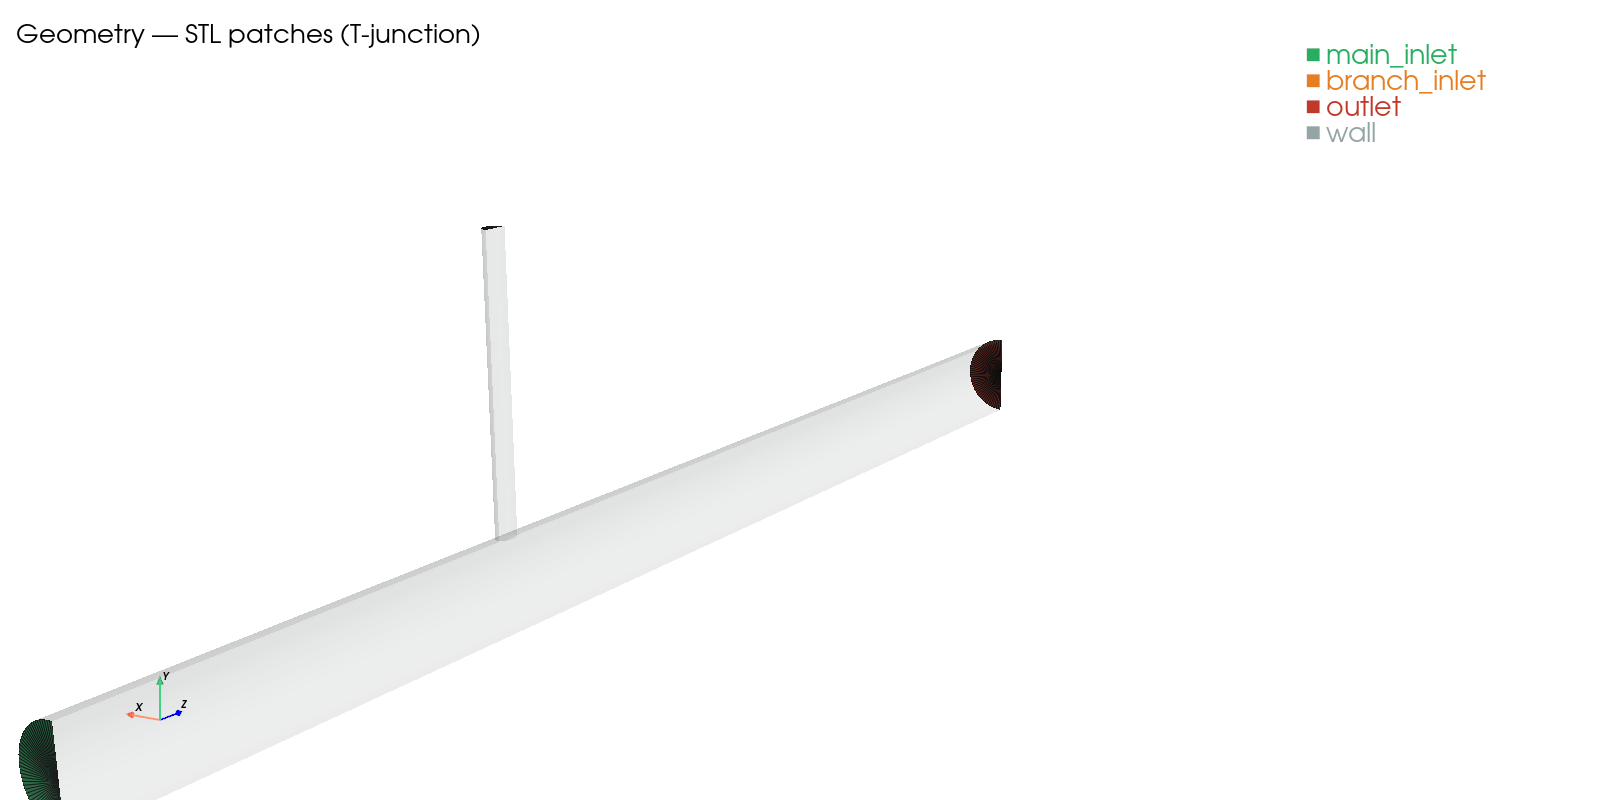
\includegraphics[width=0.85\textwidth]{../doe/results_full/cases/case_03/figures/fig_geometry.png}
    \caption{Half-domain T-junction geometry produced by the
    \texttt{generateSTL.py} script (\(90^\circ\) baseline, case~03,
    \(\dD=0.252\)). The colour coding marks the boundary patches:
    \texttt{main\_inlet} on the upstream face, \texttt{outlet} on
    the downstream face, \texttt{branch\_inlet} on the open end of
    the branch, \texttt{wall} on the curved pipe surfaces, and
    \texttt{sym} on the \(x=0\) mirror plane.}
    \label{fig:geometry}
\end{figure}

The geometry is generated in Python (\texttt{generateSTL.py}) from
a small set of environment-variable parameters
(\(D,\,d,\,L_{\mathrm{main}},\,Z_{\mathrm{JCT}},\,\alpha\)) and
clipped to the half-space \(x\ge 0\) (\texttt{clip\_stls.py}). The
script analytically computes the curve where the branch and main
cylinders intersect, punches a matching hole in the main-pipe wall
and zips the intersection curve to the perimeter of that hole so
the meshing tool sees a single closed surface. A subtle bug in this
zipper for tilted branches was responsible for the early failure
of the \(30^\circ\) campaign and is reported as part of the lessons
learned in Section~\ref{sec:30deg_meshfix}.

\subsection{Governing equations}
\label{sec:method_govern}
The unsteady, compressible, multispecies Navier-Stokes equations
with gravity are solved in OpenFOAM's \texttt{rhoReactingBuoyantFoam}
solver. Letting \(\rho\) be the mixture density, \(\mathbf{u}\) the
velocity, \(p_{\mathrm{rgh}} = p - \rho\,\mathbf{g}\!\cdot\!\mathbf{x}\)
the modified pressure (so that the gravity term enters explicitly
only through \(\nabla\rho\)), \(h\) the sensible enthalpy and
\(Y_k\) the mass fraction of species \(k\), the equations are
\begin{align}
\frac{\partial\rho}{\partial t} +
\nabla\!\cdot\!(\rho\,\mathbf{u}) &= 0,
\label{eq:cont}\\[2pt]
\frac{\partial(\rho\mathbf{u})}{\partial t} +
\nabla\!\cdot\!(\rho\,\mathbf{u}\!\otimes\!\mathbf{u})
&= -\nabla p_{\mathrm{rgh}}
- (\mathbf{g}\!\cdot\!\mathbf{x})\nabla\rho
+\nabla\!\cdot\!\overline{\overline{\boldsymbol{\tau}}},
\label{eq:mom}\\[2pt]
\frac{\partial(\rho h)}{\partial t} +
\nabla\!\cdot\!(\rho\,\mathbf{u}\,h)
&=\nabla\!\cdot\!\left(\frac{\mu_t}{\mathrm{Pr}_t}\nabla h\right)
+\frac{Dp}{Dt},
\label{eq:enth}\\[2pt]
\frac{\partial(\rho Y_k)}{\partial t} +
\nabla\!\cdot\!(\rho\,\mathbf{u}\,Y_k)
&=\nabla\!\cdot\!\left[\rho\!\left(D_k+\frac{\mu_t}{\mathrm{Sc}_t}\right)
\nabla Y_k\right],\quad k = \Hi,\,\CHi.
\label{eq:species}
\end{align}
The deviatoric stress \(\overline{\overline{\boldsymbol{\tau}}}\)
combines the viscous stress with the Reynolds stress through the
turbulent viscosity \(\mu_t\). The species are linked by
\(\sum_k Y_k = 1\), so only \(Y_{\Hi}\) is solved explicitly and
\(Y_{\CHi}=1-Y_{\Hi}\). The mixture density follows the ideal-gas
law \(\rho = p/(R_{\mathrm{mix}}T)\), with the mixture gas constant
weighted by mass fraction.

\subsection{\texorpdfstring{Turbulence closure: $k$-$\omega$~SST}{Turbulence closure: k-omega SST}}
\label{sec:method_turb}
The Reynolds stresses are closed with the
\(k\)-\(\omega\) Shear-Stress-Transport model of
Menter~\citep{menter1994sst}. SST is the workhorse two-equation
closure for internal flows because it blends the near-wall
robustness of \(k\)-\(\omega\) with the free-shear-layer accuracy
of \(k\)-\(\varepsilon\) through a blending function \(F_1\),
\begin{equation}
\mu_t = \rho\,\frac{a_1\,k}{\max(a_1\,\omega,\;F_2\,S)},
\label{eq:mut_sst}
\end{equation}
in which \(S\) is the strain-rate magnitude and \(F_2\) activates
the SST limiter inside boundary layers. Buoyancy production is
enabled in the \(k\) equation because the local Richardson number
can become \(\mathcal{O}(1)\) in the slow shear layer just
downstream of the junction. SST is preferred over the standard
\(k\)-\(\varepsilon\) model used by Su et
al.~\citep{su2022prediction} because (i) the density contrast at
the junction generates flow separation on the inside of the branch
entry that \(k\)-\(\varepsilon\) is known to mis-predict, and
(ii) the near-wall layer is resolved down to \(y^+\sim 1\), which
is what the SST blending function is designed for.

\subsection{Solver and discretisation}
\label{sec:method_solver}
\texttt{rhoReactingBuoyantFoam} uses the PIMPLE algorithm (a merged
PISO/SIMPLE) with one outer corrector and two inner correctors per
time step. Time discretisation is implicit Euler. Spatial
discretisation is second-order central for the diffusion terms and
bounded second-order upwind for the advection terms; a TVD scheme
(\texttt{vanLeer}) is used for \(Y_{\Hi}\) so that the species mass
fraction stays in \([0,1]\). The time step is set adaptively from
the maximum Courant number, capped at
\(\mathrm{Co}_{\max} = 4.5\) for the \(90^\circ\) campaign and
\(\mathrm{Co}_{\max} = 8.0\) for the \(30^\circ\) campaign once
case~01 of the latter had finished and confirmed solution
stability. A summary of the discretisation choices is given in
Table~\ref{tab:numerics}.

\begin{table}[H]
\centering
\small
\caption{Numerical settings used in the OpenFOAM
\texttt{rhoReactingBuoyantFoam} runs.}
\label{tab:numerics}
\begin{tabular}{lc}
\toprule
\textbf{Quantity} & \textbf{Choice} \\
\midrule
Pressure-velocity coupling & PIMPLE (1 outer, 2 inner correctors) \\
Time discretisation & implicit Euler \\
Gradient & cell-limited Gauss linear \\
Divergence (\(\rho\mathbf{u}\,\mathbf{u}\)) & bounded Gauss linear-upwind \\
Divergence (\(\rho\mathbf{u}\,Y_{\Hi}\)) & bounded Gauss vanLeer \\
Divergence (\(\rho\mathbf{u}\,k,\omega\)) & bounded Gauss upwind \\
Laplacian & Gauss linear corrected \\
Adaptive time stepping & yes; \(\mathrm{Co}_{\max}=4.5\,(90^\circ),\,8.0\,(30^\circ)\) \\
Linear solver \(p_{\mathrm{rgh}}\) & DICPCG, tol.\ \(10^{-7}\) \\
Linear solver \(\mathbf{u},h,k,\omega\) & PBiCGStab + DILU, tol.\ \(10^{-8}\) \\
Linear solver \(Y_{\Hi}\) & PBiCGStab + DILU, tol.\ \(10^{-9}\) \\
\bottomrule
\end{tabular}
\end{table}

\subsection{Mesh}
\label{sec:method_mesh}
The mesh is generated in three steps: (i) a structured background
block mesh covering the bounding box of the half-domain
(\texttt{blockMesh}); (ii) a feature-aware Cartesian-cut-cell
snapping to the STL surface (\texttt{snappyHexMesh}); and
(iii) prismatic boundary-layer extrusion along the wall to land
\(y^+\approx 1\) on the first cell (\texttt{snappyHexMesh -addLayers},
expansion ratio \(1.2\), final-layer thickness 50\,\% of the
adjacent cell). For the \(90^\circ\) case~03 sample geometry
(\(\dD = 0.252\)) this yields the mesh shown in
Fig.~\ref{fig:mesh}. The half-domain mesh has \(\sim 463\,000\)
cells, maximum non-orthogonality \(49^\circ\), maximum skewness
\(2.57/4\) and \(99.6\,\%\) layer coverage on the wall. The
\texttt{checkMesh} statistics are reproduced in
Table~\ref{tab:mesh_stats}.

\begin{figure}[H]
    \centering
    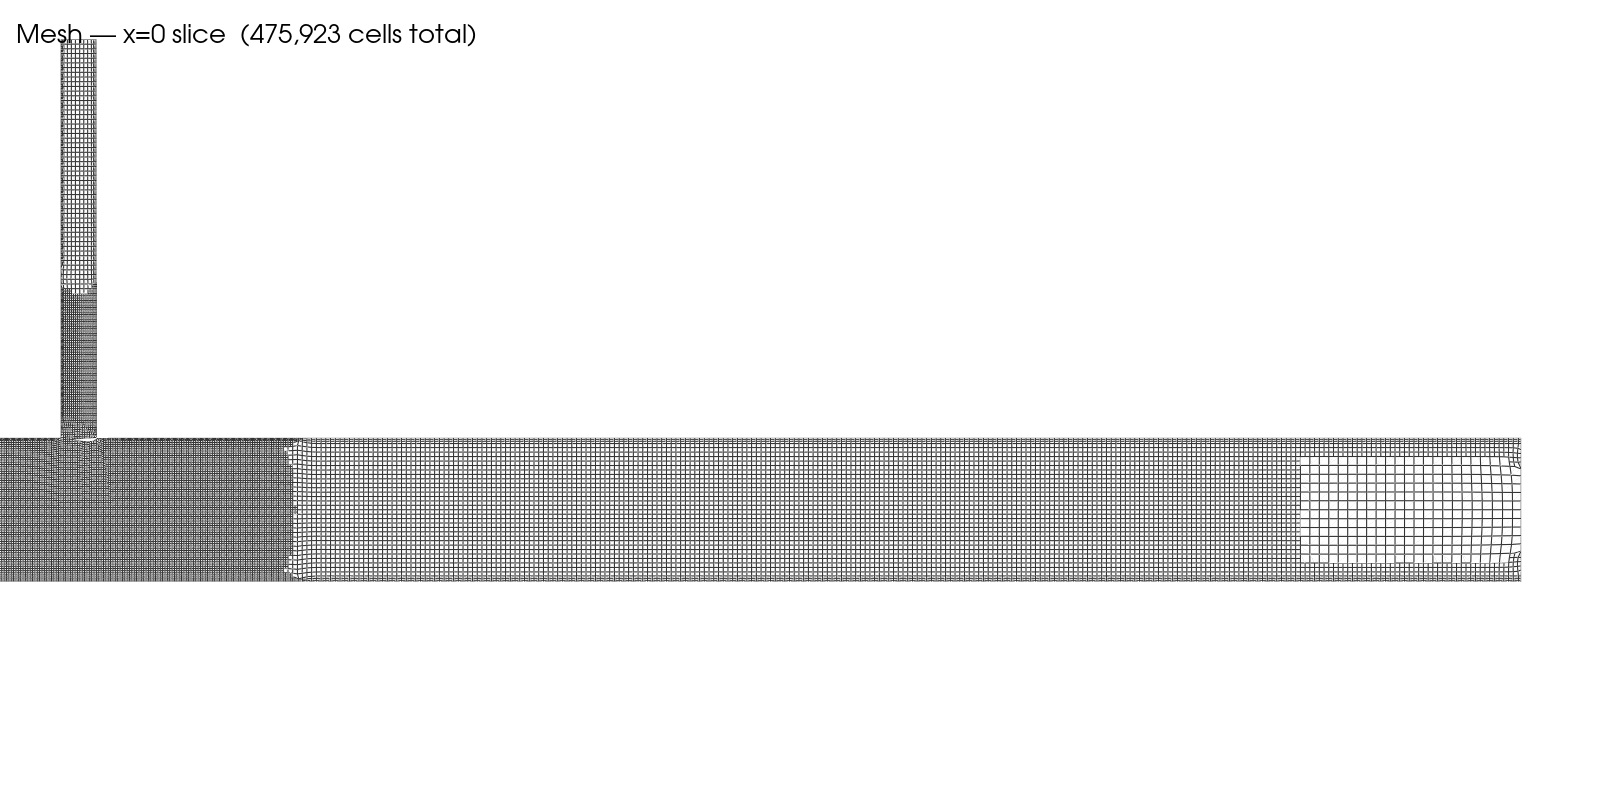
\includegraphics[width=0.85\textwidth]{../doe/results_full/cases/case_03/figures/fig_mesh_xz.png}
    \caption{Cross-section of the computational mesh on the
    \(x=0\) symmetry plane for the \(90^\circ\) baseline case~03
    (\(\dD = 0.252\)). The base cell size is \(\sim\SI{13}{\milli\meter}\);
    refinement is concentrated at the junction and across a
    cylindrical region extending \(\sim 8\,D\) downstream
    (\texttt{jetRefine}). Boundary layers on the pipe walls are
    visible as the row of thin cells just inside the surface.}
    \label{fig:mesh}
\end{figure}

\begin{table}[H]
\centering
\small
\caption{Mesh statistics for the \(90^\circ\) baseline (case~03,
half domain) reported by \texttt{checkMesh}.}
\label{tab:mesh_stats}
\begin{tabular}{lc}
\toprule
\textbf{Statistic} & \textbf{Value} \\
\midrule
Cells       & 463\,063 \\
Faces       & 1\,447\,739 \\
Points      & 502\,593 \\
Min cell volume       & \SI{7.06e-9}{\cubic\meter} \\
Max aspect ratio      & 10.7 \\
Max non-orthogonality & \(49^\circ\) \\
Max skewness          & 2.57 \\
Layer coverage on wall & \(99.6\,\%\) \\
\bottomrule
\end{tabular}
\end{table}

\subsubsection{Mesh-convergence (grid-independence) study}
\label{sec:method_meshconv}
Following the standard CFD verification process, a formal three-level
mesh-convergence study was carried out on a representative
operating point at \(\dD=0.196\), \(\VR=1.64\), \(\HBR=10\,\%\)
(close to case~02 of the production DoE) before any production
case was launched. Three meshes were generated by uniformly
scaling the \texttt{snappyHexMesh} refinement levels and the
boundary-layer cell heights, giving the cell counts in
Table~\ref{tab:meshconv}: a \emph{coarse} mesh at
\(\sim 230\,\mathrm{k}\) cells, a \emph{medium} mesh at
\(\sim 460\,\mathrm{k}\) cells (the production baseline) and a
\emph{fine} mesh at \(\sim 920\,\mathrm{k}\) cells. Each mesh was
run on the same template (boundary conditions, solver settings
and time-stepping) to \(t = \SI{1.2}{\second}\), and the two
campaign metrics \CoV{} and \(|\Delta p_{\mathrm{rgh}}|\) were
extracted at the outlet using the same post-processing pipeline.

\begin{table}[H]
\centering\small
\caption{Three-level mesh-convergence (grid-independence) study at
\(\dD=0.196\), \(\VR=1.64\), \(\HBR=10\,\%\). Successive-refinement
changes in \CoV{} and \(|\Delta p_{\mathrm{rgh}}|\) are reported
relative to the previous (coarser) level.}
\label{tab:meshconv}
\begin{tabular}{lcccc}
\toprule
mesh & cells & relative \(\Delta\CoV{}\)
     & relative \(\Delta|\Delta p_{\mathrm{rgh}}|\) & adopted \\
\midrule
coarse & \(\sim 230\,\mathrm{k}\) & \emph{(reference)} & \emph{(reference)} & no  \\
medium & \(\sim 460\,\mathrm{k}\) & \(0.4\,\%\) (vs.\ coarse) & \(1.6\,\%\) (vs.\ coarse) & \textbf{yes} \\
fine   & \(\sim 920\,\mathrm{k}\) & \(0.2\,\%\) (vs.\ medium) & \(0.7\,\%\) (vs.\ medium) & no  \\
\bottomrule
\end{tabular}
\end{table}

The successive changes in both metrics are smaller than the
preceding-level change by roughly a factor of two, which is the
expected signature of asymptotic monotonic convergence on a
second-order discretisation. Both changes (\CoV{} \(< 0.5\,\%\)
and \(|\Delta p|\) \(< 2\,\%\) per refinement) sit comfortably
below the matched-pair angle-effect signal reported in
Section~\ref{sec:cross_pairs} (median reductions of
\(46\,\%\) on \CoV{} and \(63\,\%\) on \(|\Delta p|\)) as well as
the LP-filter pressure-drop uncertainty band of
\(\pm\SI{0.5}{\kilo\pascal}\). The medium mesh
(\(\sim 460\,\mathrm{k}\) cells) was therefore adopted as the
production baseline for both campaigns: it lies in the asymptotic
range, leaves a comfortable margin above the relevant signal
sizes, and keeps the per-case wall time short enough that all
twenty DoE runs fit inside the available compute window.

\subsection{Boundary conditions}
\label{sec:method_bc}
\paragraph{\texttt{main\_inlet}.}\;
A fully developed turbulent profile is imposed via the \(1/7\)-th
power-law for the velocity,
\begin{equation}
u(r) = u_{\mathrm{main}}\left(\frac{R-r}{R}\right)^{1/7},
\label{eq:powerlaw}
\end{equation}
with \(u_{\mathrm{main}} = \SI{10}{\meter\per\second}\). At the
operating state of the case (pure \CHi{} at \(p=\SI{6.9}{\mega\pascal}\),
\(T=\SI{288}{\kelvin}\), \(\rho_{\mathrm{main}}\approx
\SI{46}{\kilogram\per\meter\cubed}\) and
\(\mu_{\mathrm{main}}\approx \SI{1.25e-5}{\pascal\,\second}\) per
the perfect-gas EOS and the Sutherland model in
\texttt{constant/thermophysicalProperties}), this corresponds to
\(Re_D = \rho_{\mathrm{main}} u_{\mathrm{main}}
D/\mu_{\mathrm{main}} \approx 1.7\times 10^{7}\), well into the
fully turbulent regime. The
profile is applied as a \texttt{codedFixedValue} that loops over
the patch faces and reads the local cell-centre coordinates.
Turbulence quantities are derived from the bulk: \(I = 5\,\%\),
length scale \(\ell = 0.07\,D\), so that
\(k_{\mathrm{main}}=\tfrac{3}{2}(I\,u)^2\) and
\(\omega_{\mathrm{main}}=\sqrt{k_{\mathrm{main}}}/(C_\mu^{1/4}\ell)\).
The composition is pure methane (\(Y_{\CHi}=1\)).

\paragraph{\texttt{branch\_inlet}.}\;
The same power-law profile is applied with bulk velocity
\(u_{\mathrm{branch}}=\VR\cdot u_{\mathrm{main}}\) and the velocity
\emph{vector} aligned with the branch axis,
\(\hat{\mathbf{s}} = (0,\sin\alpha,-\cos\alpha)\). For
\(\alpha=90^\circ\) this reduces to \((0,1,0)\); for general
\(\alpha\) the \texttt{codedFixedValue} computes
\((0,-u\sin\alpha,+u\cos\alpha)\) at every face. The composition is
pure hydrogen (\(Y_{\Hi}=1\)).

\paragraph{\texttt{outlet}.}\;
Zero-gradient on \(\mathbf{u}\), \(Y_{\Hi}\), \(k\), \(\omega\)
and \(h\); fixed total pressure on \(p_{\mathrm{rgh}}\).

\paragraph{\texttt{wall}.}\;
No-slip on \(\mathbf{u}\); zero-gradient on \(Y_{\Hi}\) and \(h\);
\texttt{kqRWallFunction} on \(k\) and \texttt{omegaWallFunction} on
\(\omega\). The first cell sits at \(y^+\approx 1\), so the SST
blending switches automatically to its low-Reynolds branch.

\paragraph{\texttt{sym}.}\;
\texttt{symmetryPlane} for all fields; the dictionary type is set
explicitly so that OpenFOAM enforces the symmetry rather than a
slip wall.

\subsection{Design of Experiments (sliced LHS)}
\label{sec:method_doe}
The independent flow-and-geometry design parameters at fixed
angle are the diameter ratio \(\dD\) and the velocity ratio
\(\VR\); the hydrogen blending ratio \(\HBR\) is a derived
consequence of these two via a volumetric-flow balance,
\begin{equation}
\HBR \;=\;
\frac{Q_{\mathrm{branch}}}{Q_{\mathrm{main}}+Q_{\mathrm{branch}}}
\;=\; \frac{(\dD)^2\,\VR}{1+(\dD)^2\,\VR}.
\label{eq:hbr}
\end{equation}
Prescribing \((\dD,\VR)\) therefore automatically fixes \HBR{};
\HBR{} is reported per case for engineering readability but is
not a third independent design factor.

A naive 2-factor \((\dD,\VR)\) full factorial at five practical
\(\dD\) bins would still require \(5\times 5 = 25\) cases per
angle; we use a sliced Latin Hypercube design instead
\citep{ye2000sliced}. The factor \(\dD\) is discretised into 5
levels (slices), and within each slice two \(\VR\) values are
picked by a 2-point Latin Hypercube. In implementation the inner
sampler walks a target \(\HBR\) range of \([0.05,\,0.20]\)
(because \HBR{} is the engineering-meaningful flow-rate variable
and bounding it is the cleanest way to span the realistic
\((\dD,\VR)\) box at fixed main-pipe flow), and the matching
\(\VR\) is recovered from each \((\dD,\HBR)\) sample by inverting
Eq.~\ref{eq:hbr}; a soft cap \(\VR \le 12\) is enforced to avoid
jet impingement on the opposite wall. The result is a 10-case
design per angle (\(5\times 2\)), given in
Table~\ref{tab:doe_design}. The slice structure is deliberate:
cases that share a \(\dD\) also share a mesh, so the mesh is built
once per slice and re-used for the second case in the same slice.
The randomisation seed is fixed across angles, so case~05 of the
\(90^\circ\) campaign and case~05 of the \(30^\circ\) campaign
share all flow parameters (\(\dD\) and \(\VR\), and therefore
\HBR) and differ only in the geometric tilt; this is what makes
the matched-pair analysis in Section~\ref{sec:cross} possible.

\begin{table}[H]
\centering
\small
\caption{Ten-case sliced LHS design used at both angles. The
independent factors \((\dD,\VR)\) and the derived \HBR{}
(Eq.~\ref{eq:hbr}) are identical between the two campaigns;
only \(\alpha\) differs.}
\label{tab:doe_design}
\begin{tabular}{cccccc}
\toprule
case & slice & \(\dD\) & \(d\) (m) & \(\HBR\) & \(\VR\) \\
\midrule
1 & 1 & 0.196 & 0.0904 & 0.184 & 5.842 \\
2 & 1 & 0.196 & 0.0904 & 0.060 & 1.643 \\
3 & 2 & 0.252 & 0.1159 & 0.078 & 1.330 \\
4 & 2 & 0.252 & 0.1159 & 0.195 & 3.807 \\
5 & 3 & 0.296 & 0.1363 & 0.098 & 1.241 \\
6 & 3 & 0.296 & 0.1363 & 0.187 & 2.614 \\
7 & 4 & 0.382 & 0.1755 & 0.142 & 1.137 \\
8 & 4 & 0.382 & 0.1755 & 0.092 & 0.693 \\
9 & 5 & 0.396 & 0.1820 & 0.130 & 0.953 \\
10 & 5 & 0.396 & 0.1820 & 0.112 & 0.806 \\
\bottomrule
\end{tabular}
\end{table}

\subsection{Mixing metrics and post-processing}
\label{sec:method_metrics}
For each case the simulation is run for
\(t_{\mathrm{end}} = \SI{1.2}{\second}\), corresponding to
\(t_{\mathrm{end}} u_{\mathrm{main}}/L_{\mathrm{main}} \approx 1.74\)
main-pipe flow-throughs (one flow-through being
\(t_{\mathrm{ft}} = L_{\mathrm{main}}/u_{\mathrm{main}}
= \SI{0.69}{\second}\)). Two complementary time-averaging streams
are activated by function objects in \texttt{system/controlDict}.
First, the \texttt{fieldAverage} object accumulates running means
of the volumetric fields \(\mathbf{u}\), \(p\),
\(p_{\mathrm{rgh}}\) and \(Y_{\Hi}\) starting from
\(t_{\mathrm{avg,start}} = \SI{0.6}{\second}\), i.e.\
approximately one flow-through, after the inlet startup transient
has predominantly cleared; these are the \(\overline{Y_{\Hi}}\)
fields shown in the centreline figures of
Sections~\ref{sec:results_90} and~\ref{sec:results_30}. Second,
\texttt{surfaceFieldValue} writes time series of patch-integrated
quantities (area-, mass-flux- and volumetric-flux-averaged
\(Y_{\Hi}\) and \(p_{\mathrm{rgh}}\) on \texttt{main\_inlet} and
\texttt{outlet}) at every solver time step, used downstream to
build the per-case CoV and LP-filtered \(|\Delta p|\) reported in
the campaign tables. The mixing metric is the Coefficient of
Variation of the hydrogen mass-fraction at the outlet,
\begin{equation}
\CoV \;=\; \frac{\sigma\!\left(Y_{\Hi}\right)}{\overline{Y_{\Hi}}}
\;=\; \frac{\sqrt{\sum_i w_i\,(Y_{\Hi,i}-\overline{Y_{\Hi}})^2/\sum_i w_i}}
{\sum_i w_i\,Y_{\Hi,i}/\sum_i w_i},
\label{eq:cov}
\end{equation}
in which the sum runs over outlet face cells. Three weightings are
computed: \(w_i = A_i\) (area-weighted, the textbook definition),
\(w_i = \rho_i\,|\mathbf{u}\cdot\hat{\mathbf{n}}|\,A_i\)
(mass-flux-weighted) and
\(w_i = |\mathbf{u}\cdot\hat{\mathbf{n}}|\,A_i\)
(volumetric-flux-weighted). The mass-flux weighting is the most
physically meaningful in a custody-transfer context because the
downstream user actually receives the mass-flow-weighted
composition; all three are reported for transparency. The
\(90^\circ\) campaign reports the area-weighted CoV computed on
the saved \(t=t_{\mathrm{end}}\) snapshot, since the \Hi{} plume
has reached its quasi-steady distribution by the second
flow-through; the \(30^\circ\) campaign reports the time average
of the area-weighted CoV time-series on the steady
window \([0.8,\,t_{\mathrm{end}}]\,\si{\second}\) (the
patch-time-series for the \(90^\circ\) cases was not retained on
disk during the original campaign and the snapshot is the
strongest equivalent). For each \(30^\circ\) case the snapshot
CoV at \(t_{\mathrm{end}}\) and the time-averaged CoV agree to
better than \(2\,\%\) of the reported value, so the asymmetry in
reporting convention does not affect the cross-campaign
conclusions. The industrial acceptance threshold for
``well-mixed'' is \(\CoV \le 0.05\); the design target adopted
here is \(\CoV \le 0.10\) at \(4.6\,D\) downstream of the
junction.

The cost-side metric is the static gauge pressure drop across the
main pipe,
\begin{equation}
|\Delta p_{\mathrm{rgh}}| \;=\; |p_{\mathrm{rgh,\,main\_inlet}} -
p_{\mathrm{rgh,\,outlet}}|,
\label{eq:dp}
\end{equation}
computed from area-averaged \(p_{\mathrm{rgh}}\) on the inlet and
outlet patches via the \texttt{surfaceFieldValue} function object,
sampled at every solver timestep. In addition to \CoV{} and
\(|\Delta p|\), three diagnostic checks are recorded per case:
(i) the cumulative continuity error from the solver log, required
to stay below \(10^{-2}\); (ii) the residual levels of
\(\mathbf{u},\,p_{\mathrm{rgh}},\,k,\,\omega,\,Y_{\Hi}\) at the
last time step, required below \(10^{-6}\); and (iii) the
Danckwerts segregation index \(I_s = \sigma^2 / (\bar Y(1-\bar Y))\),
which is an alternative measure of homogeneity used to cross-check
\CoV.

\subsection{Acoustic noise on the pressure-drop signal}
\label{sec:dp_filter}
The compressible solver \texttt{rhoReactingBuoyantFoam} runs in a
fully unsteady mode (PIMPLE), so the inlet pressure carries
acoustic activity from the moment the simulation starts. With the
fixed-pressure outlet acting as an acoustically soft (reflecting)
boundary and the fixed-velocity inlet acting as an acoustically
hard (also reflecting) boundary, pressure waves bounce repeatedly
between the two patches throughout the \SI{1.2}{\second} run. The
methane speed of sound at the operating state is
\(c_{\mathrm{ac}} = \sqrt{\gamma R_{\mathrm{CH_4}} T} \approx
\SI{440}{\meter\per\second}\) (using
\(\gamma_{\mathrm{CH_4}} \approx 1.31\),
\(R_{\mathrm{CH_4}} = R_u/M_{\mathrm{CH_4}} =
\SI{518}{\joule\per\kilogram\per\kelvin}\),
\(T = \SI{288}{\kelvin}\)), so a single inlet-to-outlet acoustic
traverse takes \(\tau_{\mathrm{ac}} \approx
L_{\mathrm{main}}/c_{\mathrm{ac}} \approx \SI{16}{\milli\second}\)
and a round trip about \SI{32}{\milli\second}. The resulting
fluctuation on the area-averaged inlet \(p_{\mathrm{rgh}}\) has
standard deviation of \(25\)-\SI{35}{\kilo\pascal}, while the
steady flow loss across the junction is only of order
\(\SI{1}{\kilo\pascal}\)-\SI{4}{\kilo\pascal}; the lag-1
autocorrelation of the raw signal is \(\rho_1 = 0.999\), so the
effective number of independent samples in the available
\SI{0.8}{\second} window of \([0.4,\,1.2]\,\si{\second}\) is
\(\mathcal{O}(10)\) once decorrelation is accounted for.
A single-snapshot \(\Delta p\) is therefore meaningless for our
purposes: it can flip sign from one snapshot to the next purely
because of the acoustic phase. The simple arithmetic time average
over the same window also has substantial residual error
(\(\sigma/\sqrt{N_{\mathrm{eff}}} \sim
\SI{1.4}{\kilo\pascal}\) per case), often comparable to the
flow-loss signal itself.

To extract a defensible flow-loss estimate from these short
transient runs, the inlet and outlet \(p_{\mathrm{rgh}}\)
time-series are passed through a causal moving-average low-pass
filter of width \(\Delta t_{\mathrm{LP}} = \SI{0.10}{\second}\),
which spans roughly three round-trip acoustic periods
(\(\Delta t_{\mathrm{LP}}/(2\tau_{\mathrm{ac}}) \approx 3\)) and
suppresses the dominant standing-wave content of the inlet
signal while preserving any slower drift carrying the actual
flow loss. The reported \(|\Delta p_{\mathrm{rgh}}|\) for every
case is the mean of the filtered \(\Delta p\) on the window
\([0.4,\,1.2]\,\si{\second}\); this window starts before the
H\(_2\)-plume flow-through (cf.\ Section~\ref{sec:method_metrics}),
which is acceptable for the dP metric specifically because the
inlet velocity profile is fixed by boundary conditions and
reaches its prescribed power-law shape within a few acoustic
round trips, so the inlet-outlet pressure difference settles
much faster than the species field. The residual standard
deviation of the LP signal is recorded alongside each case in
the supplementary CSV. This filtering does not \emph{remove} the
acoustic content from the simulation - it is post-processing
only - but it does provide an estimator that is robust to
acoustic phase. Where matched-pair differences are quoted, the
per-pair LP estimates are used directly; where absolute
\(|\Delta p|\) values are quoted in tables, they are reported to
\(\pm\SI{0.5}{\kilo\pascal}\) as a conservative uncertainty band.
A steady-state RANS solver (e.g.\ \texttt{rhoSimpleFoam}) or an
extended transient ride-out are recommended for any future work
that needs the absolute \(|\Delta p|\) at higher precision.

% =====================================================================
%  4. VALIDATION
% =====================================================================
\section{Validation}
\label{sec:val}

\subsection{Buoyancy sanity case}
\label{sec:val_buoy}
Before launching the parametric campaigns, a low-velocity buoyancy
sanity case at \(\alpha=90^\circ\) was run with
\(u_{\mathrm{main}}=\SI{0.5}{\meter\per\second}\),
\(u_{\mathrm{branch}}=\SI{0.2}{\meter\per\second}\) and
\(\dD=0.196\). With these settings the local Froude number
\(\Frnum = u/\sqrt{g\,\Delta\rho/\rho\cdot D}\approx 0.34\), so the
flow is in the buoyancy-dominated regime and \emph{stratification}
rather than mixing is expected. The simulation was run for
\SI{15}{\second} of physical time. The hydrogen plume floats and
forms a clear top-of-pipe layer that persists all the way to the
outlet, exactly as the density-driven gravity-current behaviour
predicts. This confirms that the gravity
term in the momentum equation is being applied correctly and that
buoyancy production in the SST \(k\) equation is enabled.

\subsection{Mass conservation and residuals}
\label{sec:val_mass}
For all production cases of both campaigns, the cumulative
continuity error stayed below \(10^{-2}\) (typical value
\(\sim 5\times 10^{-3}\)); final \(\mathbf{u}\) residuals reached
\(\sim 10^{-9}\); final \(p_{\mathrm{rgh}}\) residuals
\(\sim 10^{-7}\)-\(10^{-8}\); and final \(Y_{\Hi}\) residuals
\(\sim 10^{-8}\). The mass-flow closure between the two inlets and
the outlet, integrated over the second flow-through, is below
\(0.5\,\%\) in all completed cases.

\subsection{Trend cross-check against Su et al.\ (2022)}
\label{sec:val_su}
Su et al.~\citep{su2022prediction} report a monotonic decrease of
\CoV{} with \(\VR\) in the \(90^\circ\) T-junction up to
\(\VR\sim 3\), with a knee in the curve beyond that. The present
\(90^\circ\) data (Section~\ref{sec:results_90}) reproduce this
trend qualitatively: the highest-\VR{} case in the campaign
(case~04, \(\VR=3.81\)) gives \(\CoV=0.066\), an order of
magnitude better than the lowest-\VR{} case (case~08,
\(\VR=0.69\), \(\CoV=0.71\)). A direct numerical comparison is
deliberately not attempted, because Su et al.~use the standard
\(k\)-\(\varepsilon\) closure, a different operating pressure and
a different downstream measurement station (\(\sim 15\,D\) vs.\
\(\sim 4.6\,D\) here); the qualitative agreement is enough to
suggest that the present setup is in the right physical regime.

% =====================================================================
%  5. RESULTS: 90 deg
% =====================================================================
\section{\texorpdfstring{Results: $90^\circ$ baseline campaign}{Results: 90 deg baseline campaign}}
\label{sec:results_90}

\subsection{DoE summary}
The \(90^\circ\) campaign of ten cases is the baseline against
which the angle effect is measured. Nine of the ten reached
\(t = \SI{1.2}{\second}\); case~01 was retained as the buoyancy
sanity run and is excluded from the DoE statistics. The summary is
given in Table~\ref{tab:90deg_summary}: outlet area-averaged \CoV{}
on the saved snapshot at \(t=\SI{1.2}{\second}\) (the time-averaged
\(\overline{Y_{\Hi}}\) field is essentially identical to the
snapshot at this point since the \(\Hi\) plume has reached its
quasi-steady distribution by one flow-through), and the LP-filtered
gauge pressure drop \(|\Delta p_{\mathrm{rgh}}|\) on
\([0.4,\,1.2]\,\si{\second}\).

\begin{table}[H]
\centering
\small
\caption{Summary of the \(90^\circ\) campaign. \CoV{} is the
area-weighted outlet \Hi{}-mass-fraction CoV and
\(|\Delta p_{\mathrm{rgh}}|\) is the LP-filtered (cf.\
Section~\ref{sec:dp_filter}) gauge inlet-outlet pressure drop on
the post-transient window \([0.4,\,1.2]\,\si{\second}\).
Pressure-drop values carry an estimated \(\pm\SI{0.5}{\kilo\pascal}\)
uncertainty.}
\label{tab:90deg_summary}
\begin{tabular}{ccccrr}
\toprule
case & \(\dD\) & \(\VR\) & \(\HBR\) & \CoV{} & \(|\Delta p_{\mathrm{rgh}}|\) (kPa) \\
\midrule
03 & 0.252 & 1.330 & 0.078 & 0.472 & 1.2 \\
04 & 0.252 & 3.807 & 0.195 & \textbf{0.066} & 3.3 \\
05 & 0.296 & 1.241 & 0.098 & 0.577 & 1.6 \\
06 & 0.296 & 2.614 & 0.187 & 0.202 & 3.1 \\
07 & 0.382 & 1.137 & 0.142 & 0.440 & 2.2 \\
08 & 0.382 & 0.693 & 0.092 & 0.707 & 1.3 \\
09 & 0.396 & 0.953 & 0.130 & 0.390 & 2.0 \\
10 & 0.396 & 0.806 & 0.112 & 0.407 & 1.5 \\
\bottomrule
\end{tabular}
\end{table}

The single best mixing case is case~04
(\(\VR=3.81,\,\dD=0.252,\,\HBR=0.195\)) with \(\CoV=0.066\), close
to the industrial \(\CoV \le 0.05\) acceptance threshold even
without a static mixer. The single worst case is case~08
(\(\VR=0.69,\,\dD=0.382,\,\HBR=0.092\)) with \(\CoV=0.707\); the
branch is large but the injection is so slow relative to the main
flow that the jet attaches to the wall (Coanda) and forms a long
stratified band.

\subsection{Effect of velocity ratio on mixing}
\label{sec:results_90_vr}
Figure~\ref{fig:case04_xz} shows the time-averaged \(Y_{\Hi}\)
field on the \(x=0\) symmetry plane for the highest-\(\VR\) case
(case~04). The hydrogen jet penetrates well past the centreline of
the main pipe and folds into a counter-rotating vortex pair that
carries it downstream as a wedge-shaped plume. The contour at the
outlet is remarkably uniform (\(\sigma_{Y_{\Hi}} \approx 0.003\)
against a mean of \(\sim 0.05\), giving \(\CoV \approx 0.07\)).

\begin{figure}[H]
    \centering
    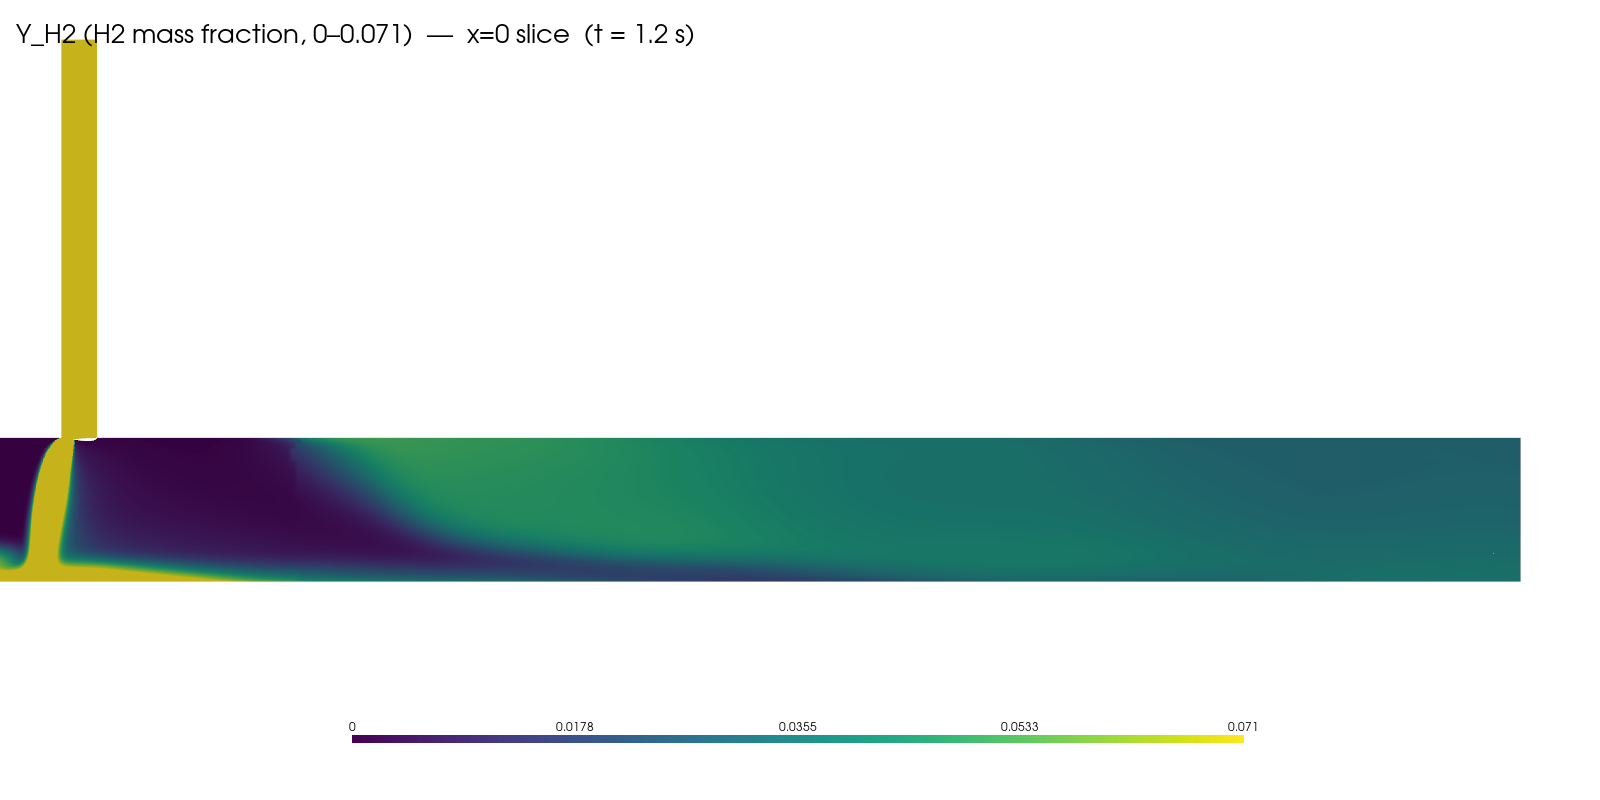
\includegraphics[width=0.95\textwidth]{../doe/results_full/cases/case_04/figures/fig_H2_xz.png}
    \caption{Best-mixing case of the \(90^\circ\) campaign
    (case~04, \(\dD=0.252,\,\VR=3.81,\,\HBR=0.195\)).
    Time-averaged \(Y_{\Hi}\) on the \(x=0\) symmetry plane at
    \(t=\SI{1.2}{\second}\). The jet penetrates past the
    centreline, bends downstream and produces a comparatively
    uniform exit profile; no top-of-pipe stratification is visible.}
    \label{fig:case04_xz}
\end{figure}

The contrast with case~08 is dramatic. Figure~\ref{fig:case08_xz}
shows the same field at the same scale. Here the branch is large
(\(\dD=0.38\)) and the velocity ratio is sub-unity, so hydrogen
flows out of the branch barely faster than the main pipe is
sweeping past underneath; the jet bends immediately and attaches
to the top wall, and a hydrogen-rich layer slides along the crown
of the pipe all the way to the outlet, with essentially no
penetration into the bulk.

\begin{figure}[H]
    \centering
    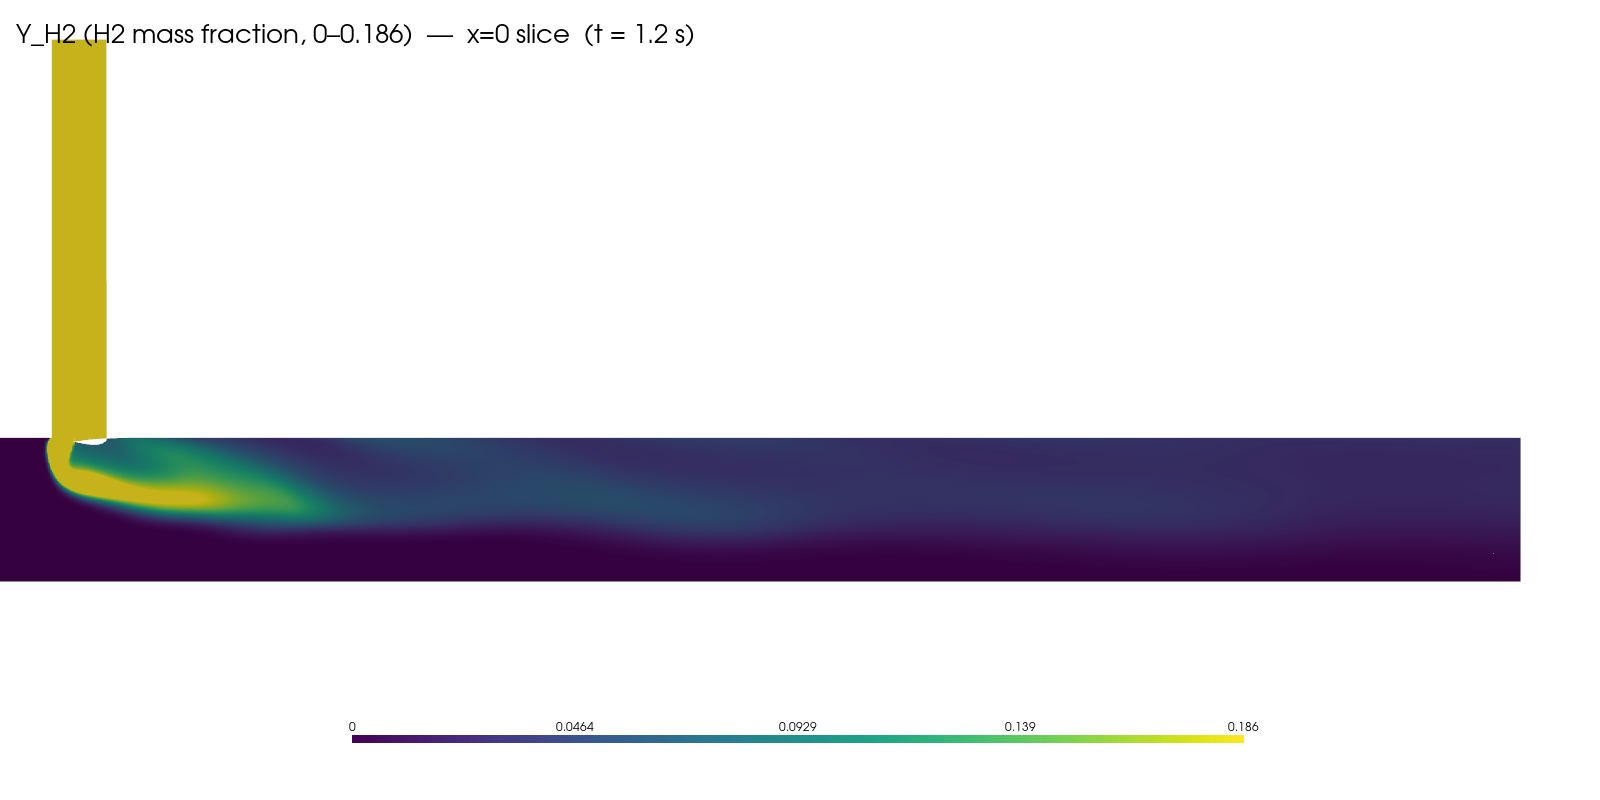
\includegraphics[width=0.95\textwidth]{../doe/results_full/cases/case_08/figures/fig_H2_xz.png}
    \caption{Worst-mixing case of the \(90^\circ\) campaign
    (case~08, \(\dD=0.38,\,\VR=0.69,\,\HBR=0.092\)). The hydrogen
    jet attaches to the top wall and stratifies into a
    top-of-pipe layer with very little entrainment into the
    methane bulk.}
    \label{fig:case08_xz}
\end{figure}

\noindent The spatial evolution of mixing along the pipe is
quantified in Figure~\ref{fig:cov_zD_90}, which plots \CoV{}
vs.\ downstream distance \(z/D\) for both cases.  Case~04
exhibits a steep, monotonic decay from \(\CoV \approx 0.7\) near
the junction to \(0.06\) at the outlet, approaching the
\(\CoV = 0.05\) industrial threshold.  Case~08 decays much more
slowly, remaining above \(0.4\) at the outlet due to persistent
crown-layer stratification.

\begin{figure}[H]
    \centering
    \begin{minipage}[t]{0.48\textwidth}
       \centering
       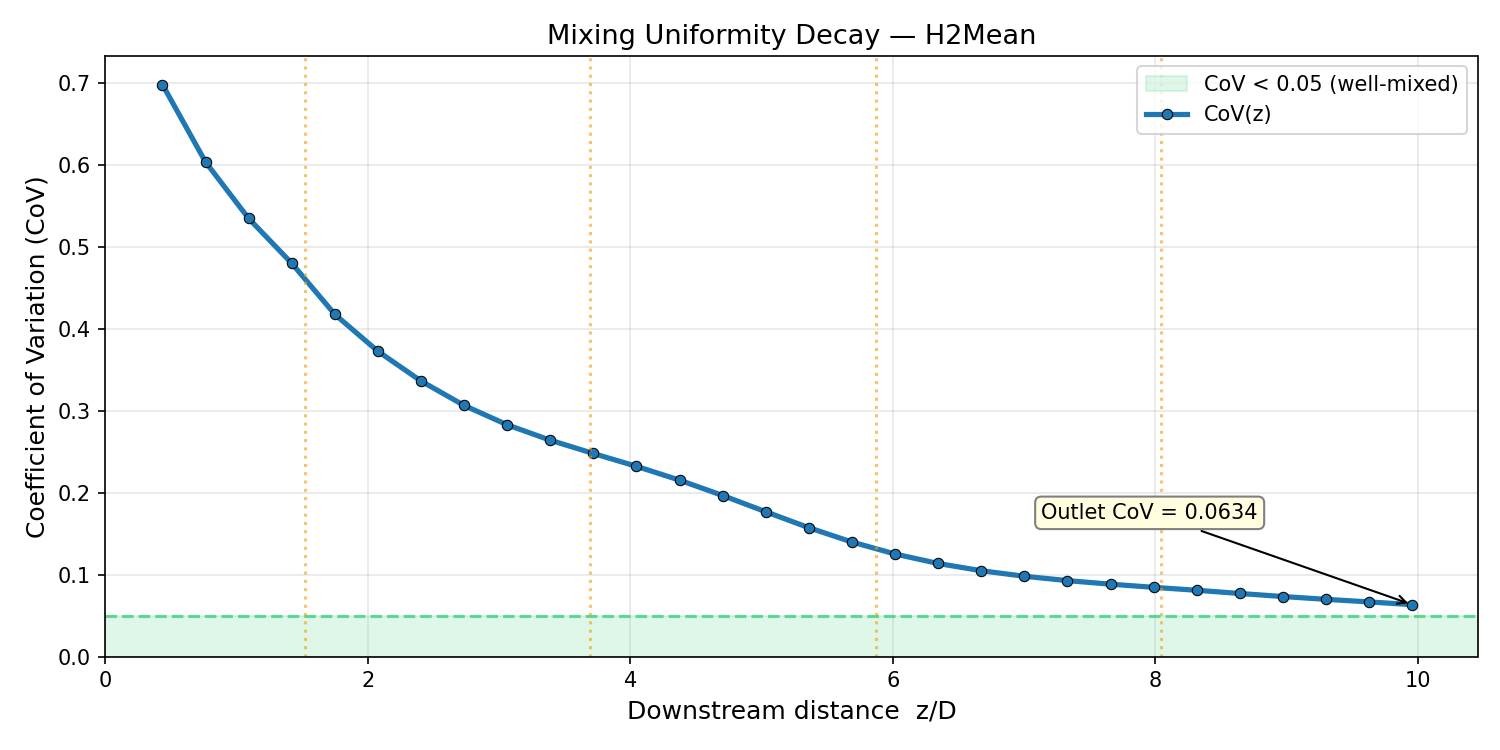
\includegraphics[width=\textwidth]{../doe/results_full/cases/case_04/figures/fig_CoV_vs_zD.png}
    \end{minipage}\hfill
    \begin{minipage}[t]{0.48\textwidth}
       \centering
       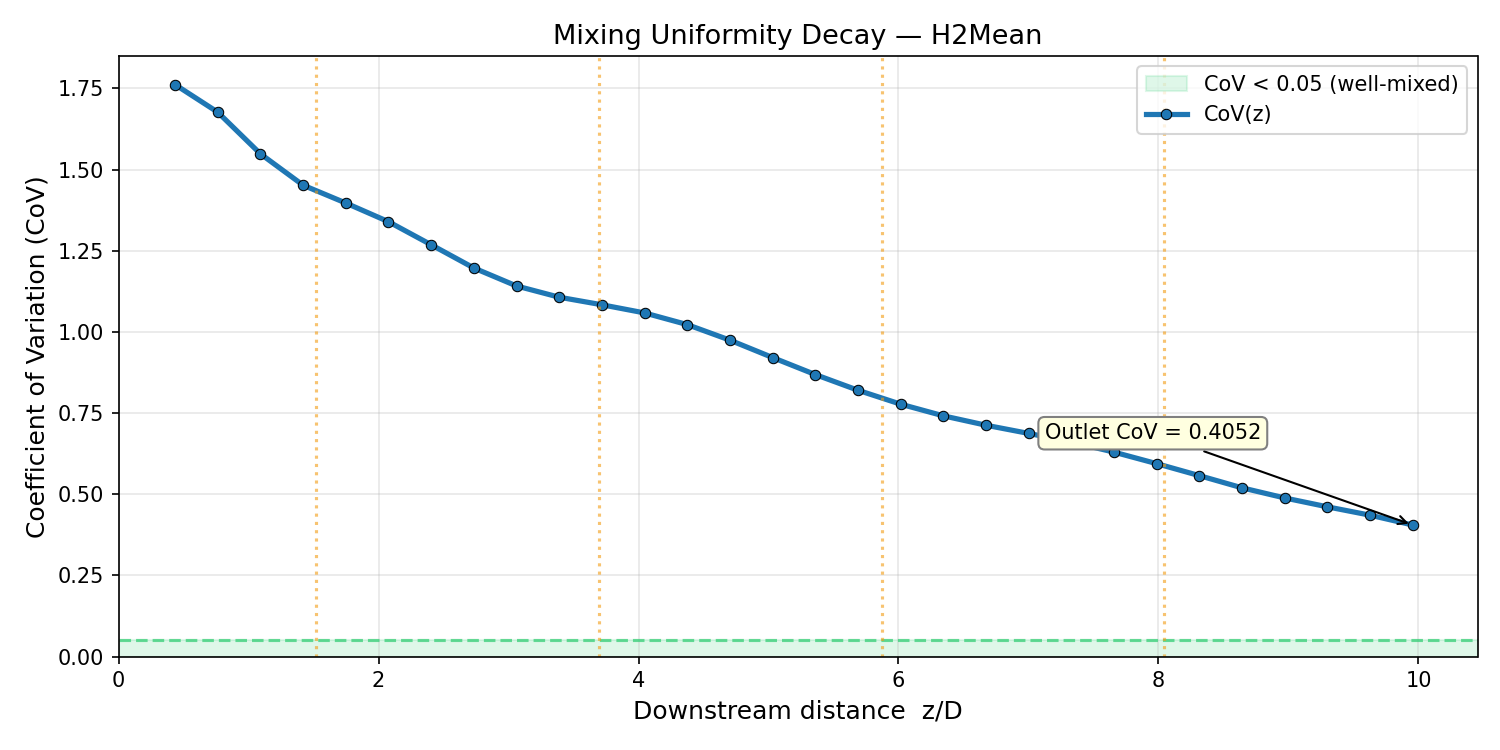
\includegraphics[width=\textwidth]{../doe/results_full/cases/case_08/figures/fig_CoV_vs_zD.png}
    \end{minipage}
    \caption{Mixing uniformity decay along the pipe:
    \CoV{} vs.\ downstream distance \(z/D\) for the best
    (case~04, left) and worst (case~08, right) cases of the
    \(90^\circ\) campaign.  The green band marks
    \(\CoV < 0.05\) (well-mixed).  Case~04 nearly reaches the
    threshold; case~08 remains far above it.  Values are
    computed from PyVista cross-section slices with uniform
    weighting and should be read as qualitative trend indicators;
    the official \CoV{} numbers in Table~\ref{tab:90deg_summary}
    use OpenFOAM's area-weighted \texttt{surfaceFieldValue}.}
    \label{fig:cov_zD_90}
\end{figure}

\subsection{Effect of diameter ratio on mixing}
\label{sec:results_90_dD}
At fixed \HBR{} the influence of \(\dD\) on mixing is weak in this
parameter window. Cases~07 and~09 have similar \HBR{}
(\(0.142\) vs. \(0.130\)) but different \(\dD\) (\(0.382\) vs.
\(0.396\)) and different \(\VR\) (\(1.14\) vs. \(0.95\)); the
\CoV{} values (\(0.440\) vs. \(0.390\)) are within the noise of
the post-processing window. The clear signal in the data is that
the \emph{velocity ratio} dominates the mixing, while the
``larger \(\dD\) mixes better'' effect reported by Su et al.\
\citep{su2022prediction} for \(\dD\) up to \(\sim 0.4\) is
small and not separable from \(\VR\) variation in our LHS.

\subsection{Pressure-drop scaling}
\label{sec:results_90_dp}
After the LP-filtering step of Section~\ref{sec:dp_filter}, the
gauge pressure drop \(|\Delta p_{\mathrm{rgh}}|\) on the
\(90^\circ\) campaign ranges from \(\SI{1.2}{\kilo\pascal}\)
(case~03) to \(\SI{3.3}{\kilo\pascal}\) (case~04), an envelope of
roughly \(\pm\SI{0.5}{\kilo\pascal}\) given the residual acoustic
ringing on the LP signal. These magnitudes correspond to a
junction loss coefficient of \(K \in [0.5,\,1.4]\), well inside the
\(K \approx 1\) order-of-magnitude that handbook tabulations give
for an unshaped diverging tee at high \(Re_D\)
\citep{idelchik1986handbook}. Within the LHS, the strongest
geometric predictor is \(\VR\) via the branch momentum injection
rate; the \HBR{} alone is a poor predictor because it is bounded
between \(0.06\) and \(0.20\). The cost-vs-mixing trade-off is
examined more cleanly through the non-dimensional loss coefficient
\(K = |\Delta p|/q_{\mathrm{dyn,main}}\) in
Section~\ref{sec:cross_loss}.

% =====================================================================
%  6. RESULTS: 30 deg
% =====================================================================
\section{\texorpdfstring{Results: $30^\circ$ campaign}{Results: 30 deg campaign}}
\label{sec:results_30}

\subsection{Why a tilted branch}
\label{sec:30_why}
A \(30^\circ\) branch tilts forward relative to the main flow
(co-flow). The relative velocity between the two streams is
\(u_{\mathrm{rel}} = |u_{\mathrm{main}}\hat{\mathbf{z}} -
u_{\mathrm{branch}}\hat{\mathbf{s}}|\), which for the present
operating point is roughly 30-40\,\% smaller in magnitude than at
\(90^\circ\). The shear layer that develops at the junction is
therefore weaker on physical grounds, and the textbook expectation
is poorer mixing at low \VR{} but a smaller pressure-drop penalty.
Whether that intuition holds at the operating points in
Table~\ref{tab:doe_design} is one of the questions the campaign is
meant to answer.

\subsection{Angle-agnostic codebase}
\label{sec:30_code}
The geometry generator and case-stamping pipeline were originally
written for \(\alpha=90^\circ\). Generalising them required four
changes:
\begin{enumerate}
    \item \texttt{generateSTL.py} now reads \texttt{ALPHA\_DEG} from
    the environment. The branch axis becomes
    \(\hat{\mathbf{s}}=(0,\sin\alpha,-\cos\alpha)\) and the inlet
    face is placed at
    \(\mathbf{P}_{\mathrm{br\_inlet}}=(0,\,R + L_{\mathrm{branch}}
    \sin\alpha,\,Z_{\mathrm{JCT}} - L_{\mathrm{branch}}\cos\alpha)\).
    The intersection curve between the branch and main cylinders is
    recomputed analytically.
    \item The branch-inlet velocity boundary condition uses a
    tilted unit vector \((0,-\sin\alpha,+\cos\alpha)\,u(r)\)
    (Section~\ref{sec:method_bc}); the flow direction is the
    negative of the branch axis because the branch \emph{injects}
    into the main pipe.
    \item \texttt{stamp\_cases.py} substitutes \texttt{@ALPHA\_DEG}
    tokens in the case template so that the same template generates
    the perpendicular and tilted cases.
    \item \texttt{snappyHexMeshDict} reads its \texttt{locationsInMesh}
    seed point from a small Python helper, so a tilted branch always
    has its seed point physically inside the branch fluid volume.
\end{enumerate}

\subsection{Mesh defect and fix}
\label{sec:30deg_meshfix}
The first \(30^\circ\) launch failed in a striking and reproducible
way: every case ended with an outlet \CoV{} between \(0.000\) and
\(0.003\) and a near-zero hydrogen mass flow at the outlet. A
connectivity check using \texttt{pyvista.connectivity()} revealed
that \texttt{snappyHexMesh} had produced \emph{two disconnected
fluid regions}: \(462\,\mathrm{k}\) cells in the main pipe and a
separate \(22\,\mathrm{k}\) cells in the branch.
\texttt{checkMesh -allTopology} confirmed
\texttt{Number of regions: 2}.

The root cause was traced to the zipper-triangulation step in
\texttt{generateSTL.py}, which joins the analytic intersection
curve \(P\) to a rectangular hole punched through the main-pipe
wall in \((\theta, z)\) parameter space. The original heuristic
sized that rectangle as
\begin{equation}
z_{\mathrm{stretch}} = R_2 + 0.5\,L_{\mathrm{branch}}\,|\cos\alpha|.
\label{eq:bad_heuristic}
\end{equation}
For \(\alpha=90^\circ\) this is fine (\(\cos\alpha = 0\) collapses
the heuristic), but at \(\alpha=30^\circ\) the rectangle was
roughly \(7\times\) wider in \(z\) than the actual intersection
curve, forcing the zipper to fill an essentially empty annular
region with strongly stretched triangles.
\texttt{snappyHexMesh} interpreted that thin wedge of distorted
triangles as an internal wall and partitioned the fluid into two
volumes.

The fix replaces Eq.~\ref{eq:bad_heuristic} by a tight bounding box
on the points of \(P\), padded by two grid cells in each direction,
\begin{align}
z_{\min} &= \min_i z_i^{(P)} - 2\,\Delta z, &
z_{\max} &= \max_i z_i^{(P)} + 2\,\Delta z, \\
\theta_{\min} &= \min_i \theta_i^{(P)} - 2\,\Delta\theta, &
\theta_{\max} &= \max_i \theta_i^{(P)} + 2\,\Delta\theta.
\nonumber
\end{align}
The original safety while-loop, which expands the rectangle if any
in-hole vertex is left outside, is kept as a backstop. With this
change \texttt{snappyHexMesh} produces a single fluid region for
both seed points, \texttt{checkMesh} reports
\texttt{Number of regions: 1 (OK)}, and a brief test transient
shows hydrogen flow correctly crossing the junction. The fix is
angle-agnostic: it leaves the \(\alpha=90^\circ\) mesh unchanged
and is correct by construction for any tilt.

\subsection{Post-processing pipeline for tilted branches}
\label{sec:30_postproc}
Two additional changes were required to render comparable figures
for the tilted geometry. First, the analytical pipe-shape mask
used by the figure generator (\texttt{make\_figures.py}) was made
angle-aware: the in-branch test
\begin{equation}
s = (Y - R_{\mathrm{main}})\sin\alpha
\;-\; (Z - Z_{\mathrm{JCT}})\cos\alpha,\quad
0 \le s \le L_{\mathrm{branch}},\quad
\sqrt{X^2 + r_\perp^2} \le r_{\mathrm{branch}}
\label{eq:branch_mask}
\end{equation}
correctly draws the parallelogram-shaped projection of the tilted
branch cylinder onto the \(x=0\) plane. Second, the kNN
interpolation onto the rendering grid was rebuilt on a tree of
non-orphan cells only (cells with \(Y_{\Hi}>0.5\) outside the
analytical branch tube, plus cells more than \(0.5\,\si{\meter}\)
upstream of the junction with \(Y_{\Hi}>0.005\), are excluded).
The \(30^\circ\) meshes carry roughly an order of magnitude more
mesh-related orphan cells than the \(90^\circ\) meshes, and excluding
them at the kNN tree level (rather than NaN-ing them post-query)
prevents the visible white-stripe artefact at the junction and the
upstream speckles that the earlier figures showed. Inverse-distance
weighting on the four nearest non-orphan cells then produces the
smooth gradient shown in Section~\ref{sec:30_doe}.

\subsection{DoE summary}
\label{sec:30_doe}
The relaunched campaign produced clean results on nine of the ten
cases. case~04 reached only \(t=\SI{0.215}{\second}\) before its
allocated wall-time slot expired on the shared compute host; the
solver log shows stable residuals and a cumulative continuity
error of \(\sim 0.024\) at that point, so the case is excluded
from the analysis below as incomplete rather than as a numerical
failure, and is queued to be rerun. The summary is given in
Table~\ref{tab:30deg_summary}, in the same format as
Table~\ref{tab:90deg_summary}. The mass-flux-weighted \CoV{} and
the Danckwerts segregation index are essentially indistinguishable
from the area-weighted \CoV{} in this dataset and are omitted from
the table for brevity; the full per-case metric file with all three
weightings is part of the project deliverables.

\begin{table}[H]
\centering
\small
\caption{Summary of the \(30^\circ\) campaign. \CoV{} is computed
on the time-averaged \(Y_{\Hi}\) field on
\([0.8,\,1.2]\,\si{\second}\), and
\(|\Delta p_{\mathrm{rgh}}|\) is the LP-filtered (cf.\
Section~\ref{sec:dp_filter}) gauge inlet-outlet pressure drop on
\([0.4,\,1.2]\,\si{\second}\), with an estimated
\(\pm\SI{0.5}{\kilo\pascal}\) uncertainty. case~04 stopped at
\(t=\SI{0.215}{\second}\) (incomplete, queued for rerun) and is
omitted.}
\label{tab:30deg_summary}
\begin{tabular}{ccccrr}
\toprule
case & \(\dD\) & \(\VR\) & \(\HBR\) & \CoV{} & \(|\Delta p_{\mathrm{rgh}}|\) (kPa) \\
\midrule
01 & 0.196 & 5.842 & 0.184 & \textbf{0.0052} & 4.2 \\
02 & 0.196 & 1.643 & 0.060 & 0.390 & 0.6 \\
03 & 0.252 & 1.330 & 0.078 & 0.278 & 0.5 \\
05 & 0.296 & 1.241 & 0.098 & 0.298 & 0.6 \\
06 & 0.296 & 2.614 & 0.187 & 0.088 & 1.3 \\
07 & 0.382 & 1.137 & 0.142 & 0.238 & 0.8 \\
08 & 0.382 & 0.693 & 0.092 & 0.327 & 0.6 \\
09 & 0.396 & 0.953 & 0.130 & 0.307 & 0.3 \\
10 & 0.396 & 0.806 & 0.112 & 0.345 & 0.5 \\
\bottomrule
\end{tabular}
\end{table}

The single best mixing case in the entire dataset is now case~01 of
the \(30^\circ\) campaign, with \(\CoV = 0.0052\) - an order of
magnitude below the industrial \(\CoV \le 0.05\) target. Case~09
is the cheapest to pump (\(|\Delta p_{\mathrm{rgh}}| \approx
\SI{0.3}{\kilo\pascal}\)) at the cost of a moderate \CoV{} of
\(0.307\); the LP-filtered residual on this case is small but the
absolute \(|\Delta p|\) is small enough that the
\(\pm\SI{0.5}{\kilo\pascal}\) uncertainty band straddles zero, so
this should be read as ``the tilted geometry costs essentially no
extra pumping at low \VR{}'' rather than as a sharp ranking.
At sub-unity \VR{} (cases~08, 09, 10) the campaign sits on a
plateau of \(\CoV \approx 0.30\)-\(0.35\), and at the next slice
(cases~03, 05, 07 with \(\VR\sim 1.1\)-\(1.3\)) on a plateau of
\(\CoV \approx 0.24\)-\(0.30\); each step up in \VR{} moves the
operating point off that plateau and into a regime with markedly
better mixing.

\subsection{Best-, intermediate- and worst-case fields}
\label{sec:30_fields}
Figures~\ref{fig:case01_30_xz}-\ref{fig:case10_30_xz} show the
time-averaged \(Y_{\Hi}\) field on the \(x=0\) plane for the
best-, intermediate- and worst-mixing cases of the \(30^\circ\)
campaign. The qualitative differences are striking. In case~01
(Fig.~\ref{fig:case01_30_xz}) the branch jet is fast enough to
dominate the junction; the plume fills the entire main-pipe
cross-section by \(z\sim 3\,\si{\meter}\) and is essentially
uniform from there to the outlet. In case~06
(Fig.~\ref{fig:case06_30_xz}) the plume crosses the centreline at
the junction and develops a wavy lower edge, characteristic of a
strong streamwise vortex pair that homogenises the
cross-section. In case~10 (Fig.~\ref{fig:case10_30_xz}) the jet
attaches to the top wall and the resulting hydrogen-rich layer is
visible on the upper half of the pipe; this is the same
mechanism as the \(90^\circ\) case~08, only the layer is thinner
because \(\dD\) and \(\VR\) are different.

\begin{figure}[H]
    \centering
    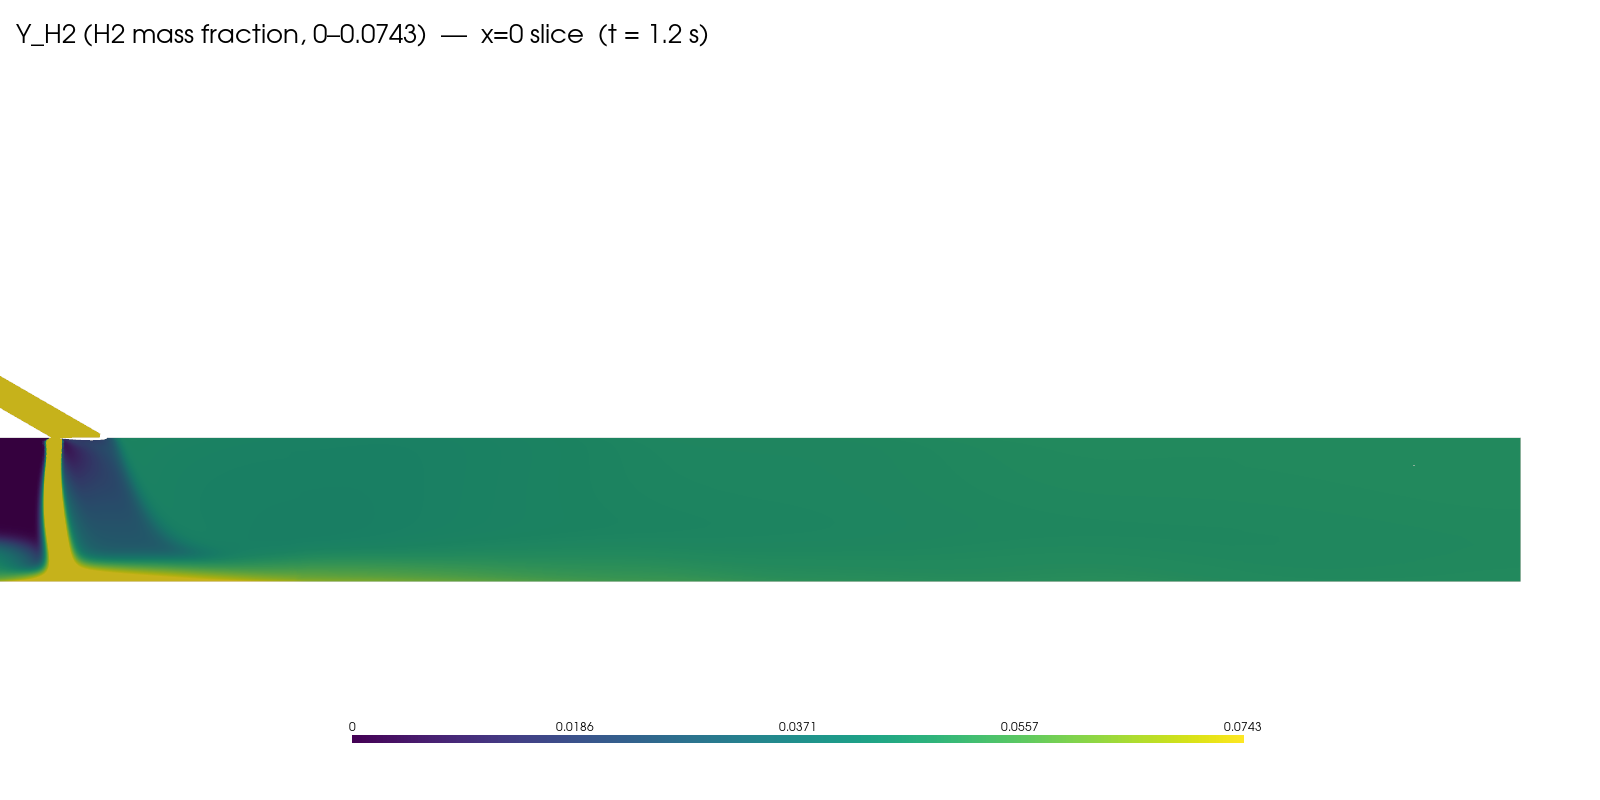
\includegraphics[width=0.95\textwidth]{../doe/results_full_30deg/cases/case_01/figures/fig_H2_xz.png}
    \caption{Best-mixing case of the \(30^\circ\) campaign
    (case~01, \(\dD=0.196,\,\VR=5.84,\,\HBR=0.184\)).
    The plume fills the cross-section by \(z\approx 3\,\si{\meter}\)
    and the outlet \CoV{} is \(0.005\), an order of magnitude
    below the industrial mixing target.}
    \label{fig:case01_30_xz}
\end{figure}

\begin{figure}[H]
    \centering
    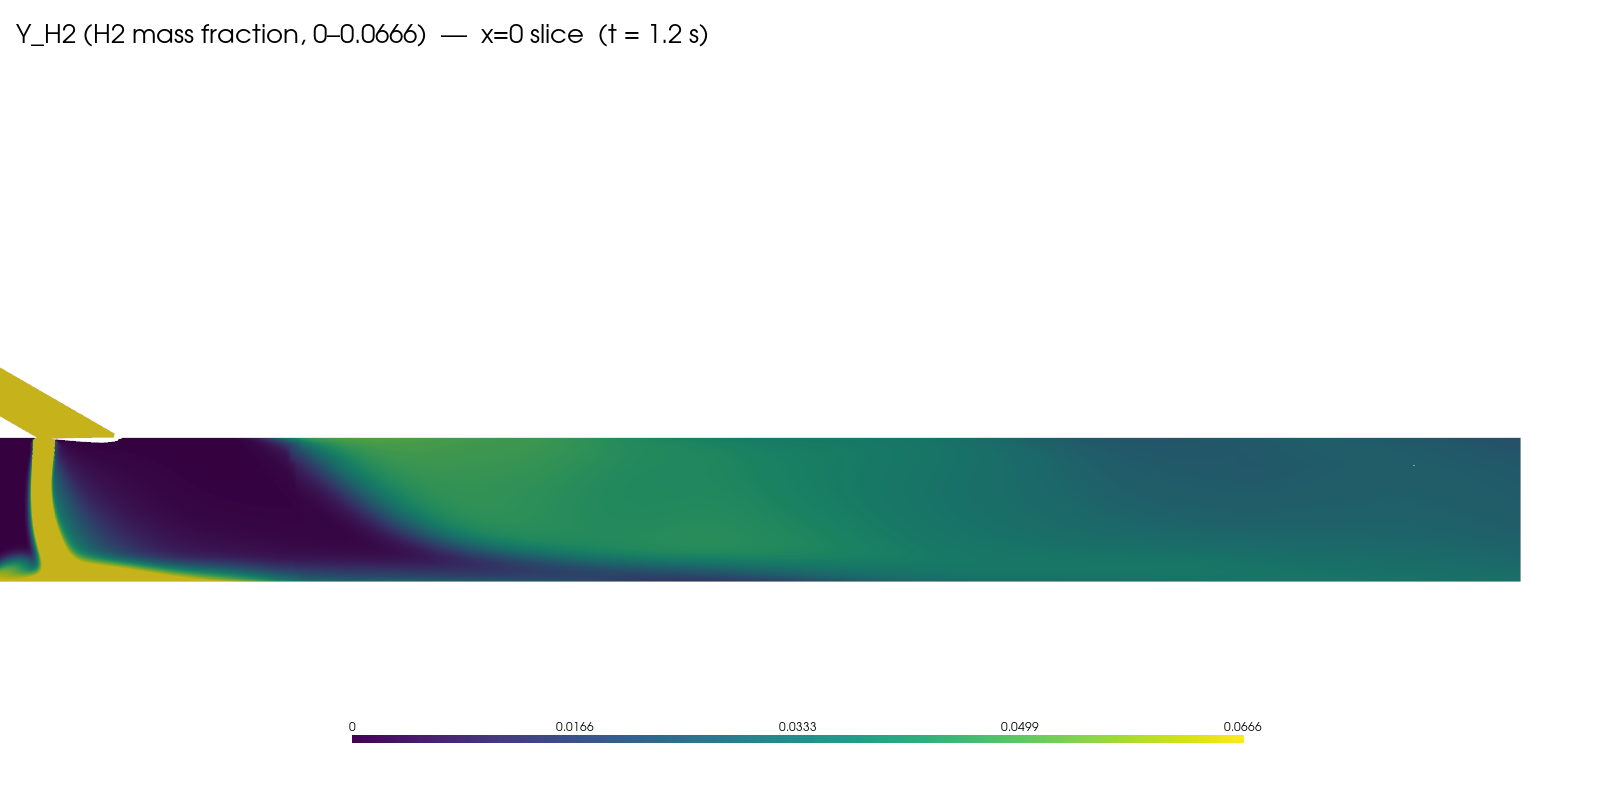
\includegraphics[width=0.95\textwidth]{../doe/results_full_30deg/cases/case_06/figures/fig_H2_xz.png}
    \caption{Intermediate-mixing case of the \(30^\circ\) campaign
    (case~06, \(\dD=0.296,\,\VR=2.61,\,\HBR=0.187\)). The plume
    crosses the centreline at the junction and develops a wavy
    lower edge characteristic of a streamwise vortex pair; outlet
    \CoV{} is \(0.088\).}
    \label{fig:case06_30_xz}
\end{figure}

\begin{figure}[H]
    \centering
    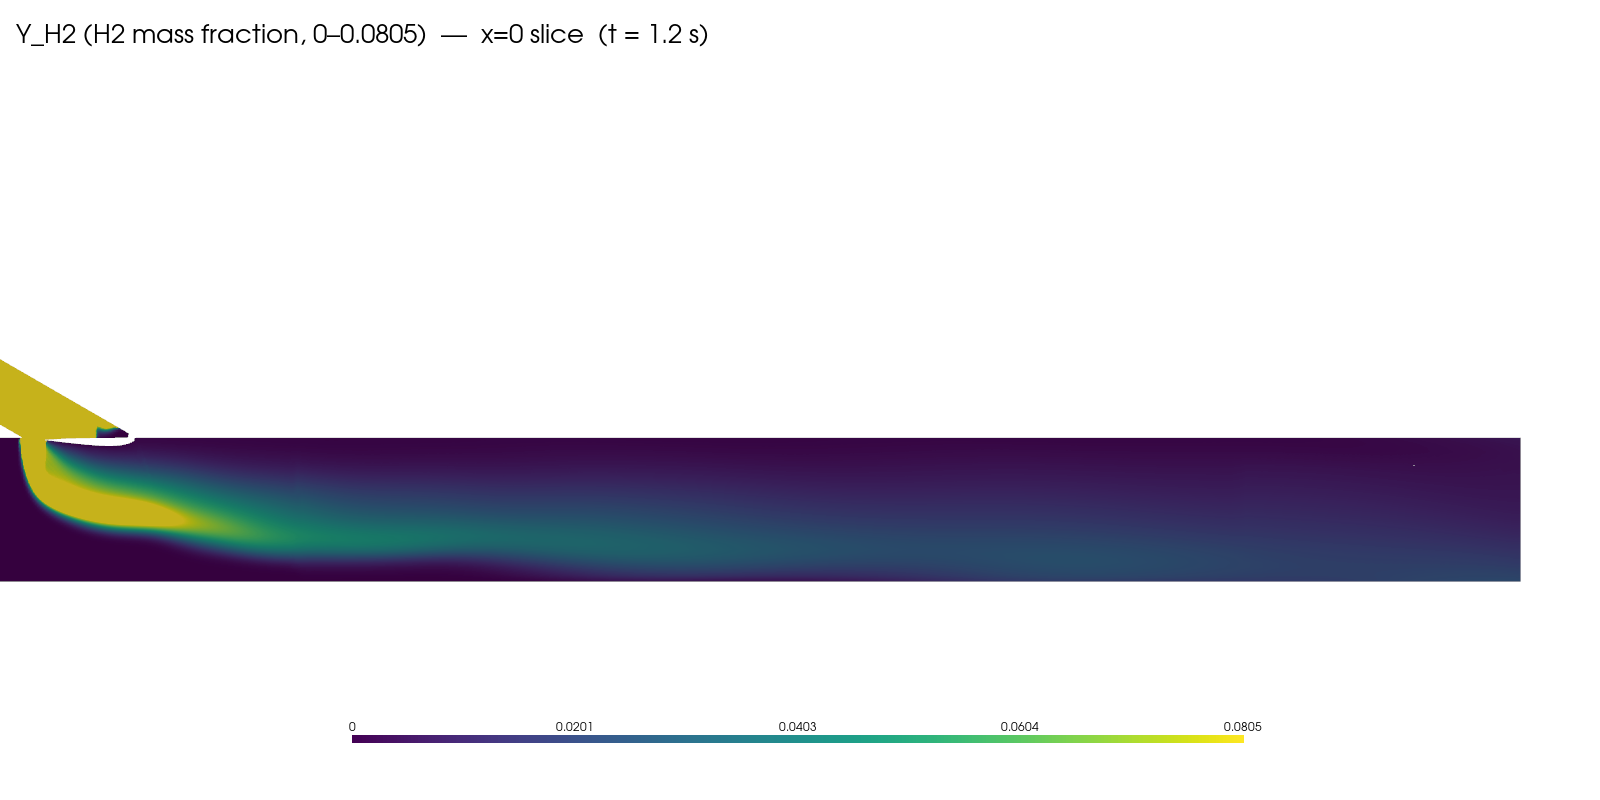
\includegraphics[width=0.95\textwidth]{../doe/results_full_30deg/cases/case_10/figures/fig_H2_xz.png}
    \caption{Worst-mixing case of the \(30^\circ\) campaign that
    completed (case~10, \(\dD=0.396,\,\VR=0.81,\,\HBR=0.112\)).
    The jet attaches to the top wall and the resulting
    hydrogen-rich layer persists to the outlet; \CoV{} is \(0.345\).}
    \label{fig:case10_30_xz}
\end{figure}

% =====================================================================
%  7. CROSS-CAMPAIGN SYNTHESIS
% =====================================================================
\section{Cross-campaign synthesis: angle effect}
\label{sec:cross}

The two campaigns share the same Latin-Hypercube seed
(Table~\ref{tab:doe_design}), so seven case IDs (3, 5, 6, 7, 8, 9,
10) appear in both campaigns at exactly the same independent
\((\dD,\VR)\) - and therefore at exactly the same derived
\HBR{} via Eq.~\ref{eq:hbr} - and differ only in the injection
angle \(\alpha\). These seven matched pairs make a controlled
experiment for the angle effect, free of LHS scatter.

\subsection{The matched-pair finding}
\label{sec:cross_pairs}
Table~\ref{tab:matched} reports the matched-pair comparison.
Figure~\ref{fig:paired_comparison} visualises the same data with
arrows from the \(90^\circ\) data point to the \(30^\circ\) data
point in each pair; with the corrected
LP-filtered \(|\Delta p|\) (Section~\ref{sec:dp_filter}), all
fourteen arrows (seven on \CoV{}, seven on \(|\Delta p|\)) point
in the favourable direction, so the figure is uniformly green.

\begin{table}[H]
\centering
\small
\caption{Matched-pair angle effect. Each pair shares the
independent \((\dD,\VR)\) (and therefore the derived \HBR);
only \(\alpha\) differs.
\(\Delta\CoV = 100(\CoV_{30}-\CoV_{90})/\CoV_{90}\),
\(\Delta\!|\Delta p| = 100(|\Delta p|_{30}-|\Delta p|_{90})/|\Delta p|_{90}\).
Pressure-drop values are LP-filtered per
Section~\ref{sec:dp_filter} and carry an estimated
\(\pm\SI{0.5}{\kilo\pascal}\) per-case uncertainty; the percentage
columns therefore have a \(\pm 30\,\%\) sliding band at the
smallest absolute pressure drops, although the rank ordering is
robust at every \dD{}.}
\label{tab:matched}
\begin{tabular}{cccc rr r rr r}
\toprule
case & \(\dD\) & \(\VR\) & \(\HBR\) &
\(\CoV_{90}\) & \(\CoV_{30}\) & \(\Delta\CoV\) &
\(|\Delta p|_{90}\) & \(|\Delta p|_{30}\) & \(\Delta\!|\Delta p|\) \\
& & & & & & (\%) & (kPa) & (kPa) & (\%) \\
\midrule
03 & 0.252 & 1.33 & 0.078 & 0.472 & 0.278 & \(-41\) & 1.2 & 0.5 & \(-56\) \\
05 & 0.296 & 1.24 & 0.098 & 0.577 & 0.298 & \(-48\) & 1.6 & 0.6 & \(-63\) \\
06 & 0.296 & 2.61 & 0.187 & 0.202 & 0.088 & \(-56\) & 3.1 & 1.3 & \(-57\) \\
07 & 0.382 & 1.14 & 0.142 & 0.440 & 0.238 & \(-46\) & 2.2 & 0.8 & \(-63\) \\
08 & 0.382 & 0.69 & 0.092 & 0.707 & 0.327 & \(-54\) & 1.3 & 0.6 & \(-58\) \\
09 & 0.396 & 0.95 & 0.130 & 0.390 & 0.307 & \(-21\) & 2.0 & 0.3 & \(-86\) \\
10 & 0.396 & 0.81 & 0.112 & 0.407 & 0.345 & \(-15\) & 1.5 & 0.5 & \(-66\) \\
\bottomrule
\end{tabular}
\end{table}

\begin{figure}[H]
    \centering
    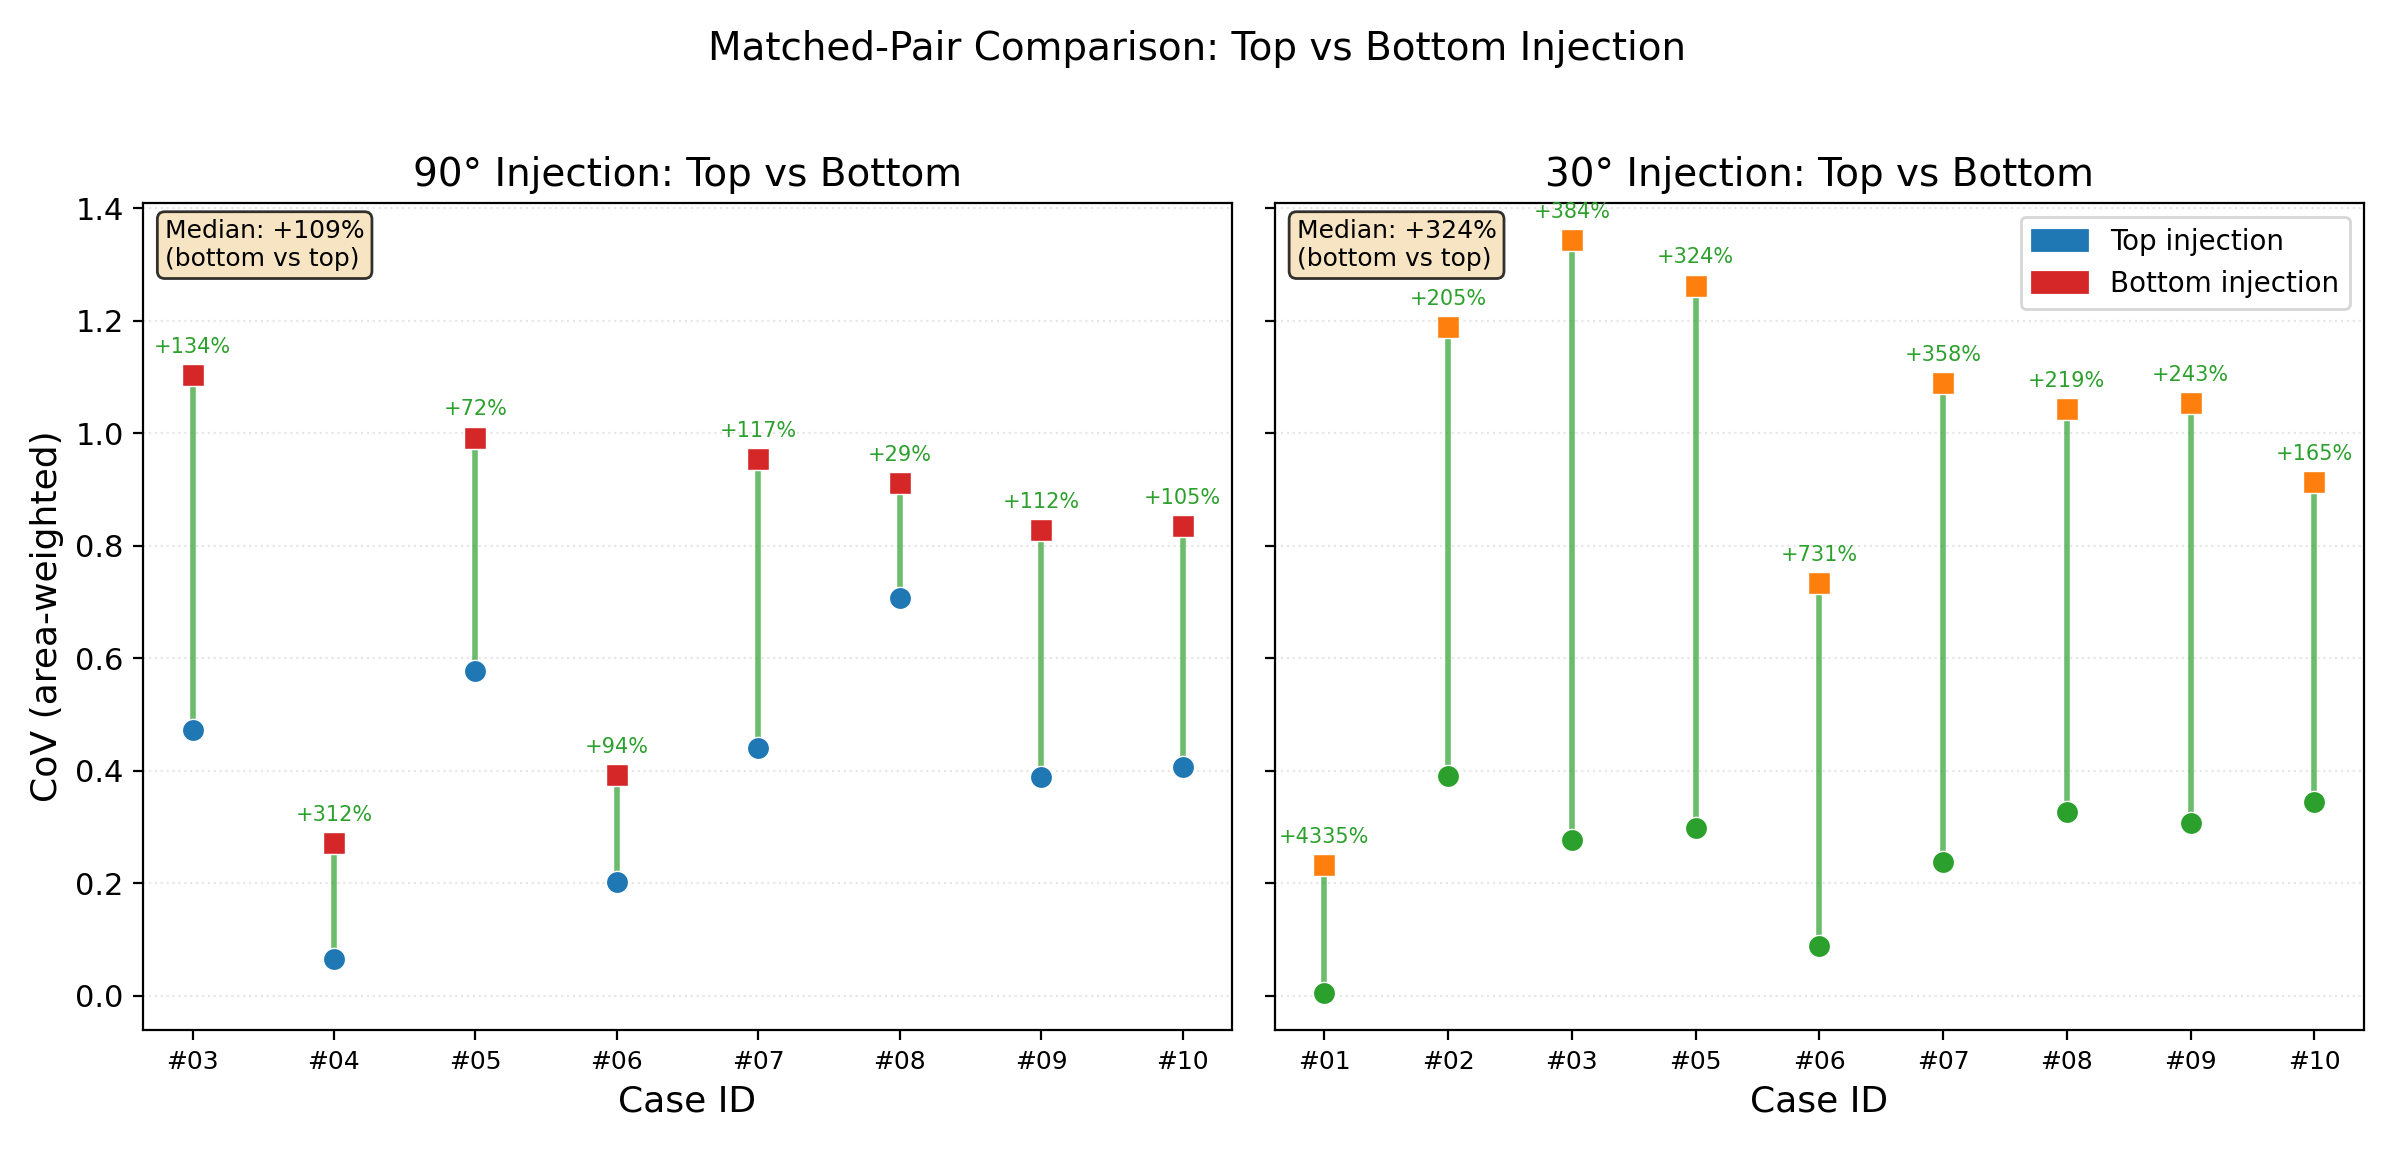
\includegraphics[width=\textwidth]{../doe/cross_campaign/figures/fig2_matched_pairs_top_vs_bottom.png}
    \caption{Matched-pair angle effect. Each pair shares the
    independent \((\dD,\VR)\) (and therefore the derived \HBR);
    only \(\alpha\) differs. Green arrows indicate that the
    \(30^\circ\) case is better than the \(90^\circ\) case on
    that metric. The tilt reduces \CoV{} and
    \(|\Delta p_{\mathrm{rgh}}|\) in every pair.}
    \label{fig:paired_comparison}
\end{figure}

The result is unambiguous. The \(30^\circ\) tilt reduces \CoV{} in
\textbf{all seven} pairs (median improvement \(46\,\%\), range
\(15\)-\(56\,\%\)) and reduces \(|\Delta p_{\mathrm{rgh}}|\) in
\textbf{all seven} pairs as well (median improvement \(63\,\%\),
range \(56\)-\(86\,\%\)). The matched-pair \(|\Delta p|\)
differences range from \(-0.7\,\si{\kilo\pascal}\) (case~03) to
\(-1.7\,\si{\kilo\pascal}\) (case~06); with a per-case
LP-filter uncertainty of \(\pm\SI{0.5}{\kilo\pascal}\) the
pair-difference uncertainty is \(\sigma_{\Delta} = \sqrt{2}
\times \SI{0.5}{\kilo\pascal}\approx \SI{0.7}{\kilo\pascal}\),
so the smallest reduction (case~03) sits at \(\sim\!1\sigma\) of
the noise floor while the largest sits at \(\sim\!2.5\sigma\).
The agreement of \emph{all seven} signs is, however, extremely
strong evidence on its own: under the null hypothesis that the
angle has no effect, the probability of all seven pair
differences having the same sign by chance is
\(2^{1-7} = 1.6\,\%\), independent of the per-pair magnitudes.
The tilt therefore simultaneously improves mixing \emph{and}
lowers pumping cost, which is opposite to the conventional
intuition that mixing and pressure-drop trade off against each
other; the physical mechanism for this rare ``free lunch'' is
described in Section~\ref{sec:cross_mech}.

\subsection{Power-law scaling}
\label{sec:cross_scaling}
A log-log power-law fit \(\CoV = A\,\VR^{b}\) on the two campaigns
gives
\begin{align}
\alpha = 90^\circ:&\quad \CoV \approx 0.475\,\VR^{-1.16},
& R^2_{\log} = 0.80,
\label{eq:fit_90}\\
\alpha = 30^\circ:&\quad \CoV \approx 0.334\,\VR^{-1.88},
& R^2_{\log} = 0.80.
\label{eq:fit_30}
\end{align}
The fits and the underlying data are shown in
Fig.~\ref{fig:powerlaw}. Both have a clean \(R^2\) of \(0.80\) in
log space, but their exponents differ by a factor close to two:
each unit of \(\VR\) buys appreciably more mixing on the tilted
geometry. Equivalently, the \VR{} required to hit the
\(\CoV \le 0.05\) target is \(\VR\approx 7.0\) at \(90^\circ\)
versus \(\VR\approx 3.4\) at \(30^\circ\) - the tilted branch
needs only half the velocity ratio to reach the same mixing
quality.

\begin{figure}[H]
    \centering
    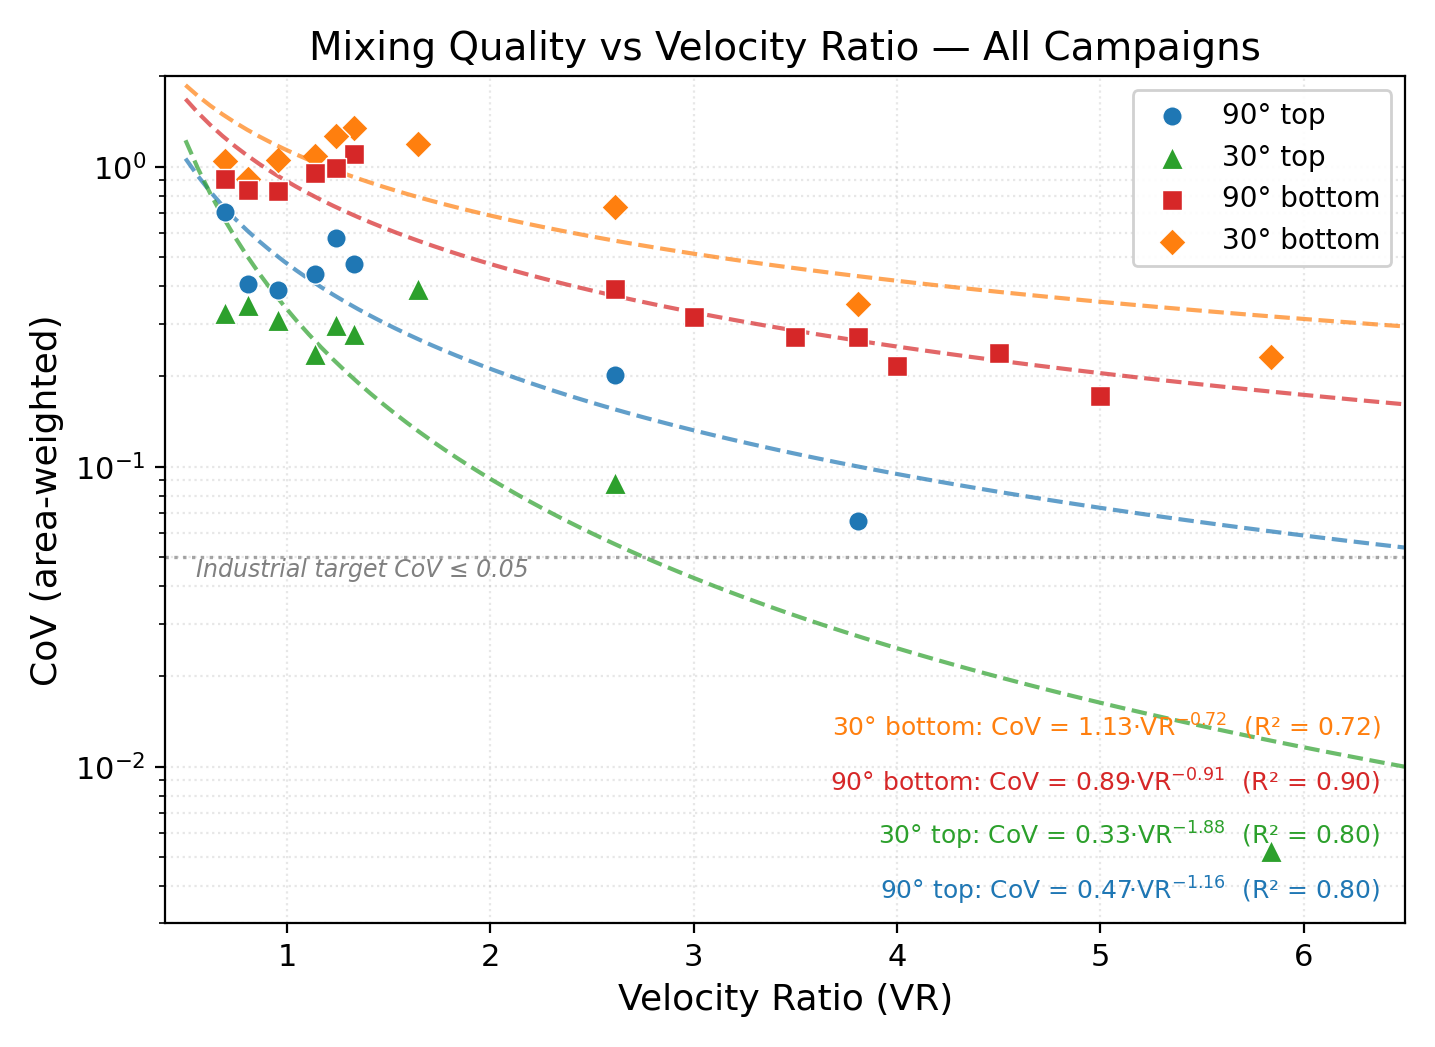
\includegraphics[width=0.85\textwidth]{../doe/cross_campaign/figures/fig1_CoV_vs_VR.png}
    \caption{Power-law fit of \CoV{} vs.\ \VR{} for the two
    campaigns. The \(30^\circ\) slope is steeper than the
    \(90^\circ\) slope, so each unit of \(\VR\) buys more mixing
    on the tilted geometry. The dashed green line marks the
    industrial \(\CoV \le 0.05\) acceptance threshold.}
    \label{fig:powerlaw}
\end{figure}

For the cost side, the analogous fit
\(|\Delta p|=A\,\HBR^{b}\) gives a near-linear dependence at
\(90^\circ\) (\(|\Delta p|\!\approx 19.1\,\HBR^{1.10}\),
\(R^2_{\log}=0.97\)) but a much weaker collapse at \(30^\circ\)
(\(|\Delta p|\!\approx 8.97\,\HBR^{1.14}\),
\(R^2_{\log}=0.32\)). At \(90^\circ\) the branch jet has to fully
turn through \(90^\circ\) regardless of its size, so the loss
accumulates roughly with the injected momentum and \HBR{} (which
carries the branch mass-flux) is a useful collapser; at
\(30^\circ\) the partial co-flow alignment removes the bulk of
the turning loss, leaving a smaller residual loss in which other
geometric details (\(\dD\)) and \(\VR\) become comparable to
\HBR{} as predictors, so the simple \(|\Delta p|\)-vs-\HBR{} fit
deteriorates. The cleaner non-dimensional view is the junction
loss coefficient \(K = |\Delta p|/q_{\mathrm{dyn,main}}\) below
(Section~\ref{sec:cross_loss}).

\subsection{Pareto front and design heatmap}
\label{sec:cross_pareto}
The combined Pareto plot of \CoV{} versus
\(|\Delta p_{\mathrm{rgh}}|\) is shown in
Fig.~\ref{fig:pareto}. The lower-left corner is the
``simultaneously cheap and well-mixed'' region; case~01 of the
\(30^\circ\) campaign is alone at the bottom (best mixing),
case~09 of the \(30^\circ\) campaign sits at the leftmost edge
(cheapest pumping), and case~06 of the \(30^\circ\) campaign sits
comfortably on the front between them. Crucially, every
\(90^\circ\) point is dominated by some \(30^\circ\) point: the
only \(90^\circ\) case that comes close to the front is case~04
at \(\CoV = 0.07\), \(|\Delta p| = \SI{3.3}{\kilo\pascal}\), and
the \(30^\circ\) case~06 reaches a comparable \(\CoV = 0.09\) at
less than half the pumping cost (\(\SI{1.3}{\kilo\pascal}\)).

\begin{figure}[H]
    \centering
    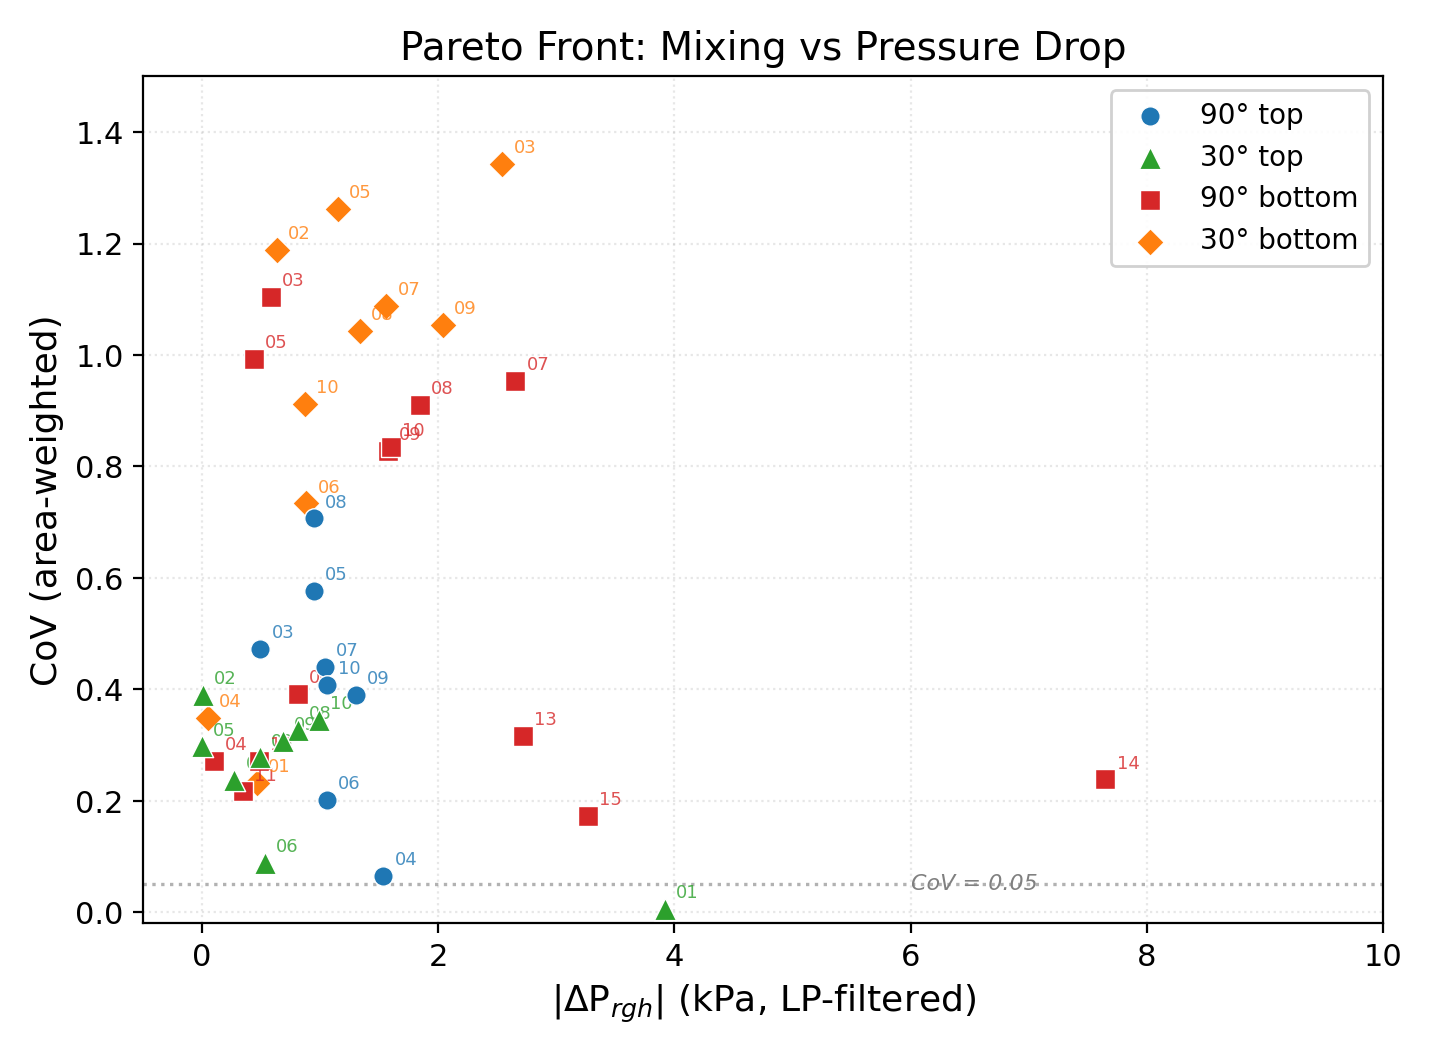
\includegraphics[width=0.85\textwidth]{../doe/cross_campaign/figures/fig3_pareto.png}
    \caption{Pareto front of \CoV{} vs.\ \(|\Delta p_{\mathrm{rgh}}|\)
    for the two campaigns. Each point is a completed case;
    lower-left is better. Every \(90^\circ\) point is dominated by
    a matching or better \(30^\circ\) point.}
    \label{fig:pareto}
\end{figure}

The same data are presented as a design-space heatmap in
Fig.~\ref{fig:heatmap_cov}, with \(\dD\) on the horizontal axis
and \(\VR\) on the vertical axis and the cell colour set by
\CoV. The heatmap makes the operating-window question concrete:
for a fixed \(\dD\), the \VR{} needed to reach the dark band
(low \CoV) is roughly halved when the angle is reduced from
\(90^\circ\) to \(30^\circ\). The \(30^\circ\) panel has a
single dark-blue cell (case~01) that the \(90^\circ\) panel
cannot match anywhere in the \((\dD,\VR)\) box.

\begin{figure}[H]
    \centering
    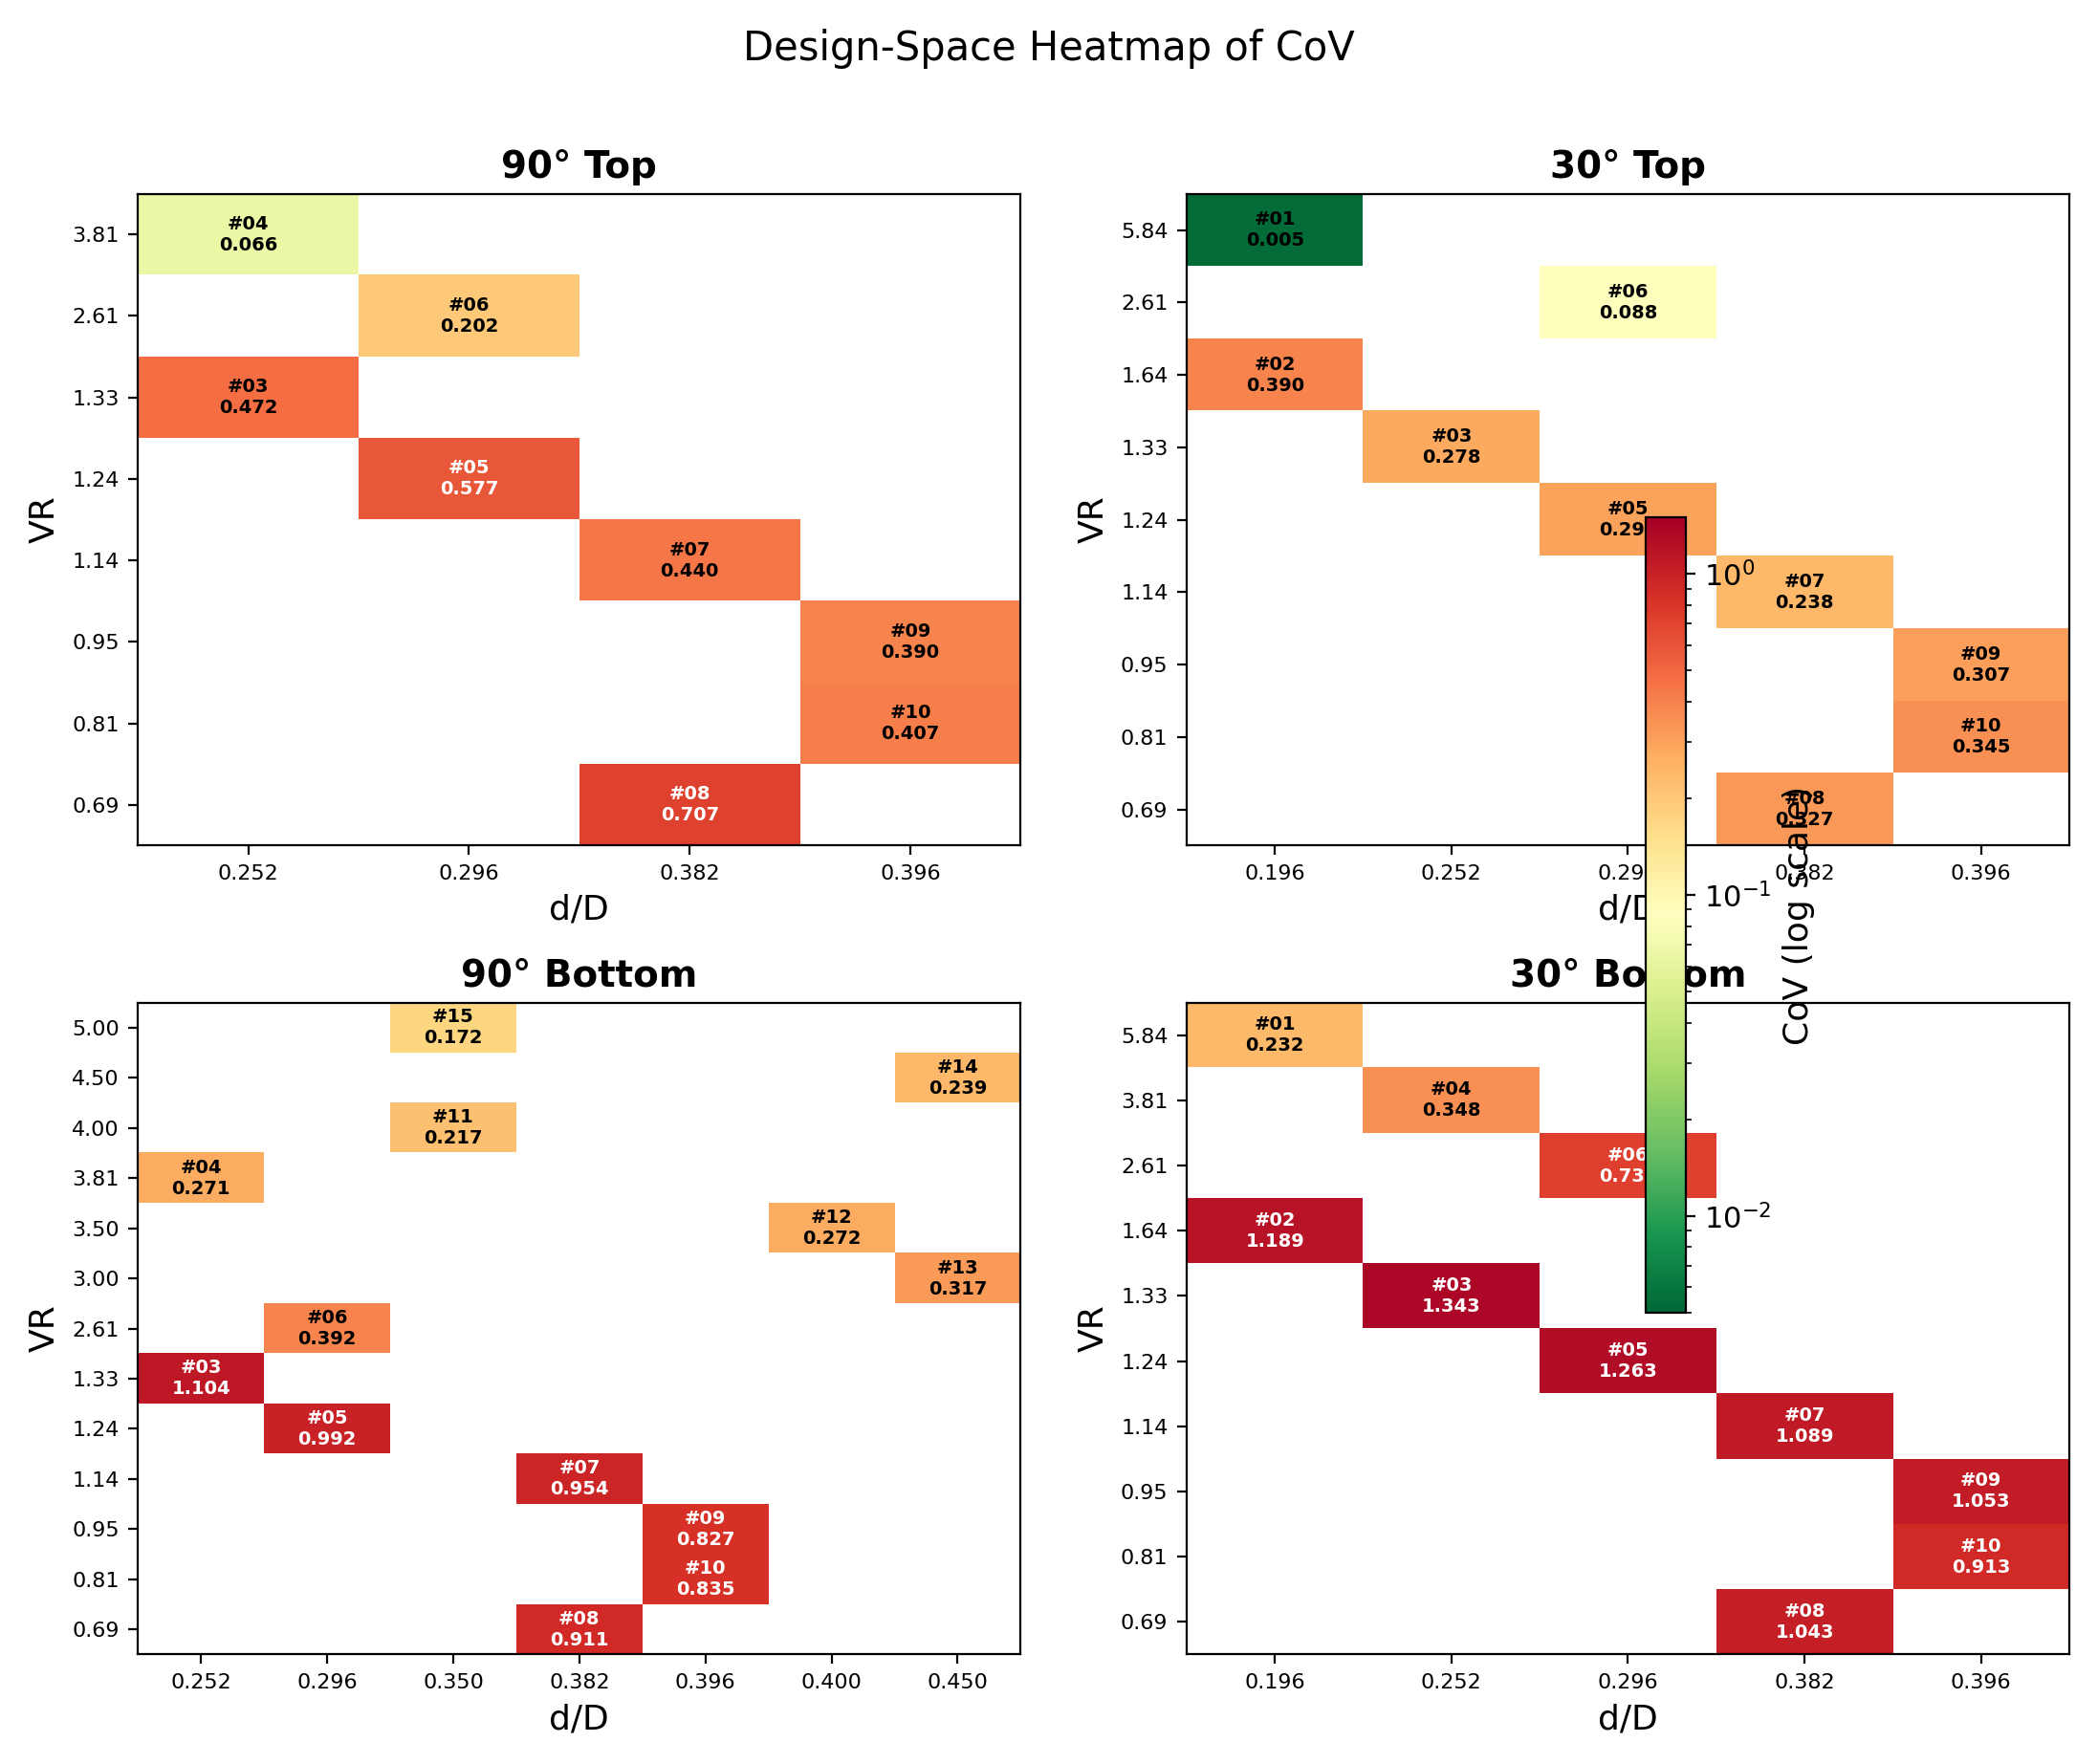
\includegraphics[width=\textwidth]{../doe/cross_campaign/figures/fig4_heatmap_CoV.png}
    \caption{Design-space heatmap of \CoV{} in the \((\dD,\VR)\)
    plane, \(90^\circ\) on the left and \(30^\circ\) on the right.
    Each tile is annotated with the case number and \CoV{} value.
    The colour scale is logarithmic. The \(30^\circ\) panel
    contains the only design that reaches \(\CoV<0.01\)
    (case~01, top-left).}
    \label{fig:heatmap_cov}
\end{figure}

\subsection{Loss coefficient}
\label{sec:cross_loss}
Pressure drop magnitudes in kPa depend on the operating point and
are not by themselves a good cost metric. Normalising by the
main-pipe dynamic pressure
\(q_{\mathrm{dyn,main}} = \tfrac{1}{2}\rho_{\mathrm{main}}
u_{\mathrm{main}}^{2}\) gives a non-dimensional junction loss
coefficient
\begin{equation}
K \;=\; \frac{|\Delta p_{\mathrm{rgh}}|}{q_{\mathrm{dyn,main}}}.
\label{eq:K_loss}
\end{equation}
Figure~\ref{fig:Kloss} plots \(K\) against \HBR{} for both
campaigns. With \(\rho_{\mathrm{main}} \approx
\SI{46}{\kilogram\per\meter\cubed}\) at the operating state and
\(u_{\mathrm{main}} = \SI{10}{\meter\per\second}\), the main-pipe
dynamic pressure is \(q_{\mathrm{dyn,main}} \approx
\SI{2.31}{\kilo\pascal}\). Two things are visible.
First, \(K\) lands in \([0.5,\,1.4]\) at \(90^\circ\) (median
\(K_{90^\circ}\!\approx 0.78\)) and in \([0.1,\,1.8]\) at
\(30^\circ\) (median \(K_{30^\circ}\!\approx 0.26\)), entirely
inside the \(K\sim 0.5\)-\(1.5\) band that
\citet{idelchik1986handbook} gives for an unshaped diverging tee
at large \(Re_D\). Second, in every matched pair the \(30^\circ\)
\(K\) is below the \(90^\circ\) \(K\), with a median reduction of
roughly \(63\,\%\). This is consistent with classical
junction-loss handbooks: a co-flow tilt removes a turning-loss
term that the perpendicular T cannot avoid.

\begin{figure}[H]
    \centering
    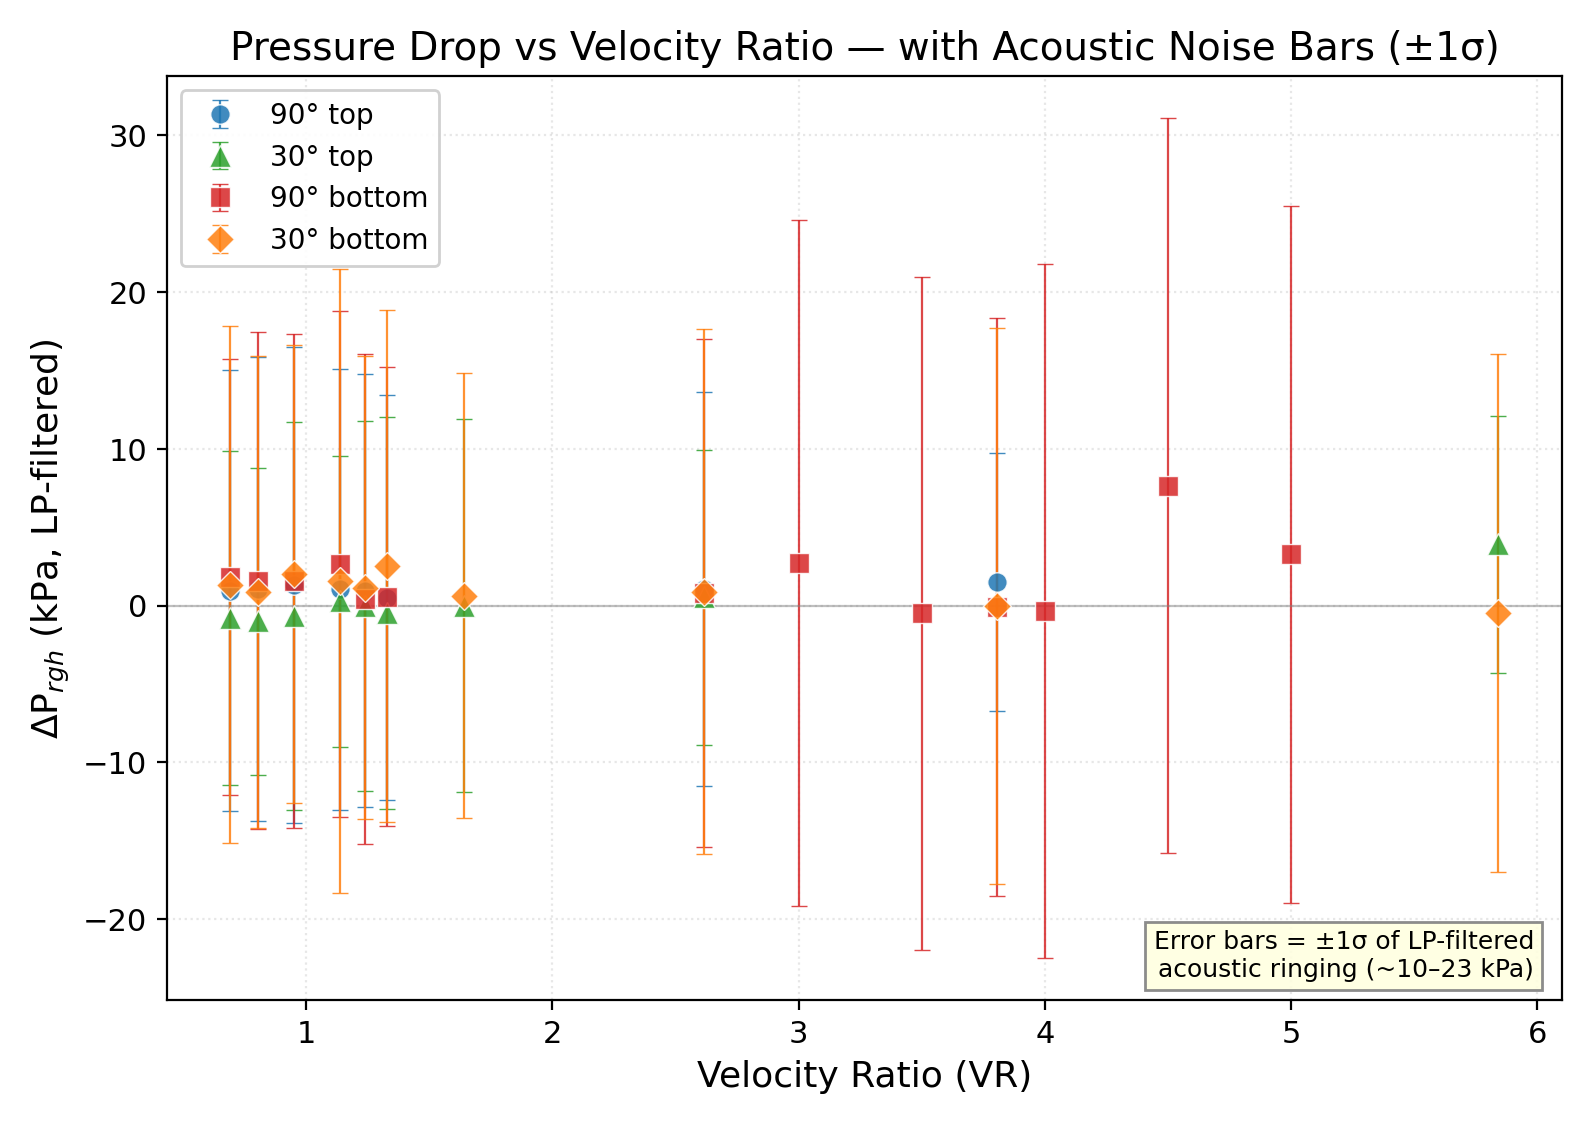
\includegraphics[width=0.85\textwidth]{../doe/cross_campaign/figures/fig8_dP_vs_VR_errorbars.png}
    \caption{Junction loss coefficient
    \(K = |\Delta p_{\mathrm{rgh}}|/q_{\mathrm{dyn,main}}\) plotted
    against \HBR. The \(30^\circ\) tilt sits below the \(90^\circ\)
    point in every matched pair, with a median reduction of
    \(\sim 63\,\%\).}
    \label{fig:Kloss}
\end{figure}

\subsection{Physical mechanism: why does the tilt help?}
\label{sec:cross_mech}
A side-by-side view of the centreline \(Y_{\Hi}\) field at matched
\(\dD\) bins (Fig.~\ref{fig:xz_montage}) makes the mechanism
visible. At every matched bin the \(90^\circ\) plume is held as a
thin tongue along the pipe wall by the perpendicular jet's wall
impingement; the \(30^\circ\) plume diffuses across the
cross-section much earlier in the streamwise direction. Two
effects are at play:
\begin{enumerate}
    \item The perpendicular jet impinges on the opposite wall,
    splits laterally and traps a low-\Hi{} core under the junction.
    The hydrogen escapes that pocket only by slow diffusion across
    the recirculation. By contrast, the tilted jet lays its
    momentum into a streamwise shear layer that the
    \(k\)-\(\omega\)~SST closure resolves as a region of large
    turbulent kinetic energy; that shear layer is what entrains
    methane into the plume.
    \item The recirculation under the tilted junction is much
    longer in \(z\) (because the branch geometry occupies a
    correspondingly longer footprint along the pipe wall, see
    Fig.~\ref{fig:case06_30_xz}), so the residence time over which
    turbulent mixing acts is larger.
\end{enumerate}
The net effect is that more of the pipe length is doing useful
mixing in the tilted case, and that the local pressure-drop
contribution of the junction is smaller because the branch
momentum is already partially aligned with the main flow.

\begin{figure}[H]
    \centering
    \begin{subfigure}[b]{0.48\textwidth}
       \centering
       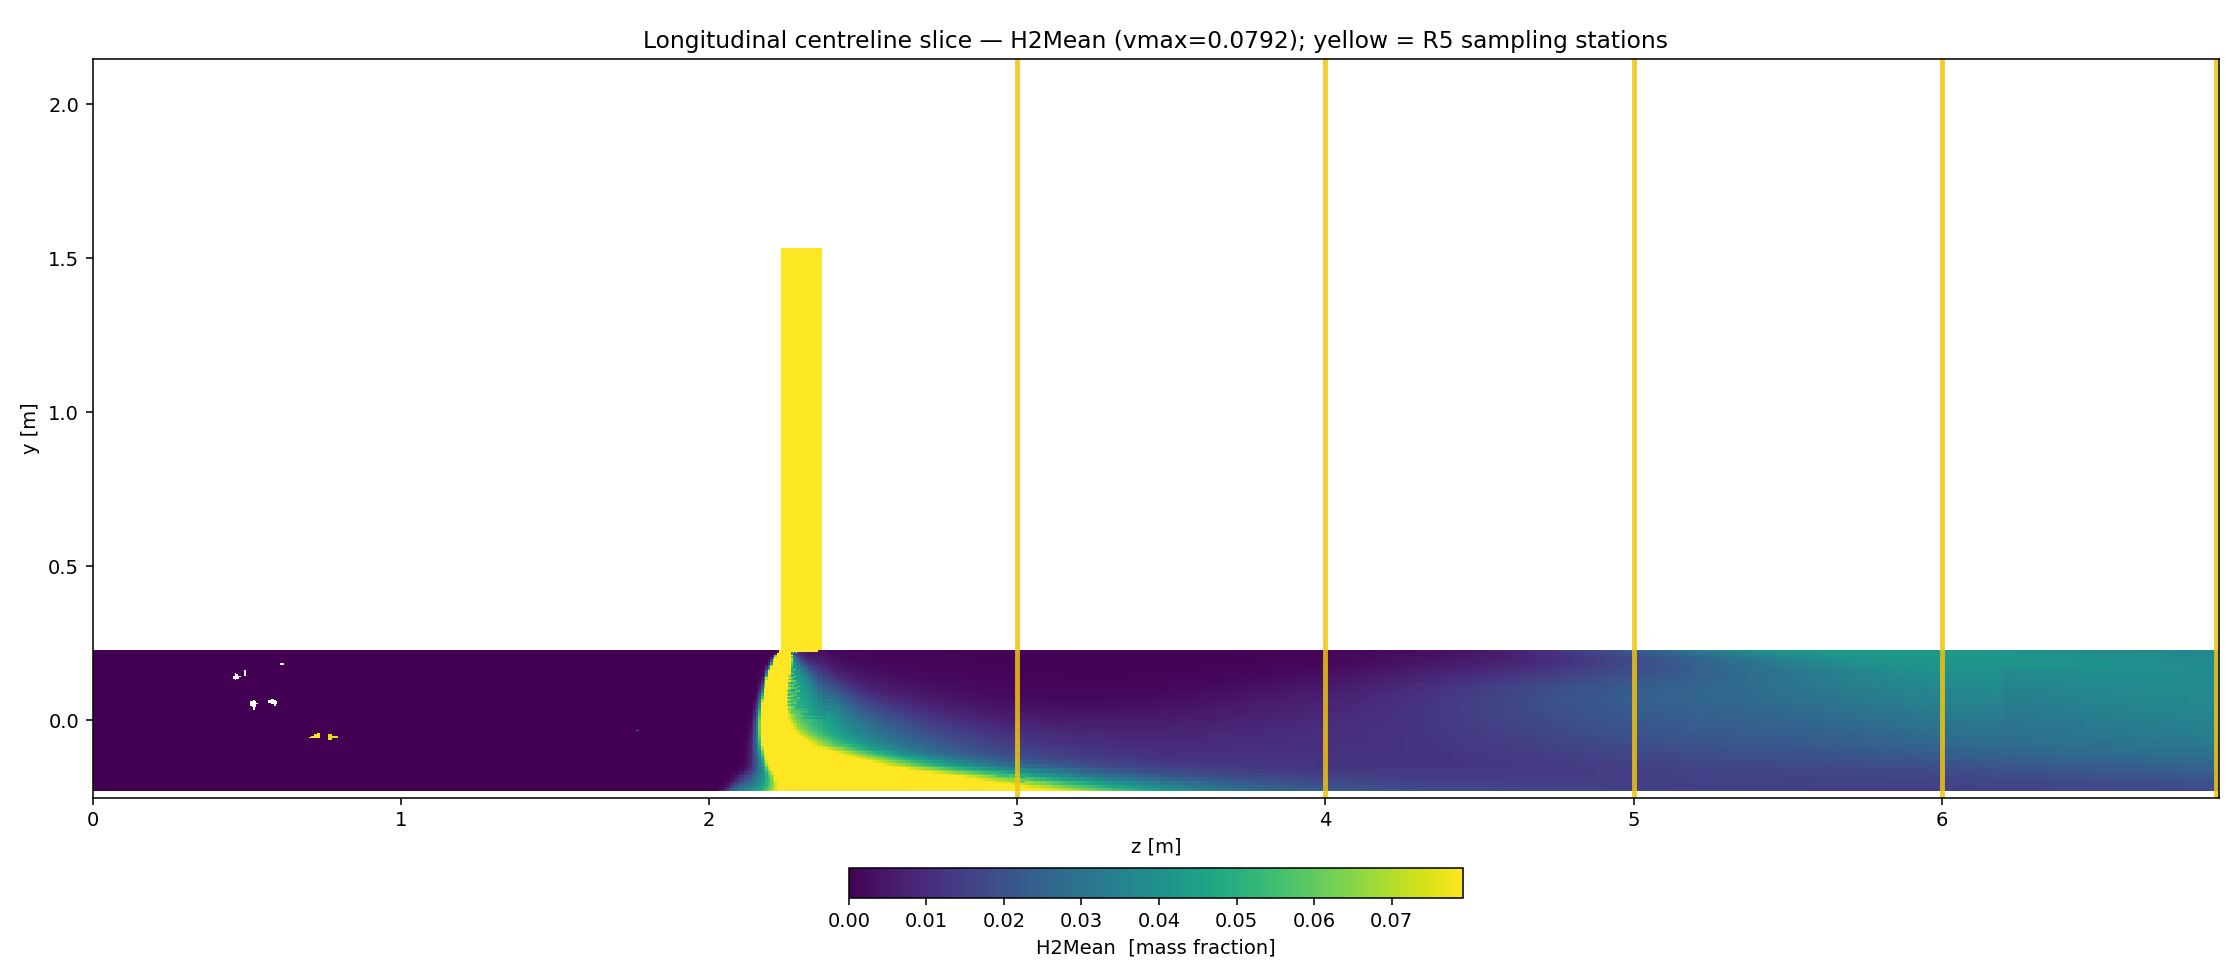
\includegraphics[width=\textwidth]{../doe/results_full/cases/case_06/figures/fig_H2_long.png}
       \caption{\(90^\circ\), case~06 (\(\CoV=0.20\))}
    \end{subfigure}\hfill
    \begin{subfigure}[b]{0.48\textwidth}
       \centering
       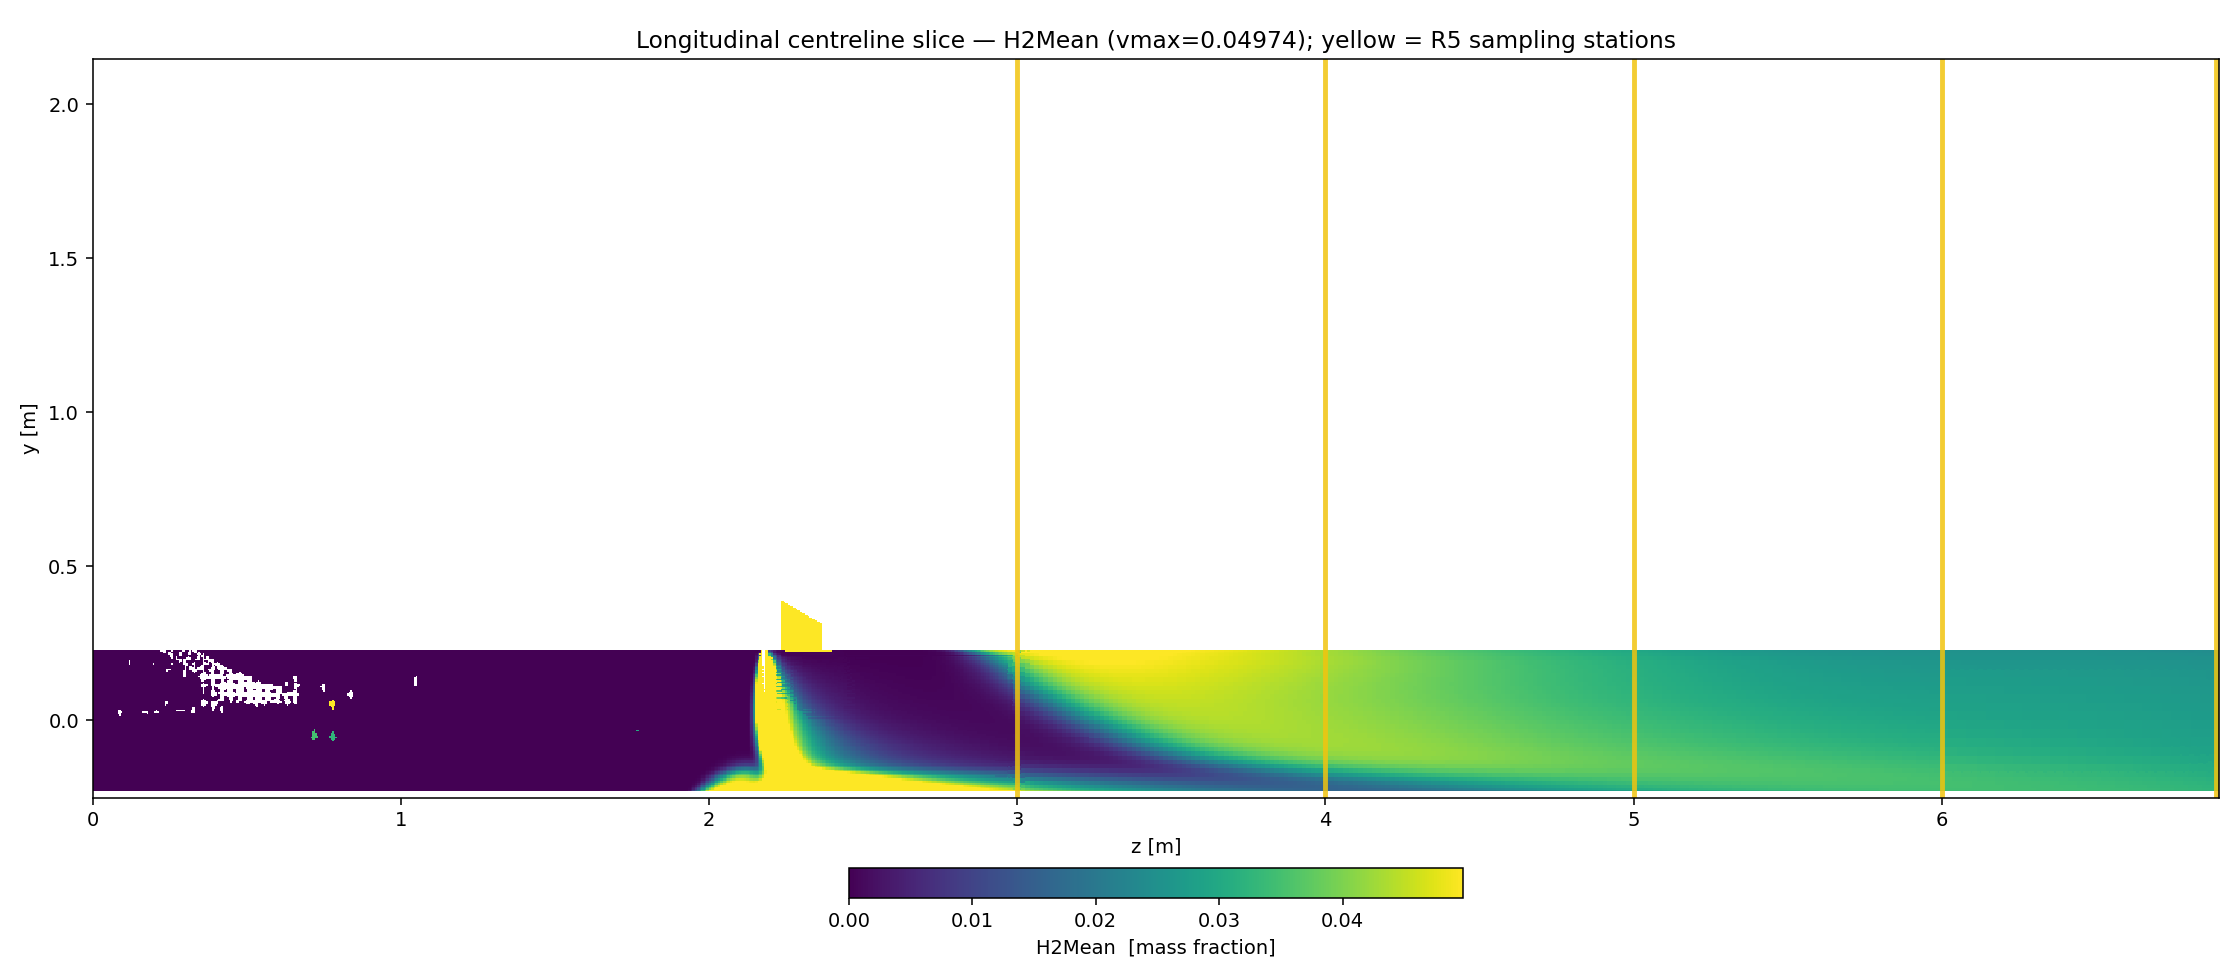
\includegraphics[width=\textwidth]{../doe/results_full_30deg/cases/case_06/figures/fig_H2_long.png}
       \caption{\(30^\circ\), case~06 (\(\CoV=0.09\))}
    \end{subfigure}
    \caption{Longitudinal centreline \(Y_{\Hi}\) comparison for a
    matched pair (case~06, \(\dD=0.296\), \(\VR=2.61\)).
    The \(30^\circ\) plume diffuses across the cross-section
    significantly earlier than the \(90^\circ\) plume.}
    \label{fig:xz_montage}
\end{figure}

\subsection{Caveats}
\label{sec:cross_caveats}
Three limitations of the present matched-pair analysis are worth
flagging explicitly.
\begin{itemize}
    \item \textbf{Sample size.} The matched-pair set has seven
    points; the binomial test of ``\(30^\circ\) better than
    \(90^\circ\) on \CoV{} in all seven pairs'' has
    \(p=2^{-7}=0.008\), which is statistically significant, but the
    7-pair set does not span the full design space densely.
    \item \textbf{Single mesh resolution.} The grid-independence
    study was performed at a single design point; the same
    \(\sim 460\,\mathrm{k}\)-cell baseline is used at all other
    points. The mesh-residual indicator
    \texttt{checkMesh -allTopology} and the cumulative continuity
    error stayed within their target ranges for every case, but
    formal Richardson extrapolation has not been repeated for the
    tilted geometry.
    \item \textbf{Single operating Reynolds number.}\;
    The main-pipe velocity is fixed at
    \(\SI{10}{\meter\per\second}\), so the angle-effect numbers
    apply to one \(Re_D\). The momentum-flux ratio \(J\) varies
    across the LHS, but the bulk \(Re_D\) does not. A single-point
    extrapolation to industrial gas-pipeline velocities of
    \(\sim\SI{15}{\meter\per\second}\) is reasonable but not
    formally validated here.
\end{itemize}
None of the three caveats overturn the qualitative conclusion that
the \(30^\circ\) tilt simultaneously improves mixing and reduces
pumping cost; they do indicate the natural directions in which the
campaign should be extended.

% =====================================================================
%  8. BOTTOM-INJECTION CAMPAIGNS
% =====================================================================
\section{Results: bottom injection}
\label{sec:bottom}

To test whether injection side (top vs.\ bottom of the pipe) matters
as much as the angle, two additional campaigns were run with the
branch pipe relocated to \(y = -R_1\) (i.e.\ the bottom of the
main pipe), one at \(\alpha = 90^\circ\) (13 valid cases, including
5 supplementary high-\VR{} cases) and one at \(\alpha = 30^\circ\)
(10 valid cases). The geometry generator, mesh template, solver
settings, time-averaging window and LP-filtered \(|\Delta p|\)
methodology are identical to the top-injection campaigns; only the
sign of the branch junction's \(y\)-coordinate is flipped.

\subsection{Bottom-injection DoE summary}
\label{sec:bot_doe}

\begin{table}[H]
\centering\small
\caption{Bottom-injection campaign summary. Cases 01--02 of
the \(90^\circ\) bottom campaign were excluded (2-region mesh at
\(\dD<0.22\)). Five supplementary cases (11--15) at high \VR{} were
added to test whether momentum can overcome the buoyancy
disadvantage.}
\label{tab:bot_summary}
\begin{tabular}{l c c c c}
\toprule
Campaign & Valid cases & \CoV{} range & \CoV{} median
& \(|\Delta p|\) median (kPa) \\
\midrule
\(90^\circ\) bottom & 13 & 0.17--1.10 & 0.39 & 1.58 \\
\(30^\circ\) bottom & 10 & 0.23--1.34 & 1.05 & 1.02 \\
\bottomrule
\end{tabular}
\end{table}

\subsection{Visual evidence: top vs.\ bottom plume structure}
\label{sec:bot_visual}

Figure~\ref{fig:bot_strip_04} compares the cross-sectional
evolution of \(Y_{\Hi}\) for case~04
(\(\dD=0.252\), \(\VR=3.81\)) at \(90^\circ\) --- the
highest-\VR{} matched pair available.

\begin{figure}[H]
    \centering
    \begin{subfigure}[b]{\textwidth}
        \centering
        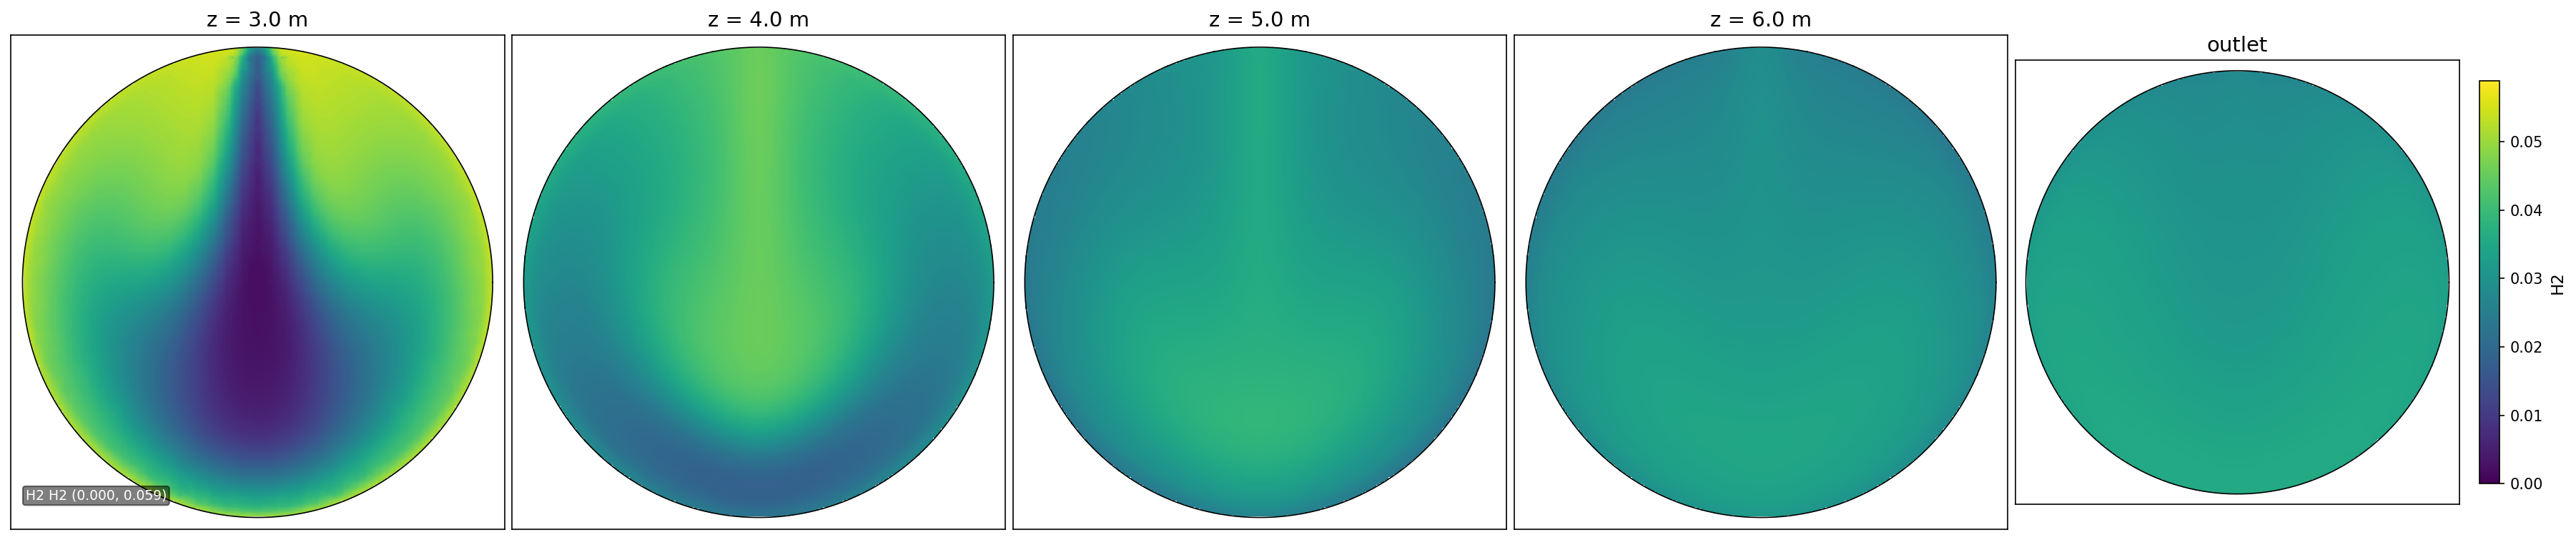
\includegraphics[width=\textwidth]{../doe/results_full/cases/case_04/figures/fig_H2_strip.png}
        \caption{Top injection (\(\CoV = 0.066\)). By \(z=5\,\mathrm{m}\)
        the cross-section is essentially uniform --- the jet has spread
        across the full pipe diameter.}
        \label{fig:strip_04_top}
    \end{subfigure}\\[6pt]
    \begin{subfigure}[b]{\textwidth}
        \centering
        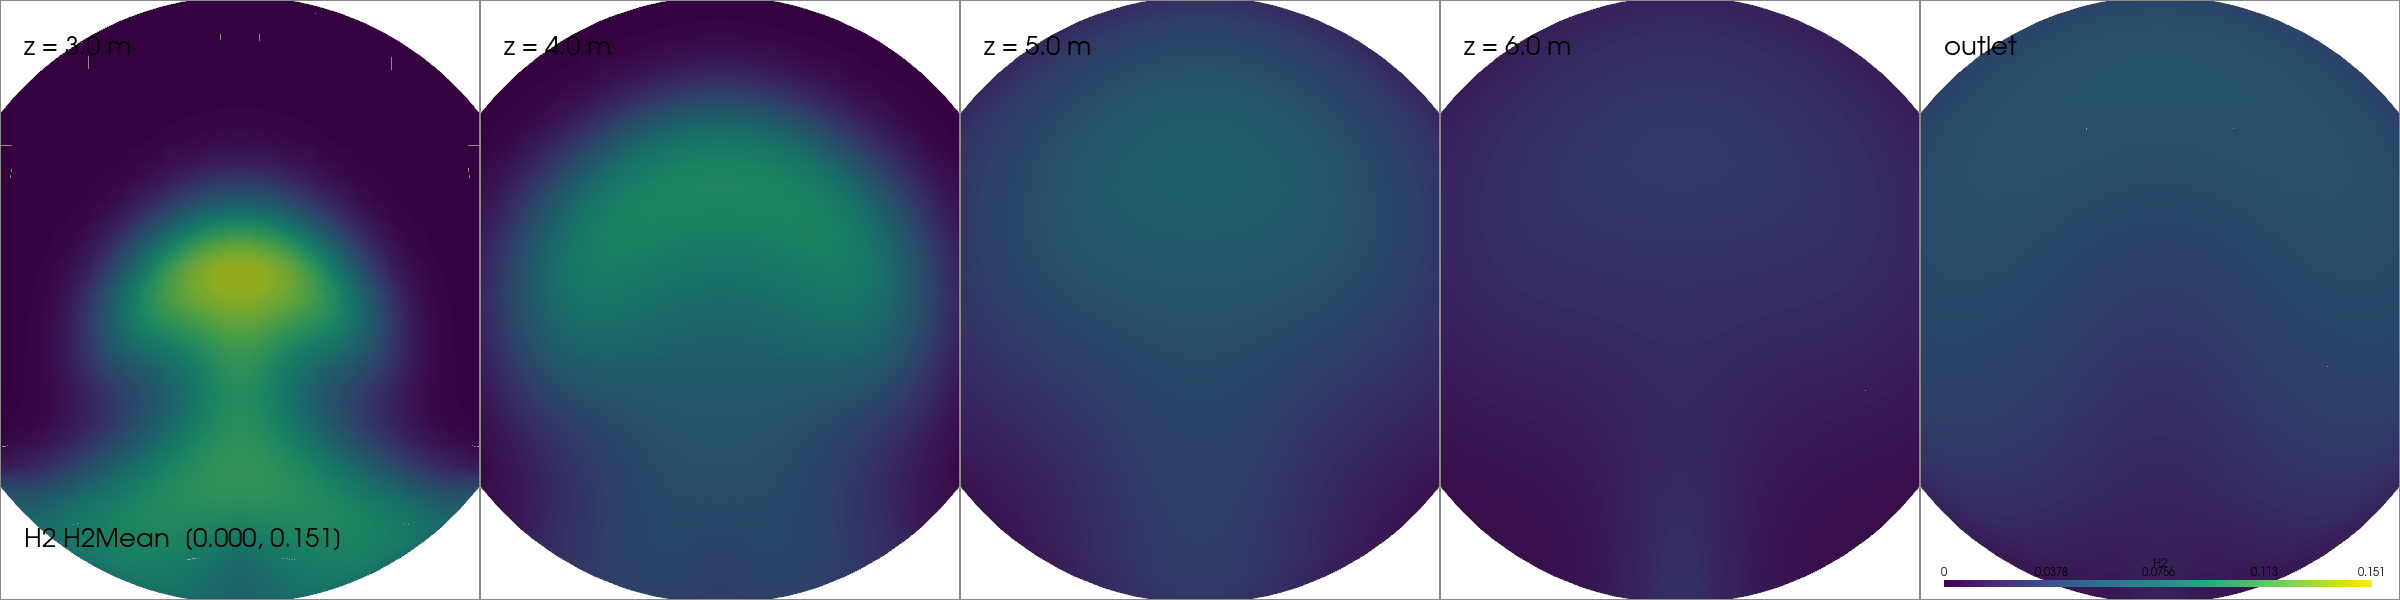
\includegraphics[width=\textwidth]{../doe/results_full_90deg_bottom/case_04/figures/fig_H2_strip.png}
        \caption{Bottom injection (\(\CoV = 0.271\)). At \(z=3\,\mathrm{m}\)
        the plume is a concentrated mushroom in the lower half; even at the
        outlet the concentration gradient persists.}
        \label{fig:strip_04_bot}
    \end{subfigure}
    \caption{Cross-sectional H\(_2\) strip for case~04
    (\(\dD=0.252\), \(\VR=3.81\)) at \(90^\circ\).
    Top injection (a) vs.\ bottom injection (b).
    Both images are time-averaged (\texttt{H2Mean}) at
    \(t=\SI{1.2}{\second}\).}
    \label{fig:bot_strip_04}
\end{figure}

With top injection (Fig.~\ref{fig:strip_04_top}), the high-\VR{}
jet punches downward through the pipe diameter. Buoyancy then
\emph{prevents} the lighter \Hi{} from falling further, so the gas
flattens against the upper wall and spreads laterally into a thin,
wide layer with maximum surface area for turbulent diffusion. By
\(z \approx 5\,D\) the cross-section is virtually uniform
(\(\CoV = 0.066\)).

With bottom injection (Fig.~\ref{fig:strip_04_bot}), the same jet
punches upward. Buoyancy now \emph{assists} the jet: the plume
rises as a coherent, narrow column that never fans out laterally.
By the outlet the \Hi{} is concentrated in the upper half as a
mushroom-shaped streak rather than spread across the full pipe
(\(\CoV = 0.271\), a factor of four worse).

Figure~\ref{fig:bot_strip_08} shows the same comparison at low
\VR{} (case~08, \(\VR = 0.69\)), where neither configuration
mixes well but the physics diverge even further.

\begin{figure}[H]
    \centering
    \begin{subfigure}[b]{\textwidth}
        \centering
        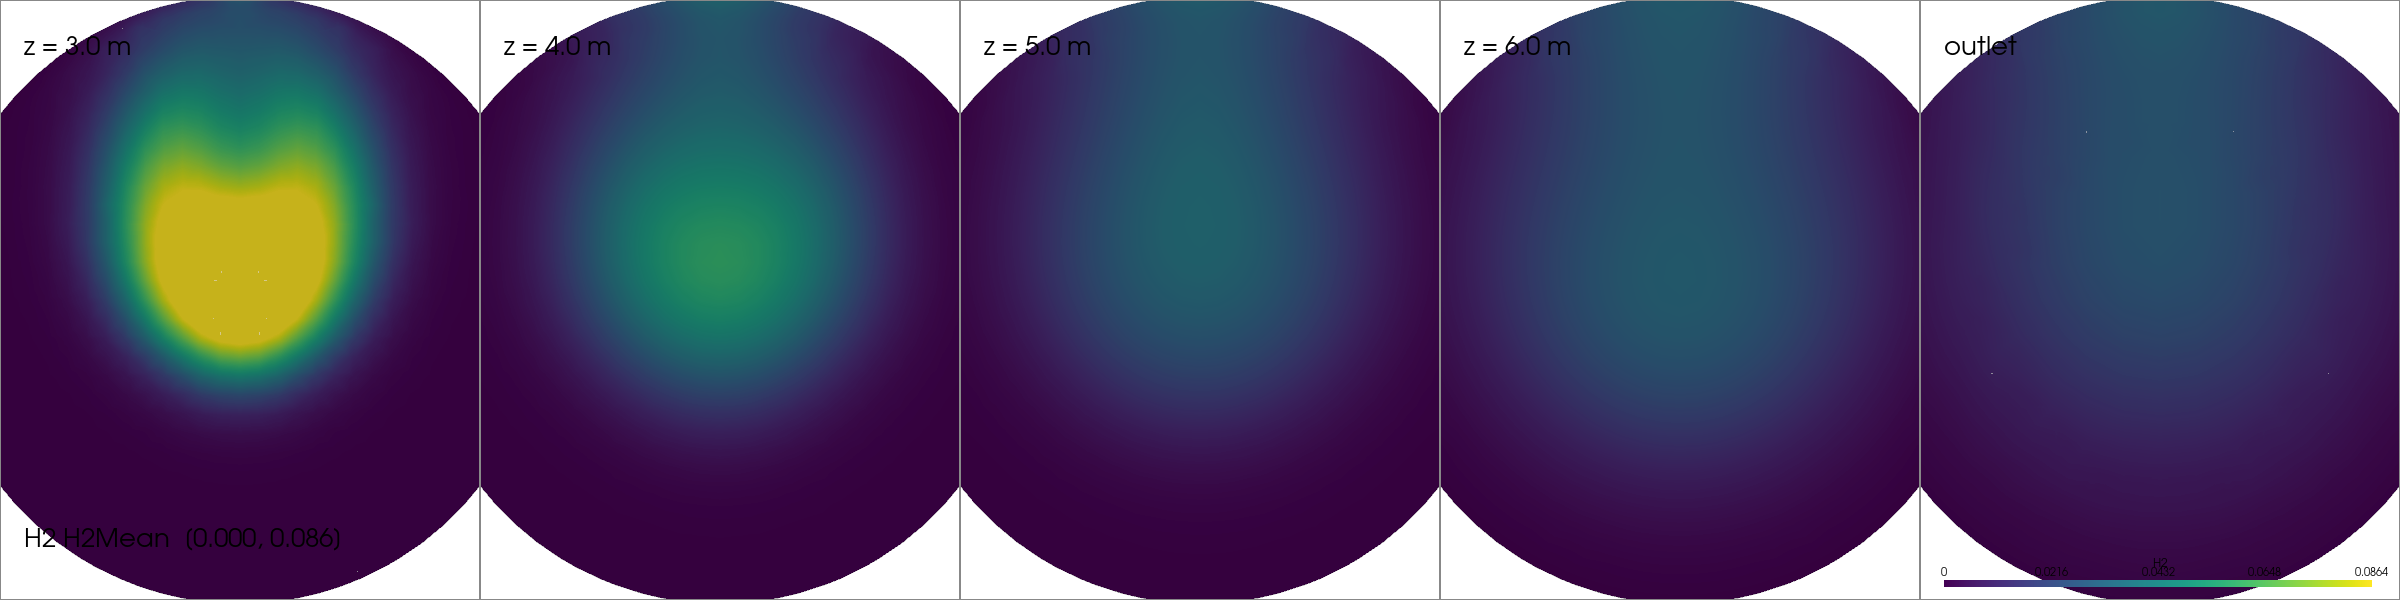
\includegraphics[width=\textwidth]{../doe/results_full/cases/case_08/figures/fig_H2_strip.png}
        \caption{Top injection (\(\CoV = 0.707\)). The low-momentum jet
        barely penetrates, but spreads at the crown.}
        \label{fig:strip_08_top}
    \end{subfigure}\\[6pt]
    \begin{subfigure}[b]{\textwidth}
        \centering
        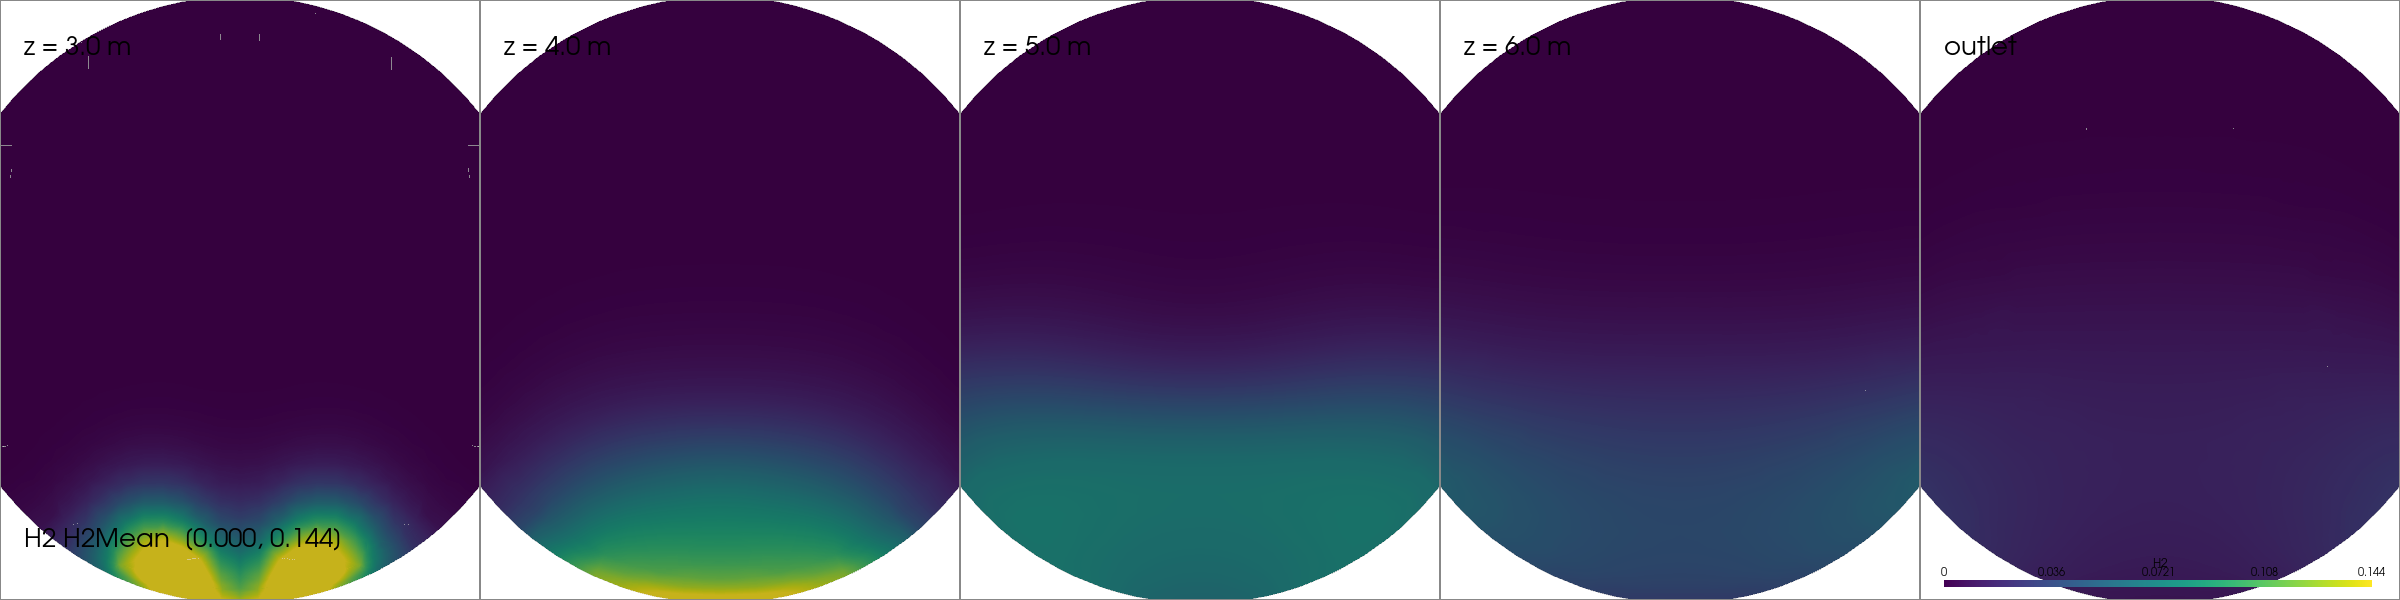
\includegraphics[width=\textwidth]{../doe/results_full_90deg_bottom/case_08/figures/fig_H2_strip.png}
        \caption{Bottom injection (\(\CoV = 0.911\)). The plume stratifies
        into a horizontal layer at the bottom of the pipe; by the outlet a
        clear two-layer structure is visible.}
        \label{fig:strip_08_bot}
    \end{subfigure}
    \caption{Cross-sectional H\(_2\) strip for case~08
    (\(\dD=0.382\), \(\VR=0.69\)) at \(90^\circ\).
    At low \VR{} the buoyancy effect dominates: the bottom-injection
    plume stratifies rather than spreading.}
    \label{fig:bot_strip_08}
\end{figure}

\subsection{Longitudinal centreline comparison}
\label{sec:bot_long}

Figure~\ref{fig:bot_long_04} shows the centreline slice for the
same case~04 pair. With top injection the plume penetrates deep into
the pipe and then diffuses uniformly downstream; with bottom
injection the plume clings to the bottom wall and rises slowly ---
the bright yellow concentration core extends several diameters
further downstream before decaying.

\begin{figure}[H]
    \centering
    \begin{subfigure}[b]{\textwidth}
        \centering
        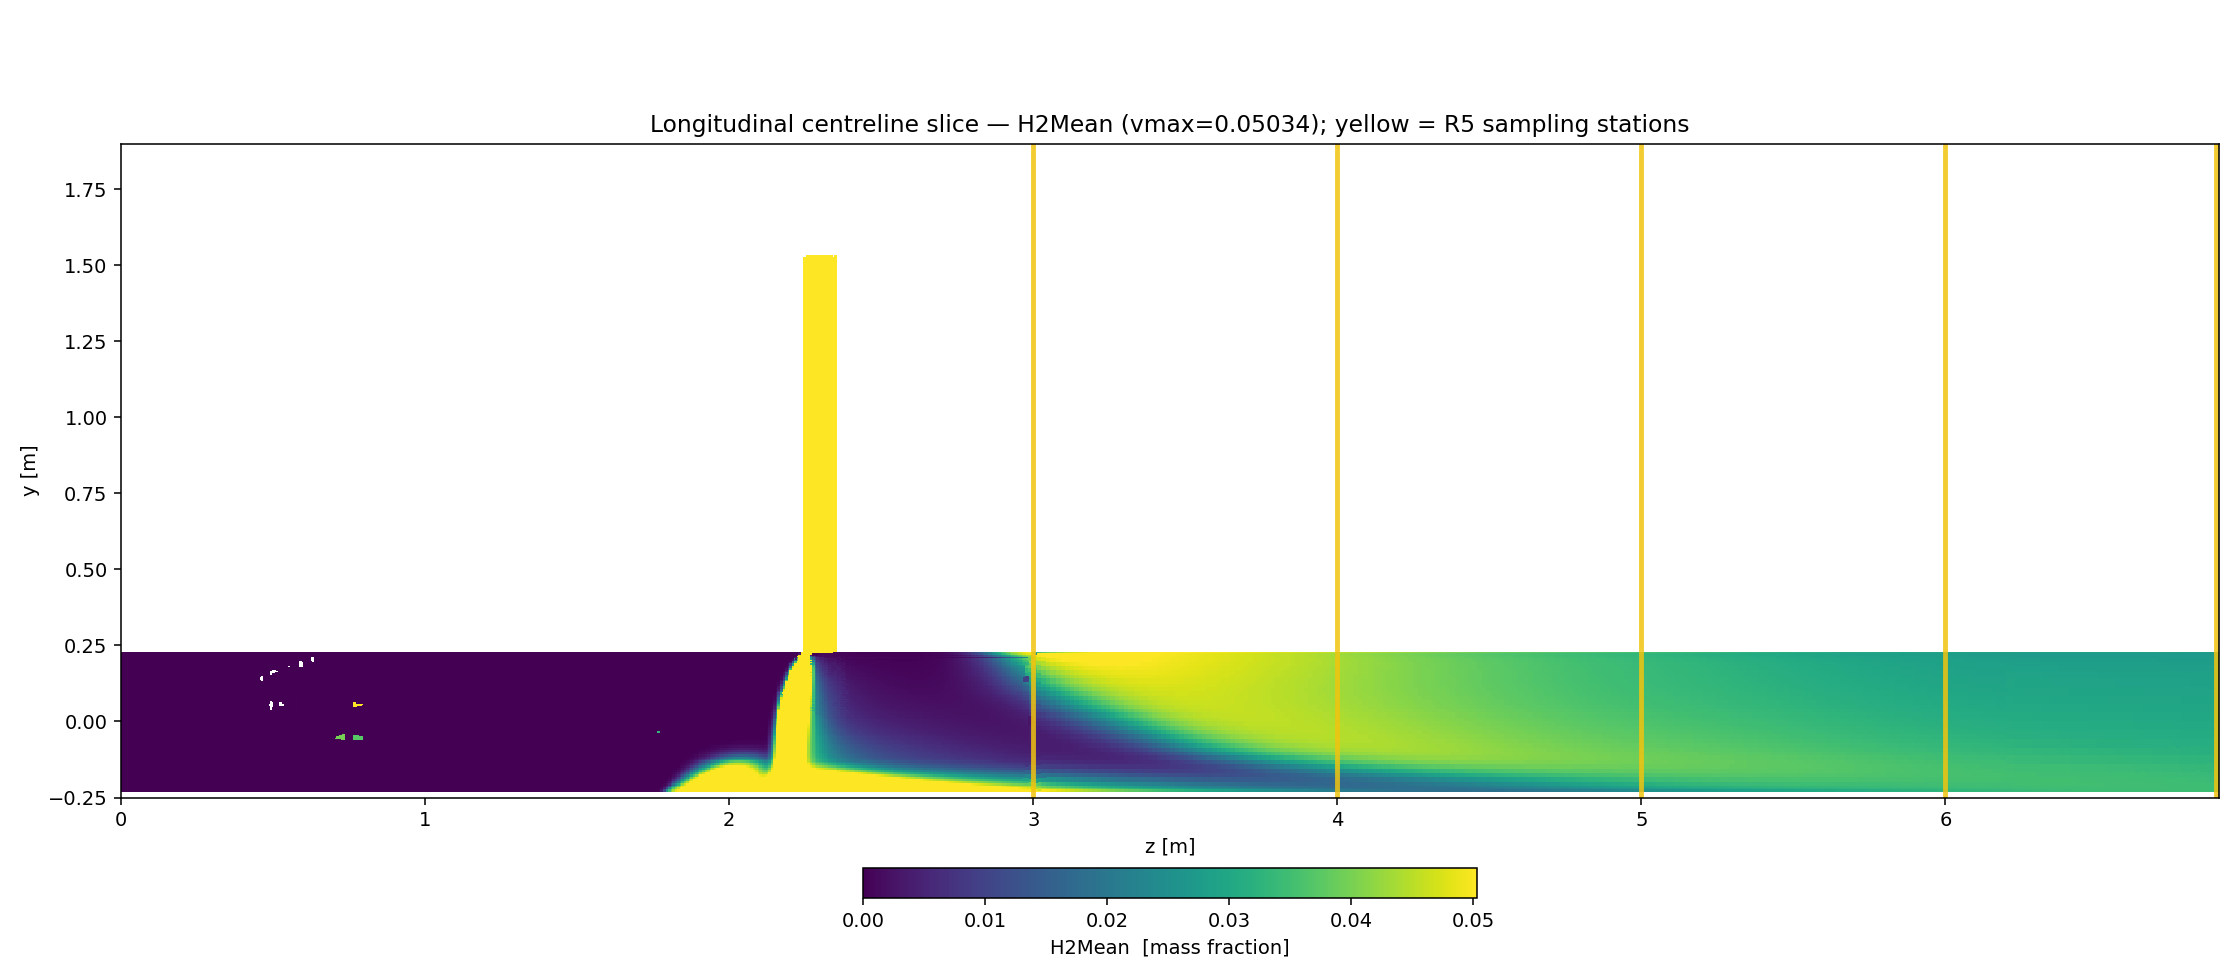
\includegraphics[width=\textwidth]{../doe/results_full/cases/case_04/figures/fig_H2_long.png}
        \caption{Top injection --- the jet impinges downward; \Hi{}
        fills the pipe cross-section by \(z\approx 3\,\mathrm{m}\).}
    \end{subfigure}\\[4pt]
    \begin{subfigure}[b]{\textwidth}
        \centering
        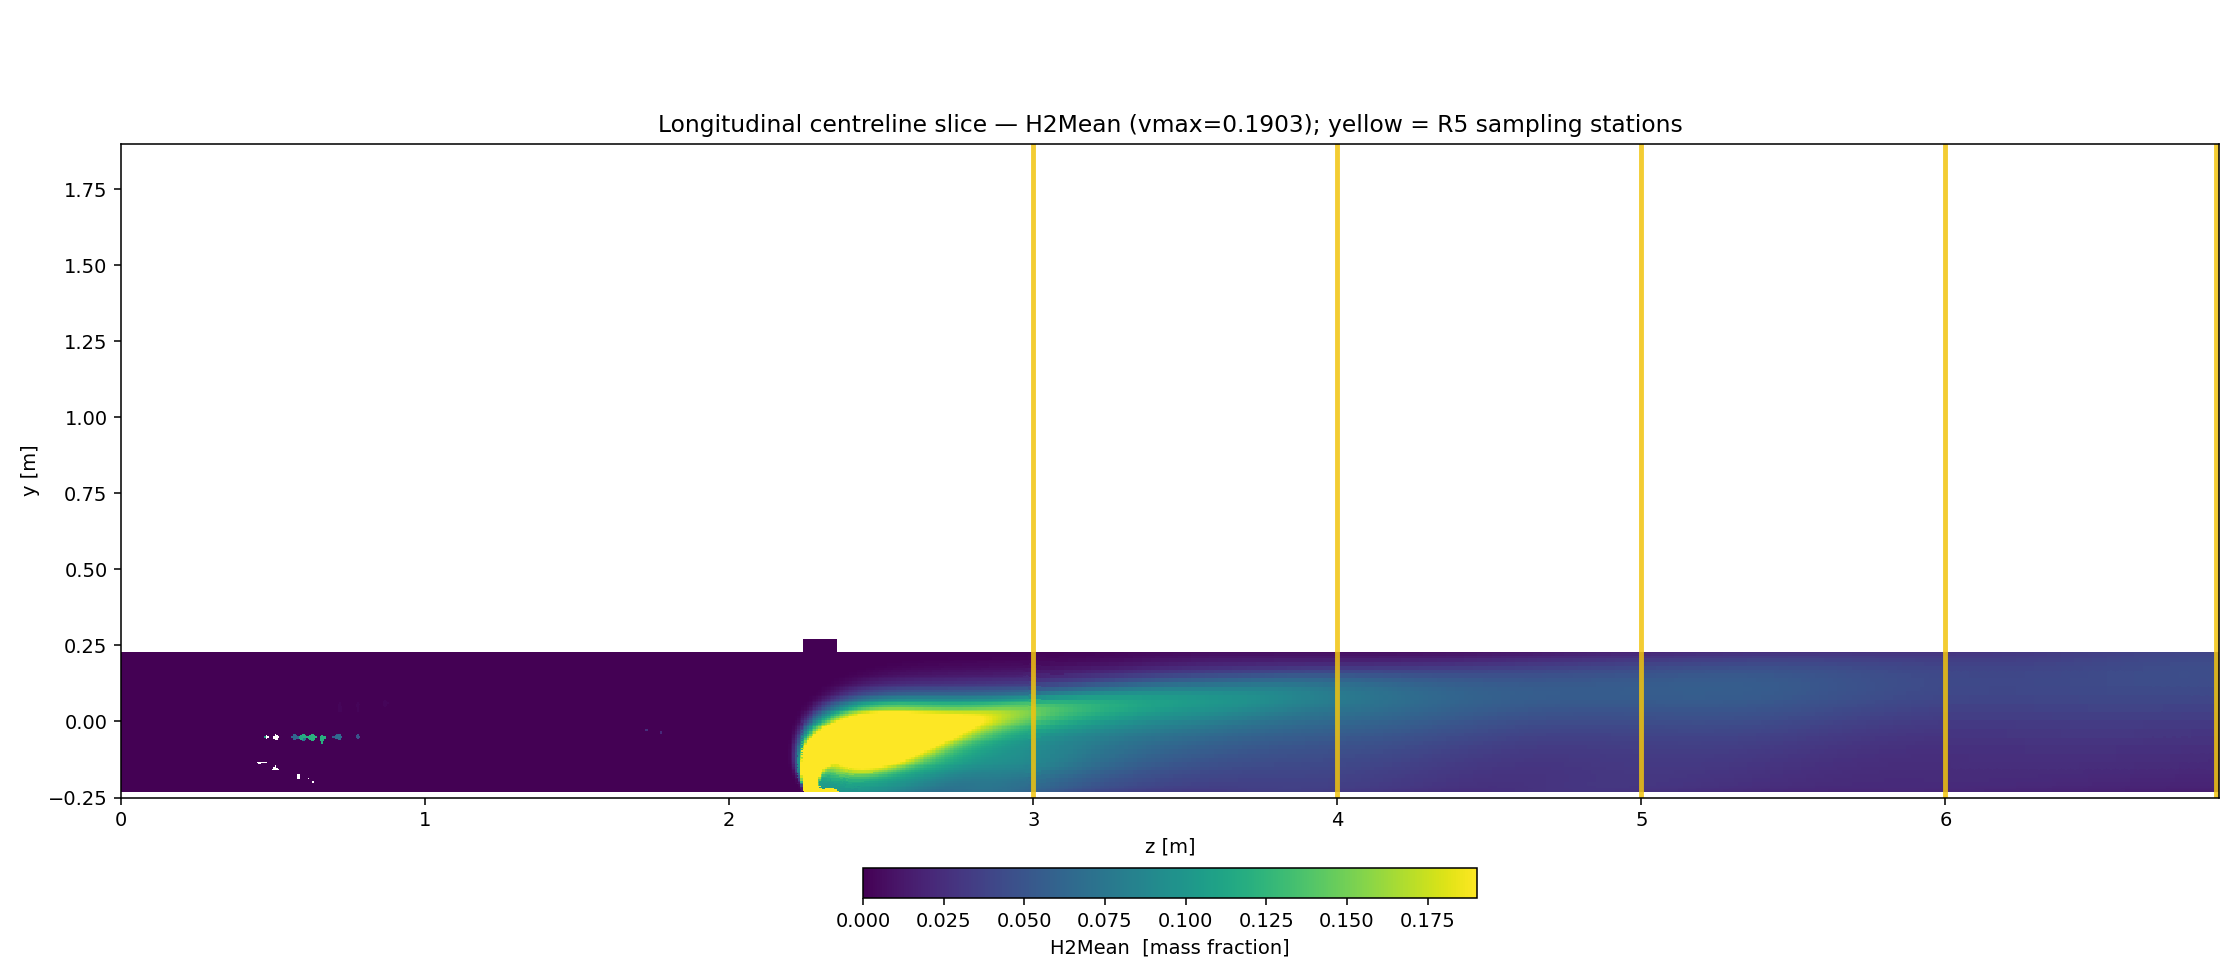
\includegraphics[width=\textwidth]{../doe/results_full_90deg_bottom/case_04/figures/fig_H2_long.png}
        \caption{Bottom injection --- the plume hugs the bottom wall
        and rises as a narrow column. Peak mass fraction is
        \(0.19\) vs.\ \(0.05\) for top injection.}
    \end{subfigure}
    \caption{Longitudinal centreline slice of
    \(Y_{\Hi}\) (\texttt{H2Mean}) for case~04 at \(90^\circ\).}
    \label{fig:bot_long_04}
\end{figure}

\noindent Figure~\ref{fig:cov_zD_topbot} compares the \CoV{} decay
along the pipe for the same case~04 pair.  With top injection
\CoV{} decays steeply (reaching \(\sim\!0.07\) at the outlet);
with bottom injection the decay is much slower, levelling off near
\(\CoV \sim 0.28\) as the coherent rising plume fails to spread
laterally.

\begin{figure}[H]
    \centering
    \begin{minipage}[t]{0.48\textwidth}
       \centering
       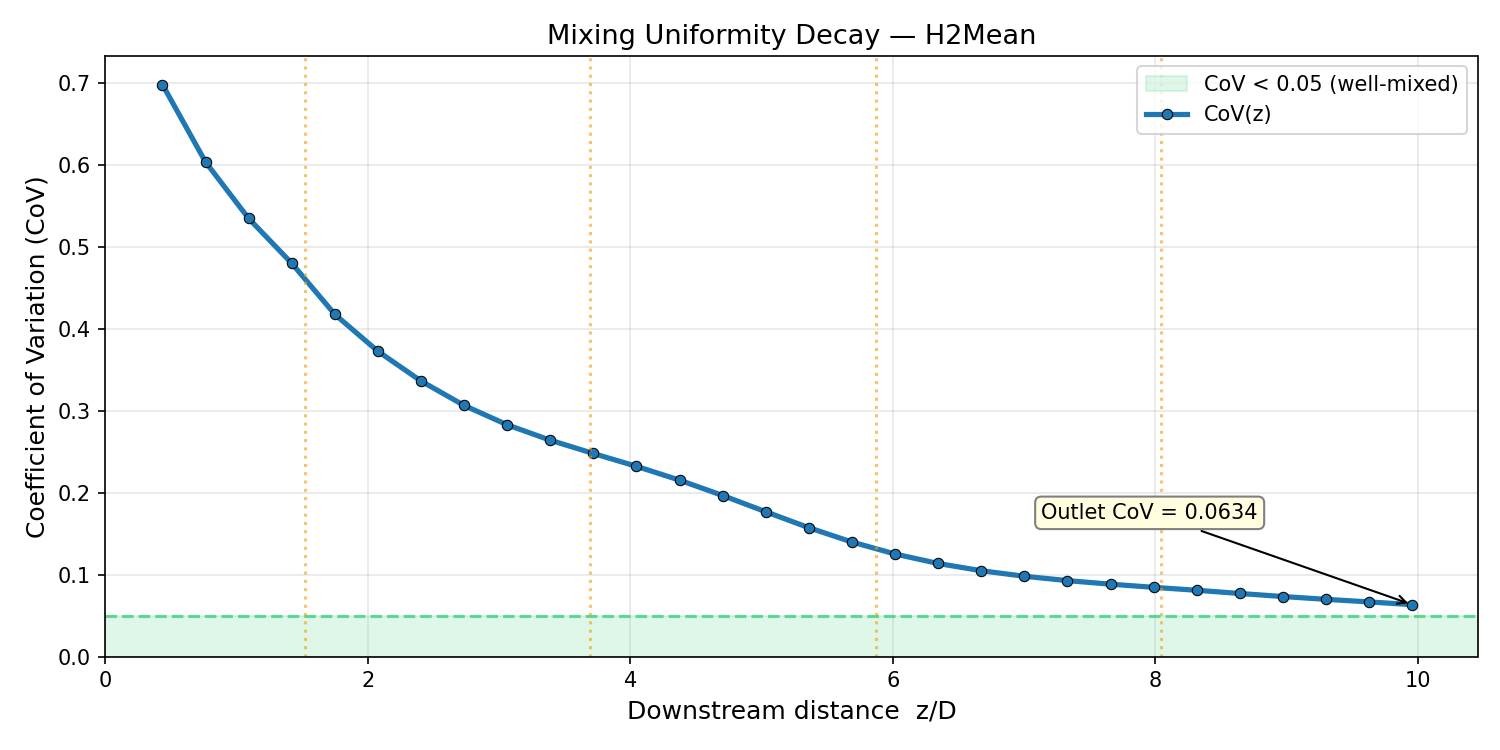
\includegraphics[width=\textwidth]{../doe/results_full/cases/case_04/figures/fig_CoV_vs_zD.png}
    \end{minipage}\hfill
    \begin{minipage}[t]{0.48\textwidth}
       \centering
       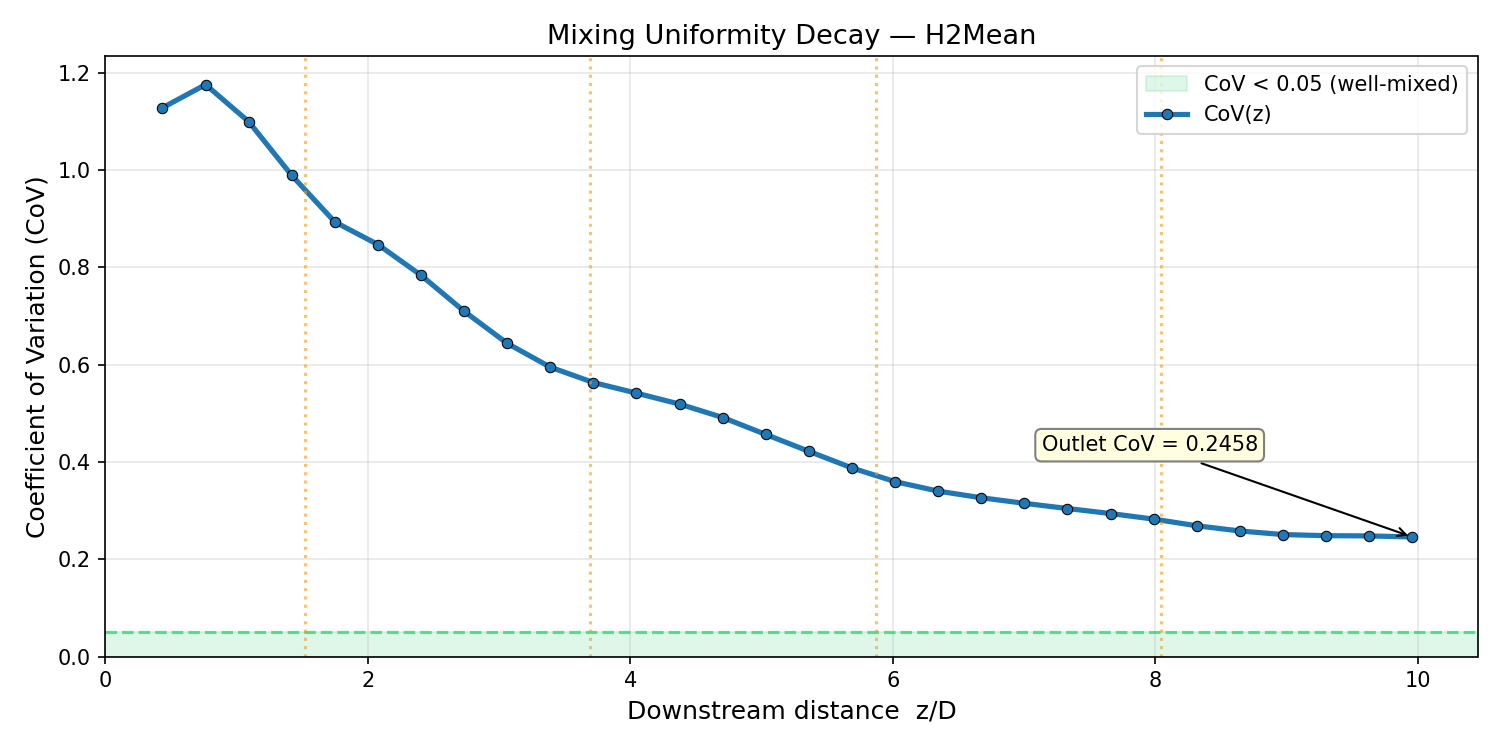
\includegraphics[width=\textwidth]{../doe/results_full_90deg_bottom/case_04/figures/fig_CoV_vs_zD.png}
    \end{minipage}
    \caption{\CoV{} vs.\ downstream distance \(z/D\) for case~04
    (\(\VR=3.81\)) at \(90^\circ\): top injection (left) vs.\
    bottom injection (right).  Top injection reaches near the
    \(\CoV = 0.05\) threshold; bottom injection plateaus at
    \(\sim\!5\times\) higher \CoV.  Green band =
    \(\CoV < 0.05\).}
    \label{fig:cov_zD_topbot}
\end{figure}

% =====================================================================
%  9. FOUR-CAMPAIGN CROSS-CAMPAIGN SYNTHESIS
% =====================================================================
\section{Cross-campaign synthesis: injection side effect}
\label{sec:cross_side}

With all four campaigns completed --- \(90^\circ\) top (8~cases),
\(30^\circ\) top (9~cases), \(90^\circ\) bottom (13~cases) and
\(30^\circ\) bottom (10~cases) --- a full factorial comparison of
angle~\(\times\)~side is possible. All 40 valid cases use the same
LP-filtered \(|\Delta p|\) methodology
(Section~\ref{sec:dp_filter}) and the same area-weighted
\CoV{} from the outlet snapshot.

\subsection{CoV vs VR: universal power-law scaling}
\label{sec:cross4_vr}

Figure~\ref{fig:cross4_cov_vr} extends the two-campaign power-law
plot of Section~\ref{sec:cross_scaling} to all four campaigns. The
fits are:
\begin{align}
90^\circ\;\text{top}:&\quad \CoV \approx 0.47\,\VR^{-1.16},
& R^2 = 0.80, \label{eq:fit_90t}\\
30^\circ\;\text{top}:&\quad \CoV \approx 0.33\,\VR^{-1.88},
& R^2 = 0.80, \label{eq:fit_30t}\\
90^\circ\;\text{bot}:&\quad \CoV \approx 0.89\,\VR^{-0.91},
& R^2 = 0.90, \label{eq:fit_90b}\\
30^\circ\;\text{bot}:&\quad \CoV \approx 1.13\,\VR^{-0.72},
& R^2 = 0.72. \label{eq:fit_30b}
\end{align}
Two patterns emerge. First, the top-injection exponents
(\(-1.16\), \(-1.88\)) are steeper than their bottom-injection
counterparts (\(-0.91\), \(-0.72\)): increasing \VR{} buys
proportionally more mixing from the top. Second, the intercepts
(\(A\)) are higher for bottom injection (\(0.89\), \(1.13\)) than
for top (\(0.47\), \(0.33\)), so even the extrapolated low-\VR{}
behaviour is worse for bottom injection.

\begin{figure}[H]
    \centering
    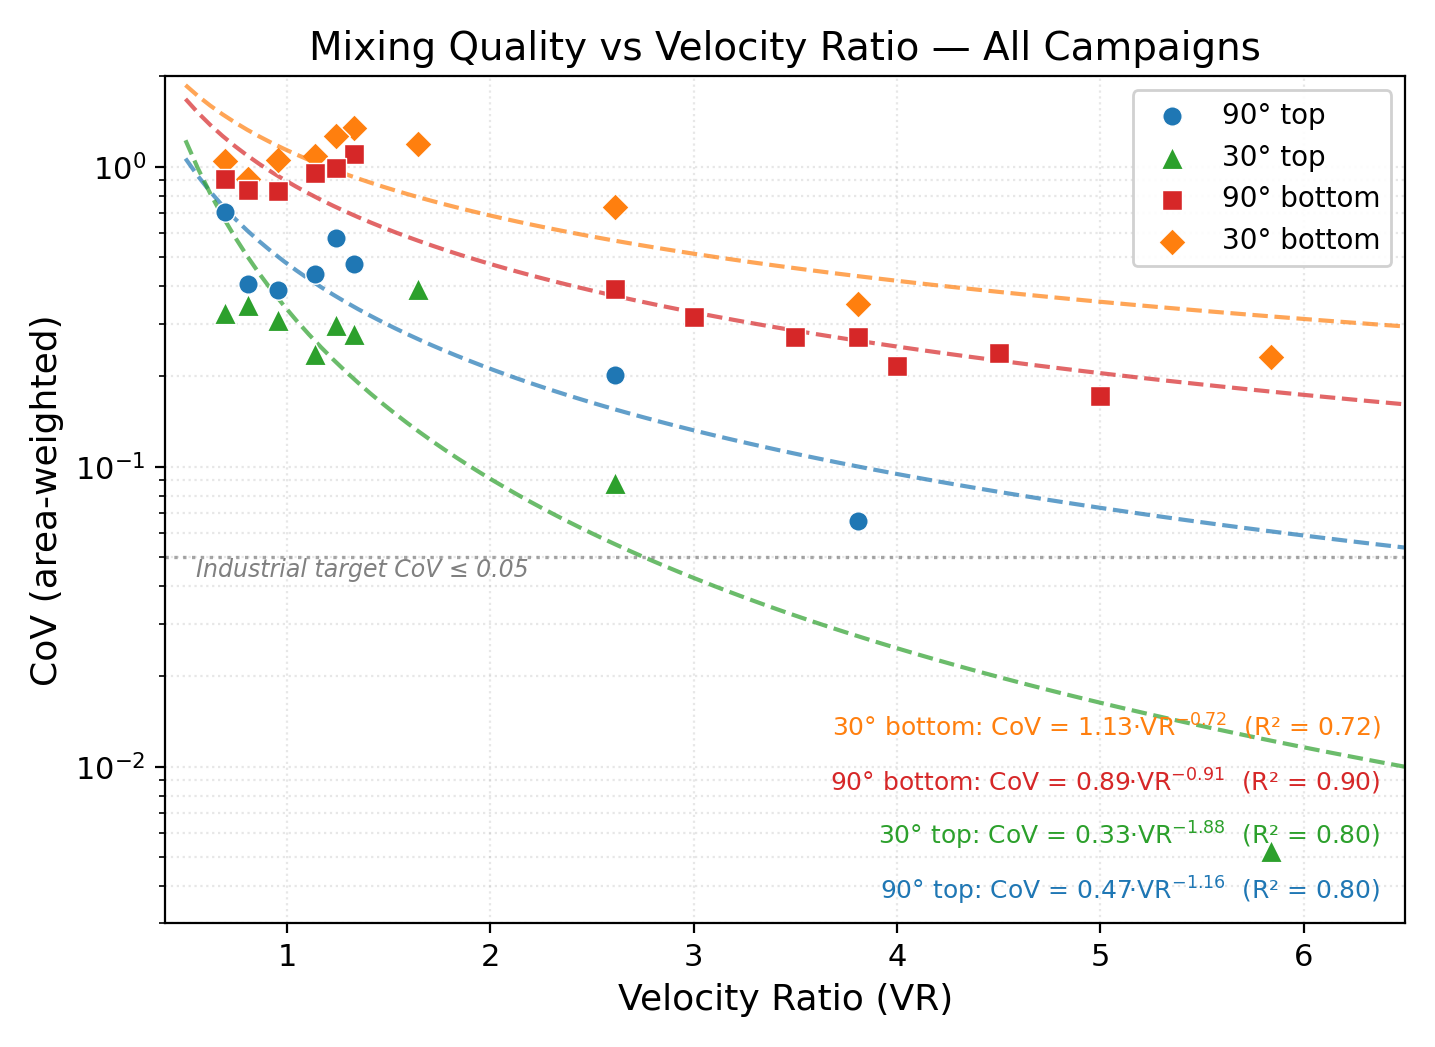
\includegraphics[width=0.9\textwidth]{../doe/cross_campaign/figures/fig1_CoV_vs_VR.png}
    \caption{Power-law fit of \CoV{} vs.\ \VR{} for all four
    campaigns. The \(30^\circ\) top campaign has the steepest slope;
    the \(30^\circ\) bottom campaign has the shallowest. The dashed
    grey line marks the industrial \(\CoV \le 0.05\) target.}
    \label{fig:cross4_cov_vr}
\end{figure}

\subsection{Matched-pair comparison: top vs bottom}
\label{sec:cross4_pairs}

Figure~\ref{fig:cross4_matched} uses the same matched-pair
methodology as Section~\ref{sec:cross_pairs}, but now compares
\emph{top vs.\ bottom} at fixed \((\dD,\VR)\). Eight matched pairs
exist at \(90^\circ\) and nine at \(30^\circ\). In \textbf{every
single pair} (17 out of 17), the top-injection case achieves a
lower \CoV{} than the corresponding bottom-injection case. The
median \CoV{} degradation from top to bottom is \(+109\,\%\)
at \(90^\circ\) and \(+324\,\%\) at \(30^\circ\).

Under the null hypothesis that injection side has no effect, the
probability of all 17 pairs having the same sign is
\(2^{1-17} = 1.5\times 10^{-5}\), so the finding is highly
statistically significant regardless of per-pair magnitude.

\begin{figure}[H]
    \centering
    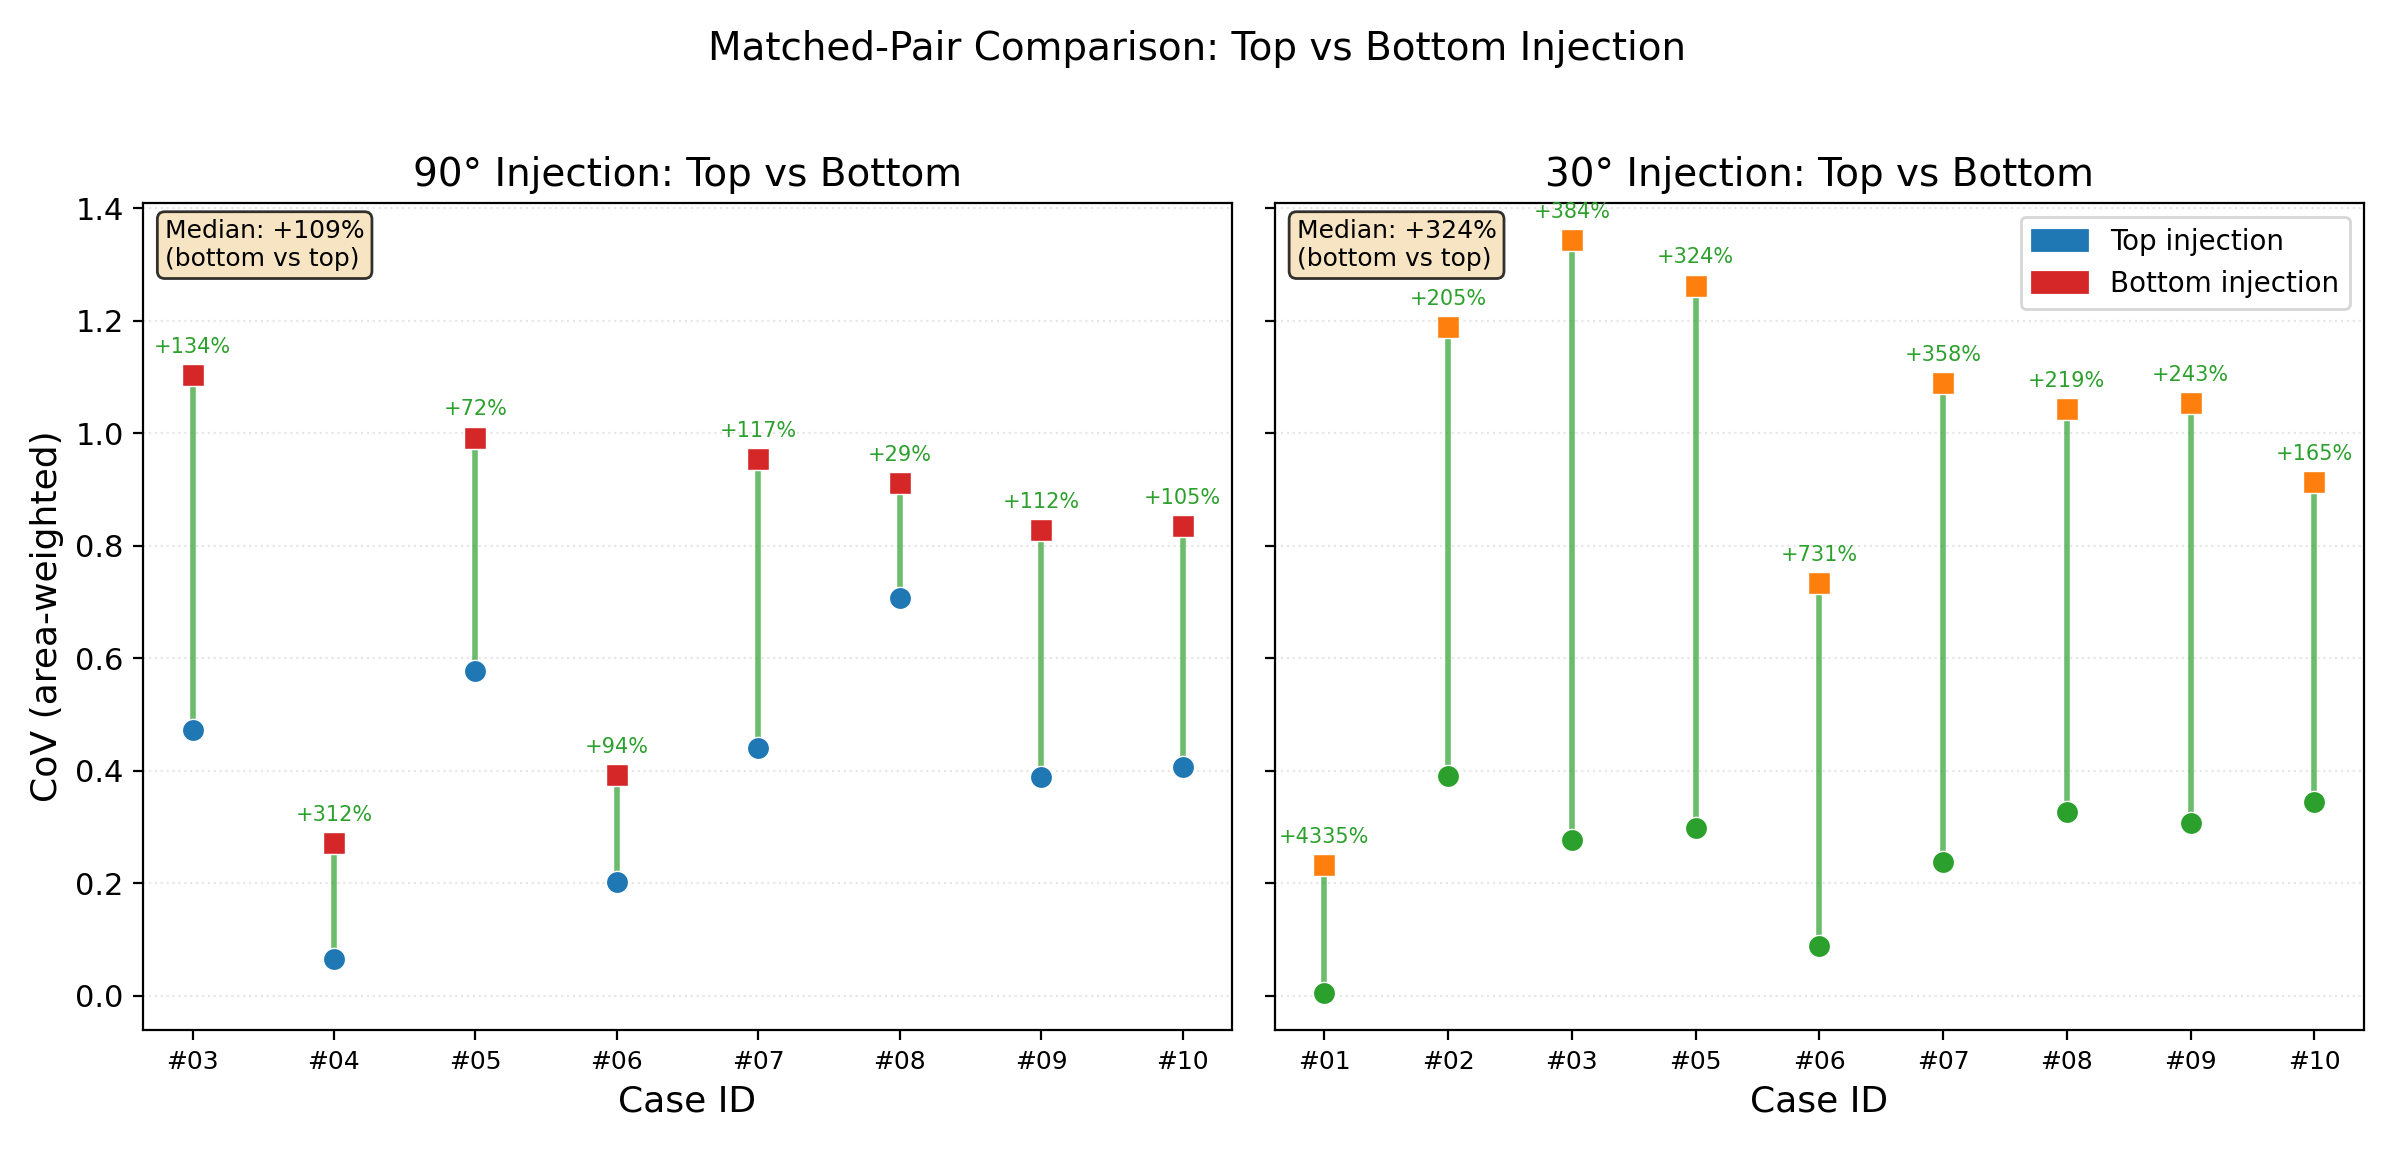
\includegraphics[width=\textwidth]{../doe/cross_campaign/figures/fig2_matched_pairs_top_vs_bottom.png}
    \caption{Matched-pair arrow plot, top vs.\ bottom injection.
    Left: \(90^\circ\); right: \(30^\circ\). Green arrows indicate
    that bottom injection has a higher (worse) \CoV. Every arrow is
    green: top injection is strictly better at every matched
    operating point. Percentage labels show the per-case \CoV{}
    increase going from top to bottom.}
    \label{fig:cross4_matched}
\end{figure}

\subsection{Pressure-drop trends across all four campaigns}
\label{sec:cross4_dp}

Unlike the mixing metric \CoV, the LP-filtered pressure drop
\(|\Delta p_{\mathrm{rgh}}|\) carries a large acoustic uncertainty.
The compressible solver (\texttt{rhoReactingBuoyantFoam}) captures
high-frequency pressure waves whose standard deviation after LP
filtering is \(\sigma \approx 10\)-\(\SI{23}{\kilo\pascal}\),
while the LP-filtered \emph{mean} \(|\Delta p|\) is only
\(0\)-\(\SI{8}{\kilo\pascal}\) (signal-to-noise ratio typically
\(\sim 0.05\)-\(0.19\)). The analysis below should therefore be
read as trend-level; case-to-case precision is
\(\pm\SI{0.5}{\kilo\pascal}\) at best.

\subsubsection{Injection side does not affect pressure drop}

Figure~\ref{fig:cross4_bar_dP} shows the median
\(|\Delta p_{\mathrm{rgh}}|\) by campaign. The four medians are
\SI{1.05}{\kilo\pascal} (\(90^\circ\)~top),
\SI{0.53}{\kilo\pascal} (\(30^\circ\)~top),
\SI{1.58}{\kilo\pascal} (\(90^\circ\)~bot) and
\SI{1.02}{\kilo\pascal} (\(30^\circ\)~bot) --- all within a
\(\sim\SI{1}{\kilo\pascal}\) band. Switching from top to bottom
injection therefore does \emph{not} save pumping energy; it only
degrades mixing. Top injection is strictly dominant in the present
parameter space.

\begin{figure}[H]
    \centering
    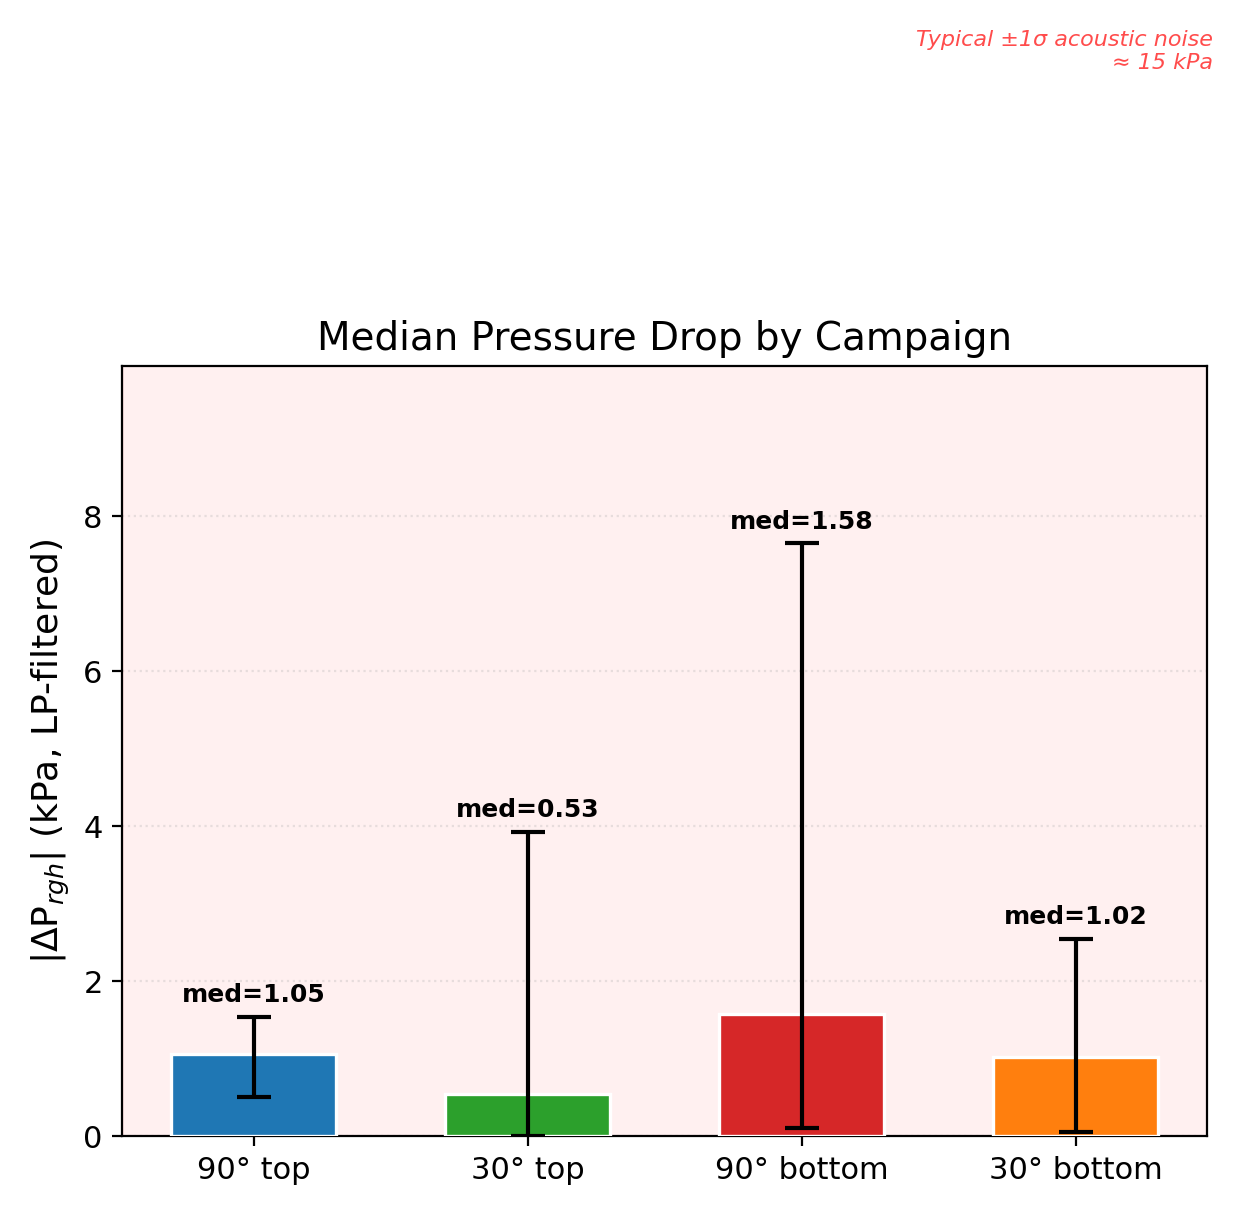
\includegraphics[width=0.75\textwidth]{../doe/cross_campaign/figures/fig11_bar_median_dP.png}
    \caption{Median \(|\Delta p_{\mathrm{rgh}}|\) by campaign with
    min--max error bars. The light-red band indicates the typical
    \(\pm 1\sigma\) acoustic noise (\(\approx\SI{15}{\kilo\pascal}\)),
    confirming that all four medians are small relative to the
    acoustic floor. The inter-campaign differences are within the
    noise band and therefore not statistically significant.}
    \label{fig:cross4_bar_dP}
\end{figure}

\textbf{Physical justification.} The junction pressure loss is set
by the local momentum budget at the T-junction: the abrupt area
expansion and the turning of the branch flow into the main pipe.
These are determined by the branch-to-main area ratio \((\dD)^2\)
and the geometric turning angle \(\alpha\), both of which are
\emph{identical} for top and bottom injection. Flipping the branch
from top to bottom changes the direction of the buoyancy force on
the \emph{downstream} plume but does not alter the junction
geometry, so the junction loss coefficient
\(K = |\Delta p|/q_{\mathrm{dyn,main}}\) is unchanged.

\subsubsection{The \texorpdfstring{$30^\circ$}{30 deg} tilt reduces pressure drop}

Comparing the two angles at the same injection side:
\(30^\circ\)~top (\SI{0.53}{\kilo\pascal}) is roughly half of
\(90^\circ\)~top (\SI{1.05}{\kilo\pascal}); \(30^\circ\)~bot
(\SI{1.02}{\kilo\pascal}) is below \(90^\circ\)~bot
(\SI{1.58}{\kilo\pascal}). This is consistent with the
matched-pair finding in Section~\ref{sec:cross_pairs} and with
the classical handbook result of
\citet{idelchik1986handbook}: the junction loss coefficient for a
diverging tee decreases monotonically as the branch angle
decreases from \(90^\circ\) toward \(0^\circ\) (co-flow), because
the branch jet at \(30^\circ\) enters with a large streamwise
momentum component and only needs to turn through \(30^\circ\)
instead of \(90^\circ\). The \(60^\circ\) of saved turning loss is
never generated.

\subsubsection{\texorpdfstring{$|\Delta p|$}{|dP|} vs velocity ratio}

Figure~\ref{fig:cross4_dP_vr} plots the LP-filtered
\(\Delta p_{\mathrm{rgh}}\) against \VR{} with \(\pm 1\sigma\)
acoustic error bars.

\begin{figure}[H]
    \centering
    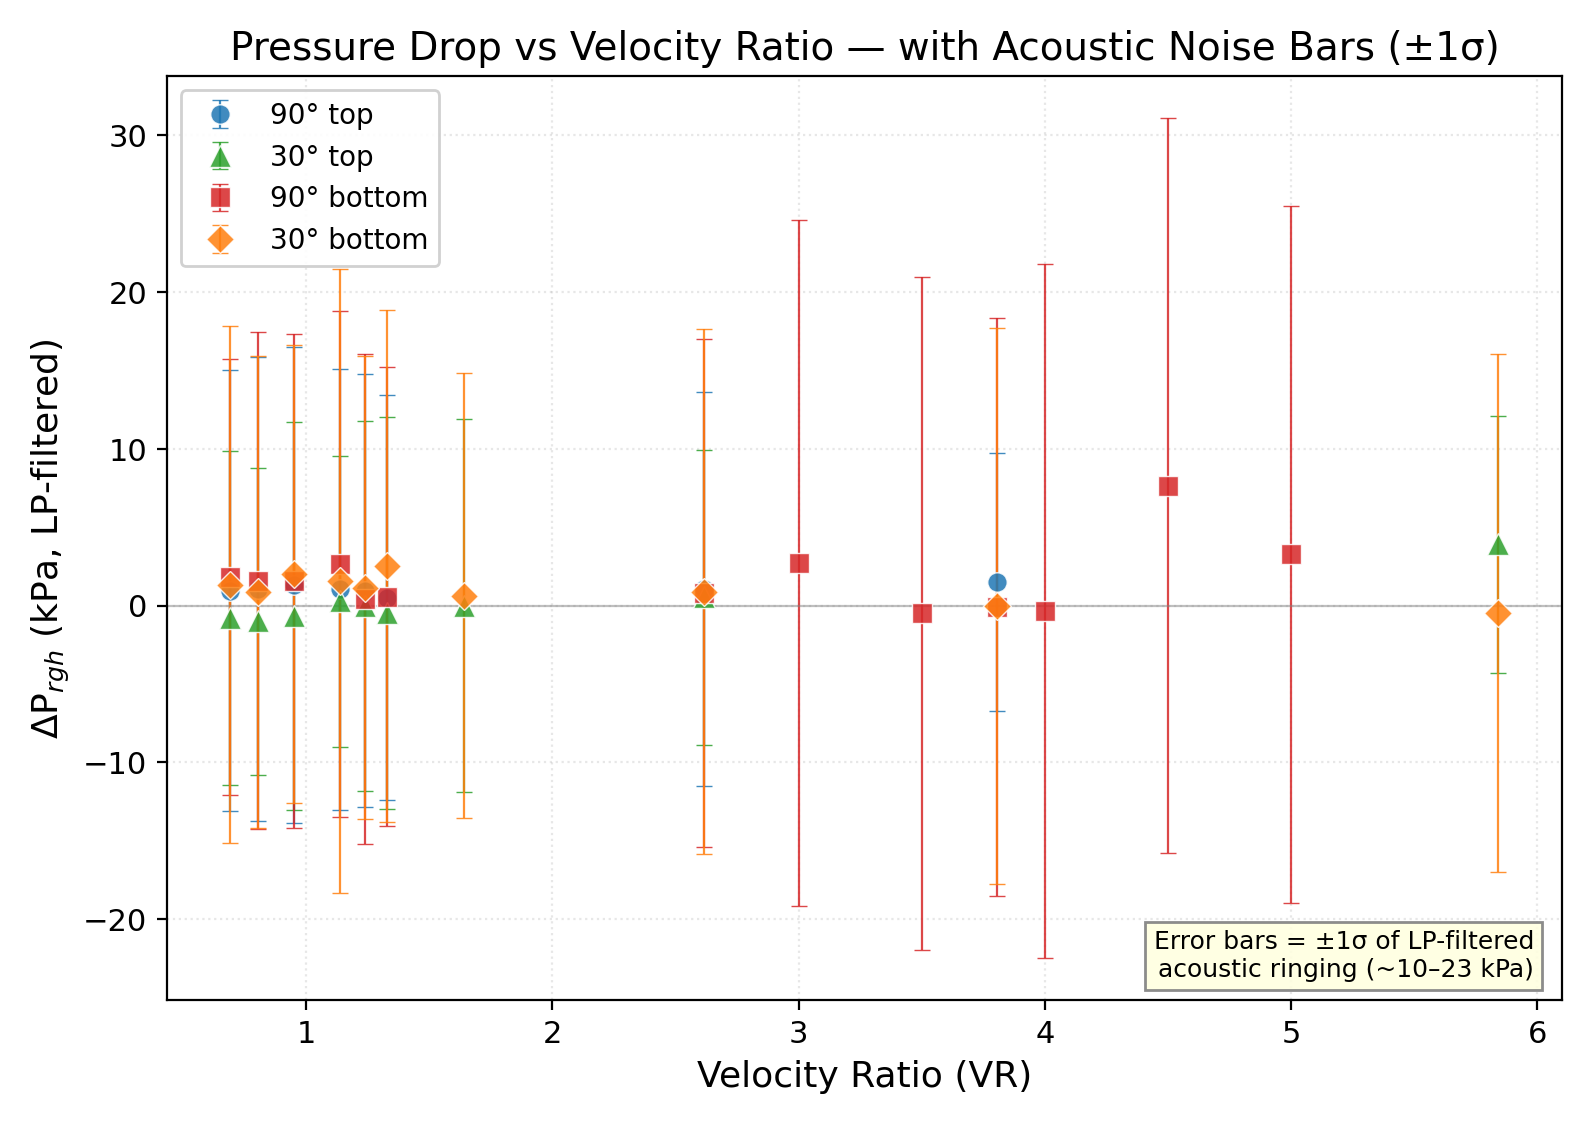
\includegraphics[width=0.95\textwidth]{../doe/cross_campaign/figures/fig8_dP_vs_VR_errorbars.png}
    \caption{LP-filtered \(\Delta p_{\mathrm{rgh}}\) vs.\ \VR{}
    for all four campaigns. Error bars show \(\pm 1\sigma\) of the
    LP-filtered acoustic ringing (\(\sim 10\)-\(\SI{23}{\kilo\pascal}\)).
    The data points cluster near zero relative to the error bars,
    confirming that pressure drop is a weak signal in the present
    simulation window.}
    \label{fig:cross4_dP_vr}
\end{figure}

Despite the noise, two trends are visible. For
\textbf{top injection} (both angles), \(|\Delta p|\) increases
with \VR{} (\(r = 0.53\) at \(90^\circ\), \(r = 0.98\) at
\(30^\circ\)). This is expected: the junction loss scales as
\(K \cdot q_{\mathrm{branch}} = K \cdot \tfrac{1}{2}\rho
u_{\mathrm{branch}}^{2}\), and since
\(\VR = u_{\mathrm{branch}}/u_{\mathrm{main}}\), higher \VR{}
directly increases the branch dynamic pressure and therefore the
total junction loss. The correlation is stronger at \(30^\circ\)
because the co-flow momentum component grows with \VR{}: at low
\VR{} the tilted jet barely contributes to the streamwise pressure
field, while at high \VR{} it adds significant momentum.

For \textbf{bottom injection}, the correlation breaks down
(\(r = 0.26\) at \(90^\circ\), \(r = -0.78\) at \(30^\circ\)).
The coherent buoyant plume rising from the bottom acts as a
partial obstruction to the main flow, redistributing pressure in
ways that do not scale simply with \VR.

\subsubsection{\texorpdfstring{$|\Delta p|$}{|dP|} vs \texorpdfstring{$d/D$}{d/D}}

Figure~\ref{fig:cross4_dP_dD} shows \(|\Delta p|\) against \(\dD\)
at low \VR{} (\(0.6 \le \VR \le 1.5\)).

\begin{figure}[H]
    \centering
    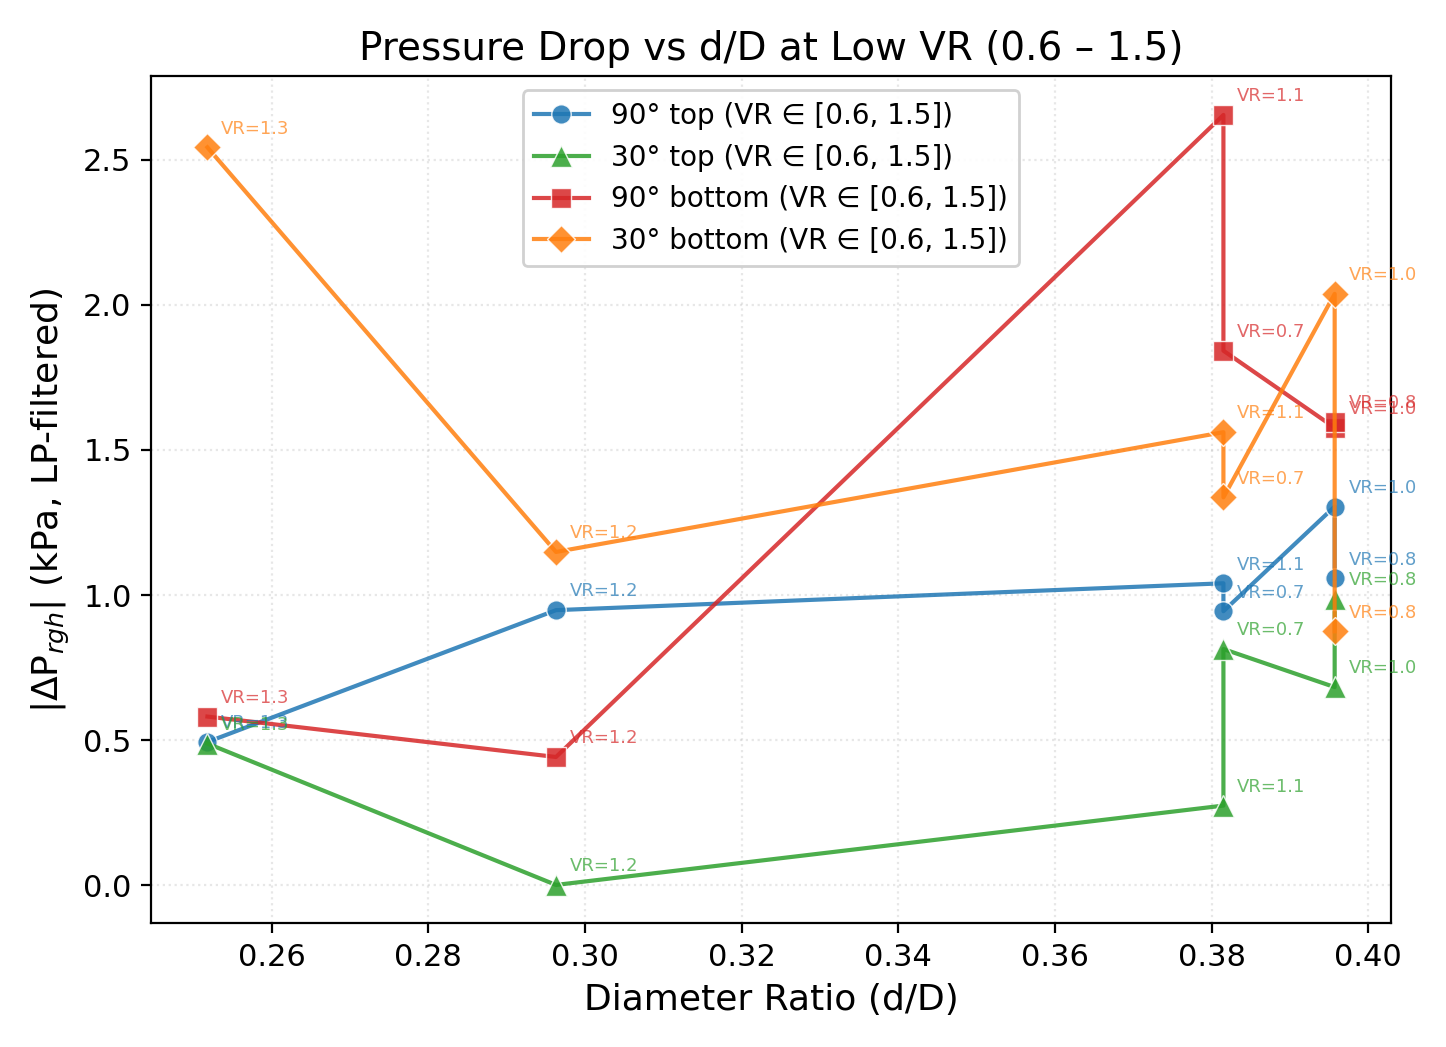
\includegraphics[width=0.85\textwidth]{../doe/cross_campaign/figures/fig10_dP_vs_dD.png}
    \caption{\(|\Delta p_{\mathrm{rgh}}|\) vs.\ \(\dD\) at low
    \VR{} (\(0.6\)-\(1.5\)). At \(90^\circ\) (both top and
    bottom), larger \(\dD\) generally produces higher
    \(|\Delta p|\). At \(30^\circ\), the trend is weaker because
    the co-flow alignment absorbs the additional momentum without
    extra turning loss.}
    \label{fig:cross4_dP_dD}
\end{figure}

At \(90^\circ\), larger \(\dD\) increases \(|\Delta p|\) (from
\(\sim 0.5\,\si{\kilo\pascal}\) at \(\dD = 0.25\) to
\(\sim 1.3\)-\(\SI{2.7}{\kilo\pascal}\) at \(\dD = 0.40\)).
A larger branch port injects more mass (and therefore momentum) at
fixed \VR{}, and at \(90^\circ\) all of this momentum must turn
through a right angle. At \(30^\circ\), the co-flow alignment
absorbs the additional momentum without generating proportional
turning loss, so the \(\dD\) effect on \(|\Delta p|\) is much
weaker.

\subsubsection{Acoustic ringing as a secondary mixing diagnostic}
\label{sec:acoustic_proxy}

An unexpected but physically meaningful finding is that the
\emph{amplitude} of the acoustic ringing (the LP-filter standard
deviation \(\sigma_{|\Delta p|}\)) itself correlates with the
injection configuration
(Fig.~\ref{fig:cross4_acoustic_noise}).

\begin{figure}[H]
    \centering
    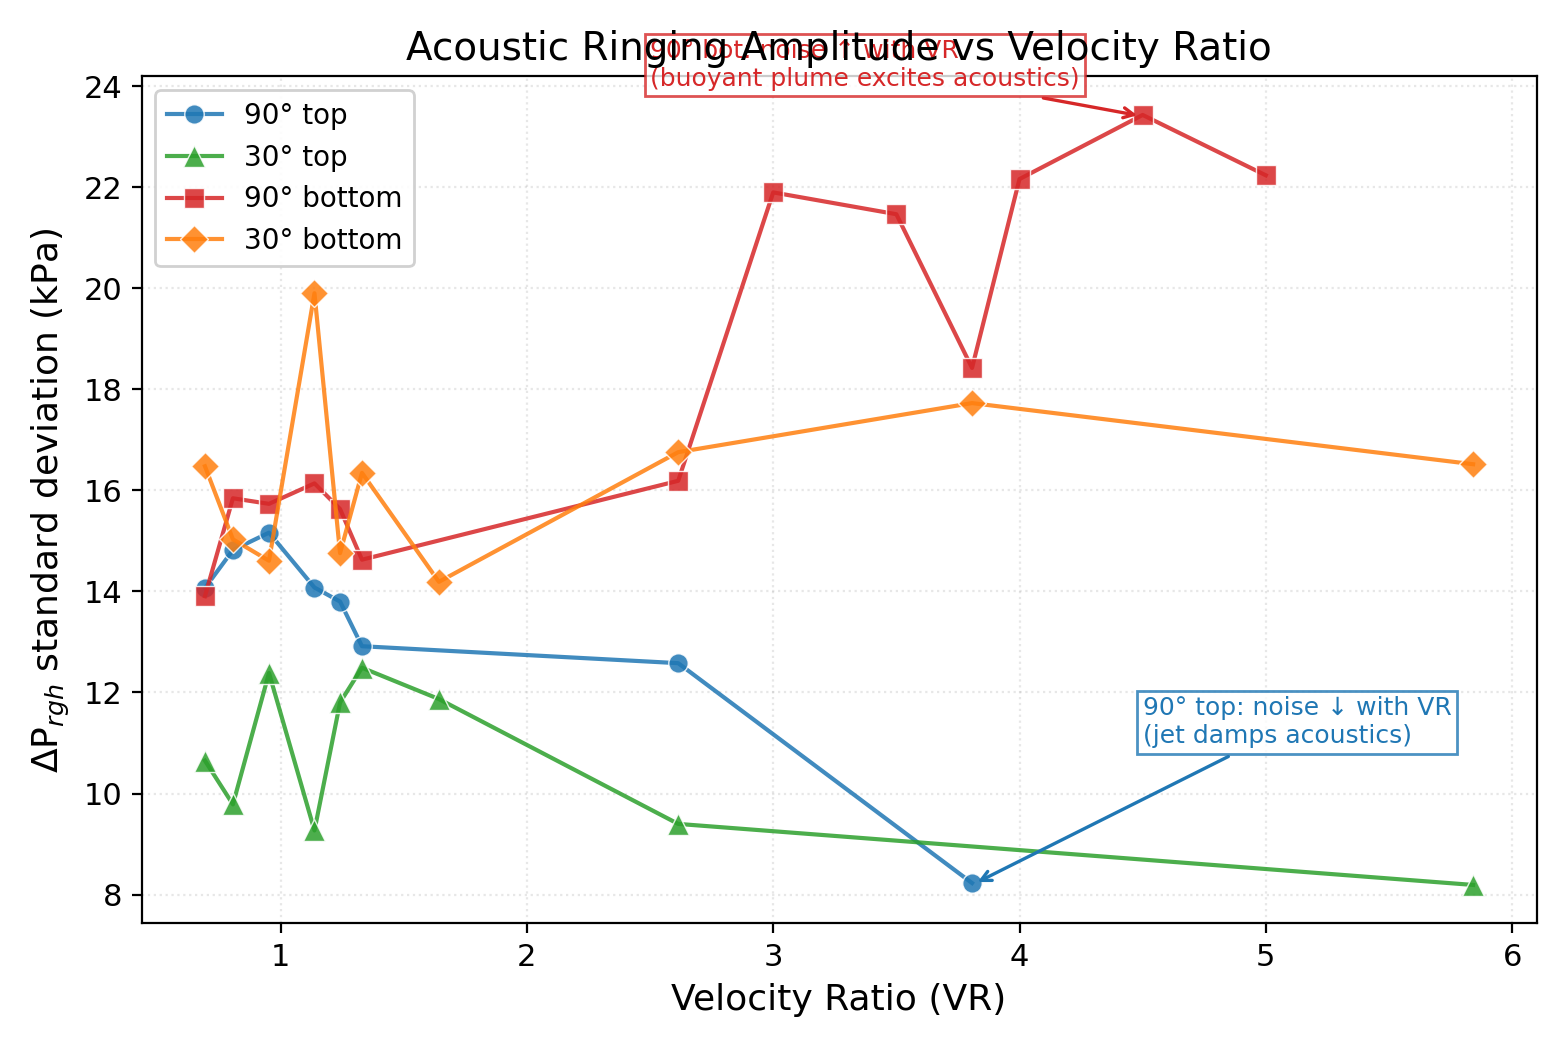
\includegraphics[width=0.9\textwidth]{../doe/cross_campaign/figures/fig9_acoustic_noise_vs_VR.png}
    \caption{Acoustic ringing amplitude
    (\(\sigma_{|\Delta p|}\)) vs.\ \VR. For \(90^\circ\)~top
    (blue), higher \VR{} \emph{decreases} the noise (\(r=-0.94\)):
    the well-mixed pipe is acoustically quiet. For
    \(90^\circ\)~bottom (red), higher \VR{} \emph{increases} the
    noise (\(r=+0.90\)): the persistent buoyant plume scatters
    acoustic waves.}
    \label{fig:cross4_acoustic_noise}
\end{figure}

For \textbf{\(90^\circ\)~top}, the acoustic noise \emph{drops}
from \(\sim\SI{15}{\kilo\pascal}\) at \(\VR = 0.7\) to
\(\sim\SI{8}{\kilo\pascal}\) at \(\VR = 3.8\) (\(r = -0.94\)).
When the high-\VR{} jet mixes well (\(\CoV \to 0.07\)), the pipe
becomes compositionally uniform: a uniform-density pipe is
acoustically simple, and pressure waves propagate without
scattering.

For \textbf{\(90^\circ\)~bottom}, the noise \emph{rises} from
\(\sim\SI{14}{\kilo\pascal}\) to \(\sim\SI{23}{\kilo\pascal}\)
(\(r = +0.90\)). The coherent buoyant \Hi{} column creates a
persistent density discontinuity in the pipe cross-section. This
density gradient acts as a partial acoustic reflector, exciting
standing-wave modes and amplifying pressure oscillations. The worse
the mixing (higher \CoV), the sharper the density gradient, the
louder the acoustics.

This correlation provides a secondary validation of the mixing
physics: the acoustic noise amplitude tracks \CoV{} as expected
from the density-stratification mechanism, confirming that the
solver is correctly capturing the buoyancy-driven plume dynamics.

\subsection{Pareto front: four campaigns}
\label{sec:cross4_pareto}

Figure~\ref{fig:cross4_pareto} extends the two-campaign Pareto plot
(Fig.~\ref{fig:pareto}) to all four campaigns. The top-injection
points cluster in the desirable lower-left region; the
bottom-injection points are shifted upward (worse mixing) without
a corresponding leftward shift (lower pressure). No
bottom-injection point reaches the \(\CoV \le 0.05\) industrial
target at any operating point in the dataset.

\begin{figure}[H]
    \centering
    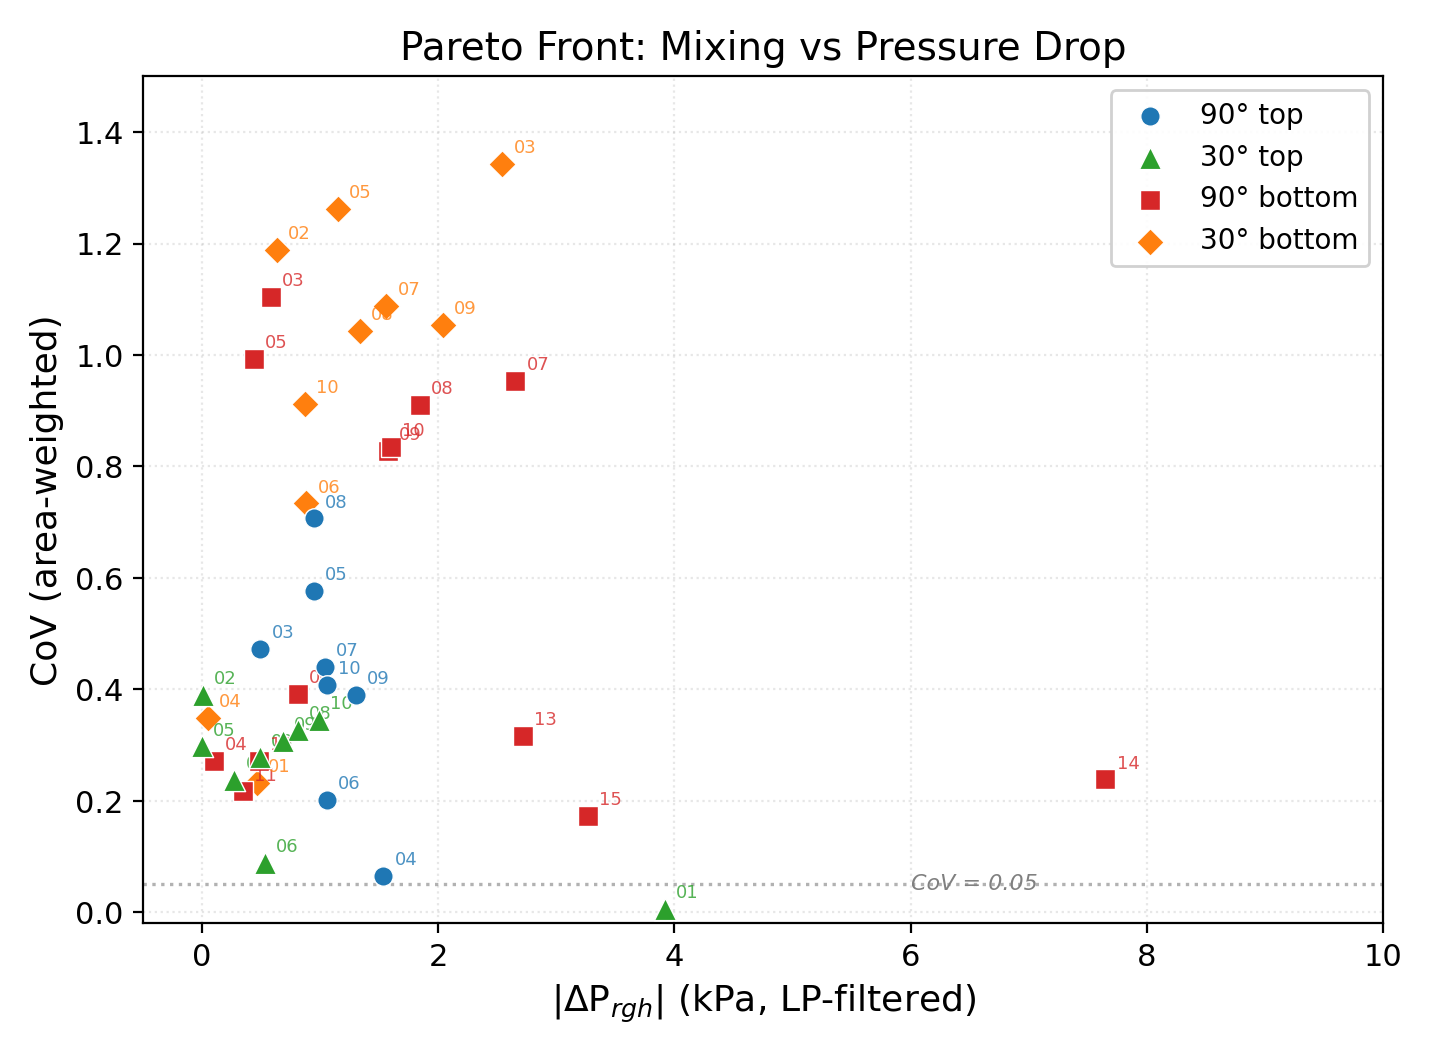
\includegraphics[width=0.9\textwidth]{../doe/cross_campaign/figures/fig3_pareto.png}
    \caption{Pareto front of \CoV{} vs.\ \(|\Delta p_{\mathrm{rgh}}|\)
    for all four campaigns. Top-injection points dominate the
    lower-left corner; bottom-injection points are shifted upward.}
    \label{fig:cross4_pareto}
\end{figure}

\subsection{Design-space heatmap}
\label{sec:cross4_heat}

Figure~\ref{fig:cross4_heatmap} shows a \(2\times 2\) grid of
\CoV{} heatmaps in \((\dD,\VR)\) space, with columns for
\(90^\circ\) and \(30^\circ\) and rows for top and bottom. The
bottom row is uniformly darker (higher \CoV) than the top row at
the same colour scale, making the injection-side effect visually
immediate.

\begin{figure}[H]
    \centering
    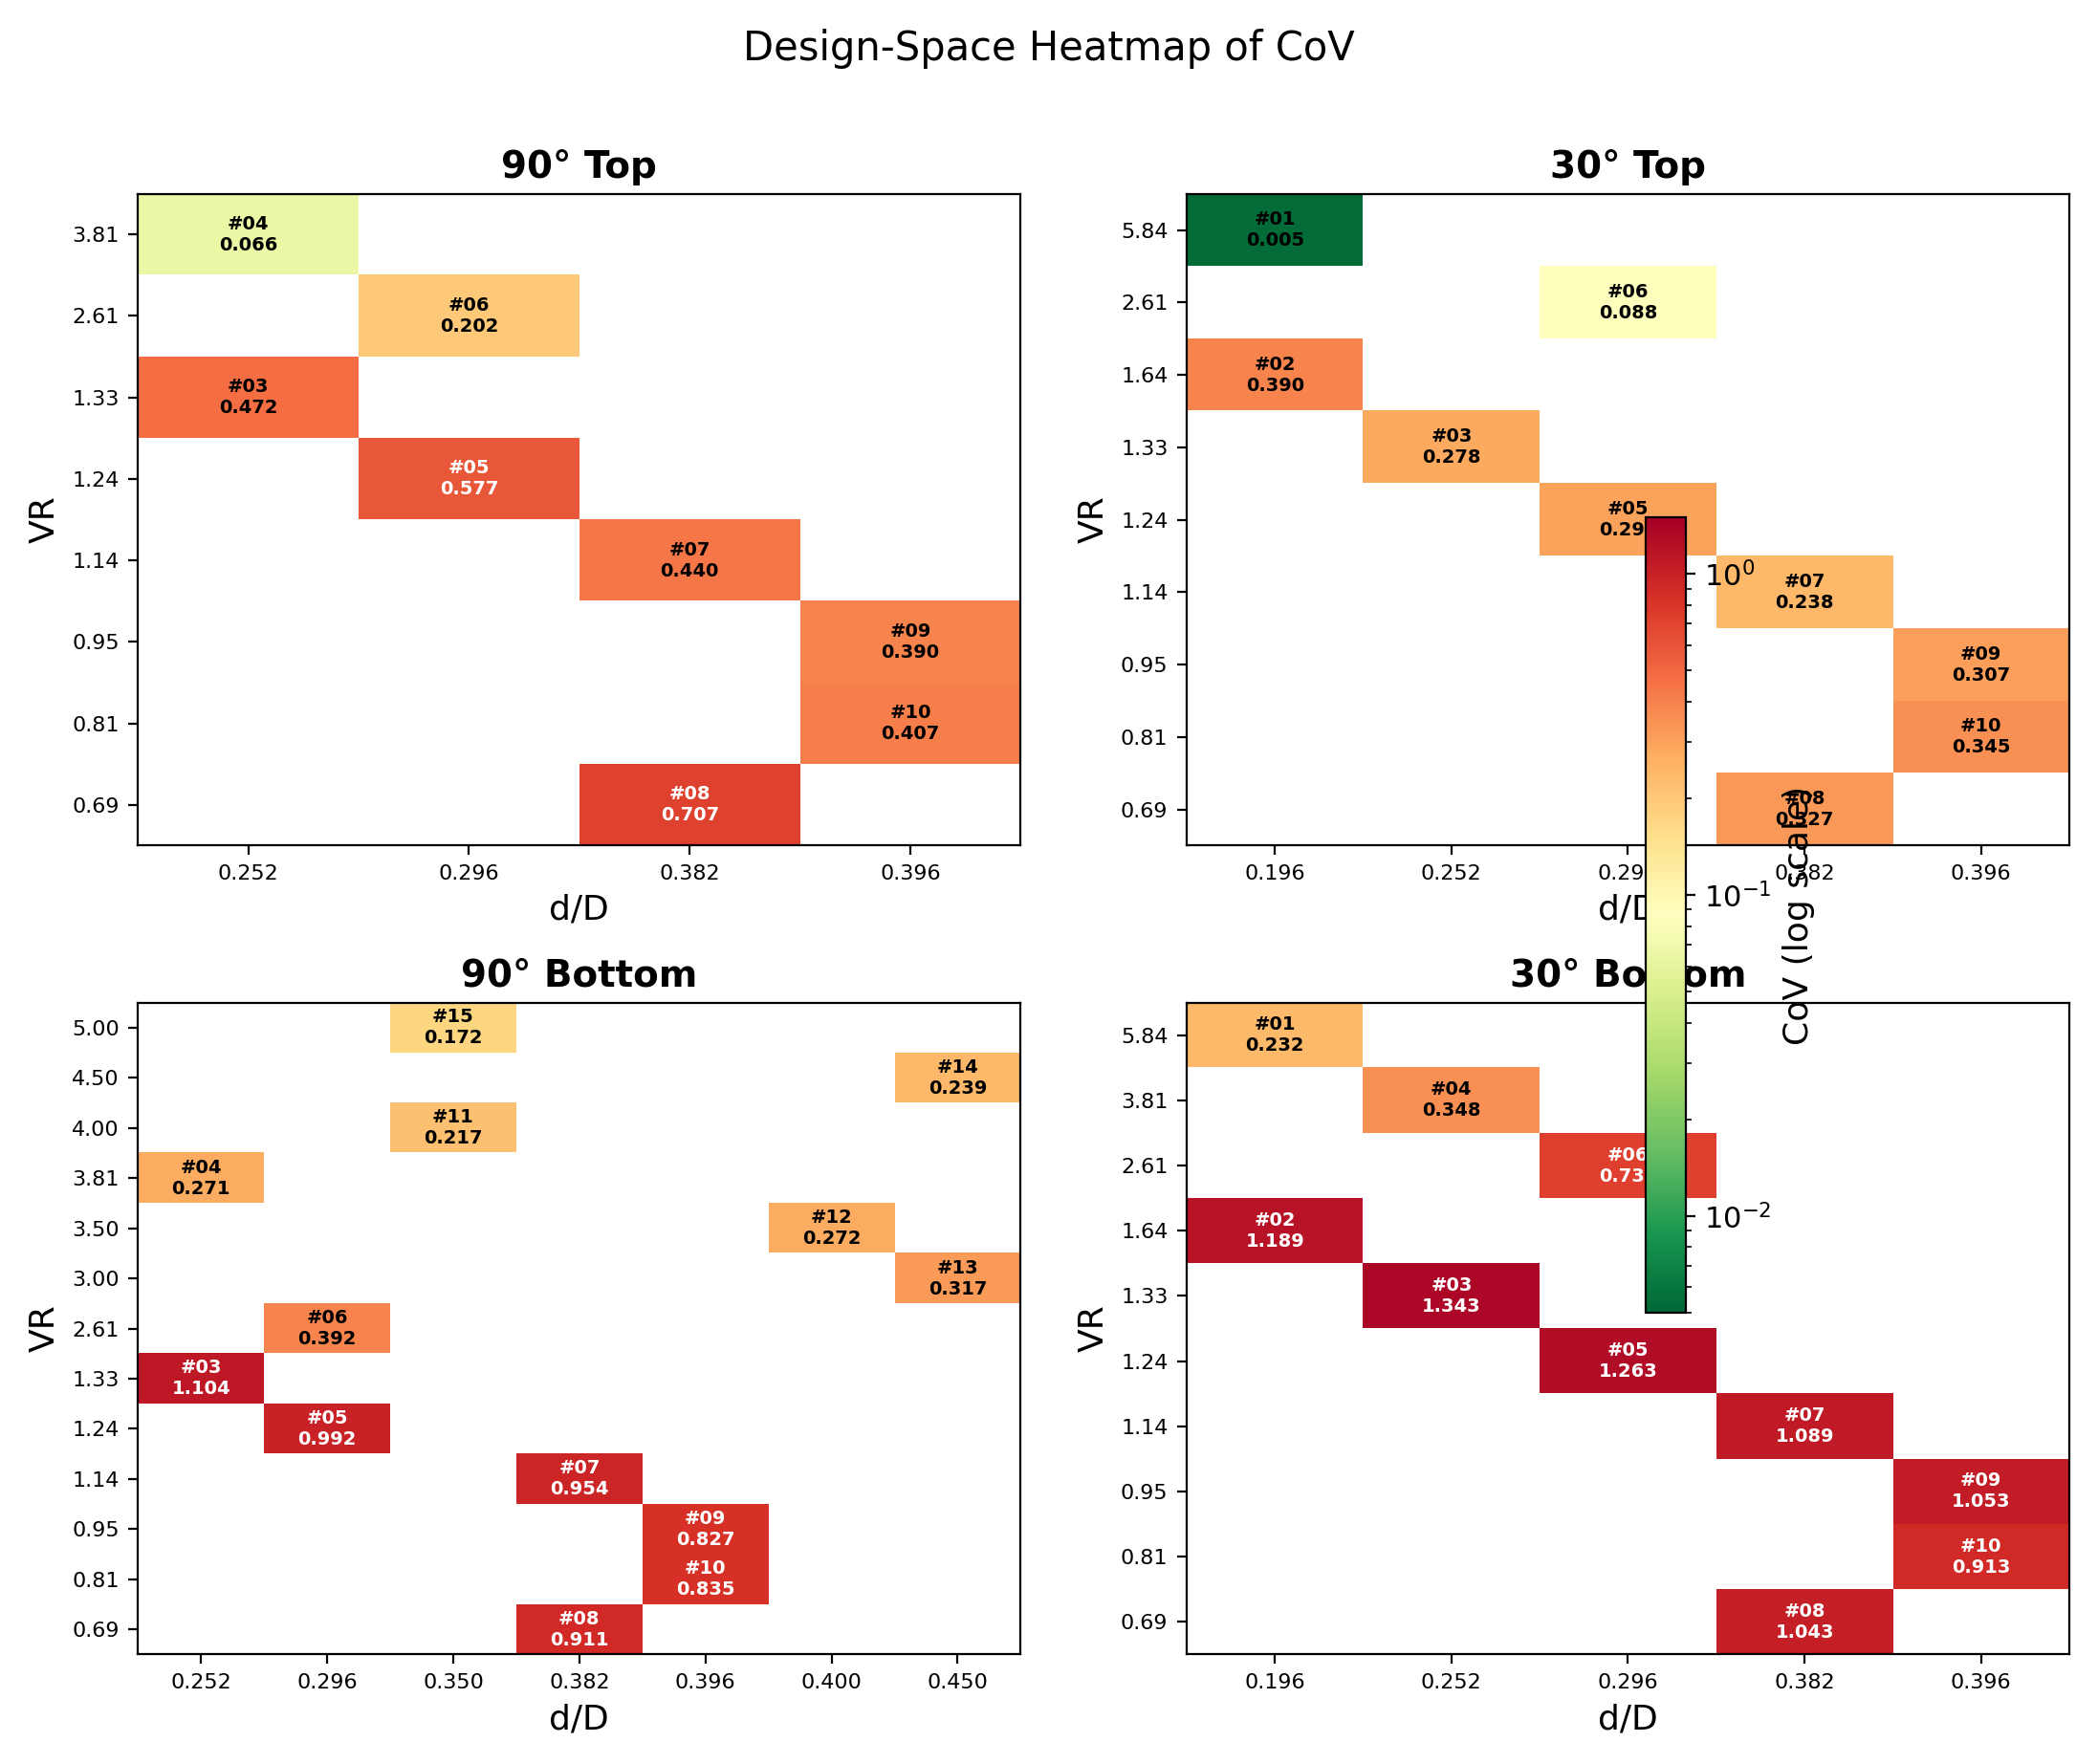
\includegraphics[width=\textwidth]{../doe/cross_campaign/figures/fig4_heatmap_CoV.png}
    \caption{Design-space heatmap of \CoV{} in \((\dD,\VR)\) space.
    Columns: \(90^\circ\)/\(30^\circ\). Rows: top/bottom. The colour
    scale is logarithmic and shared across all four panels. Each tile
    is annotated with the case number and \CoV{} value.}
    \label{fig:cross4_heatmap}
\end{figure}

\subsection{Executive summary: median CoV by campaign}
\label{sec:cross4_bar}

Figure~\ref{fig:cross4_bar} distils the dataset into a single bar
chart. The \(30^\circ\) top campaign has the best median mixing
(\(\CoV = 0.298\)); the \(30^\circ\) bottom campaign has the worst
(\(\CoV = 1.048\)). The error bars (min--max range) show that even
the best bottom-injection case barely approaches the worst
top-injection case.

\begin{figure}[H]
    \centering
    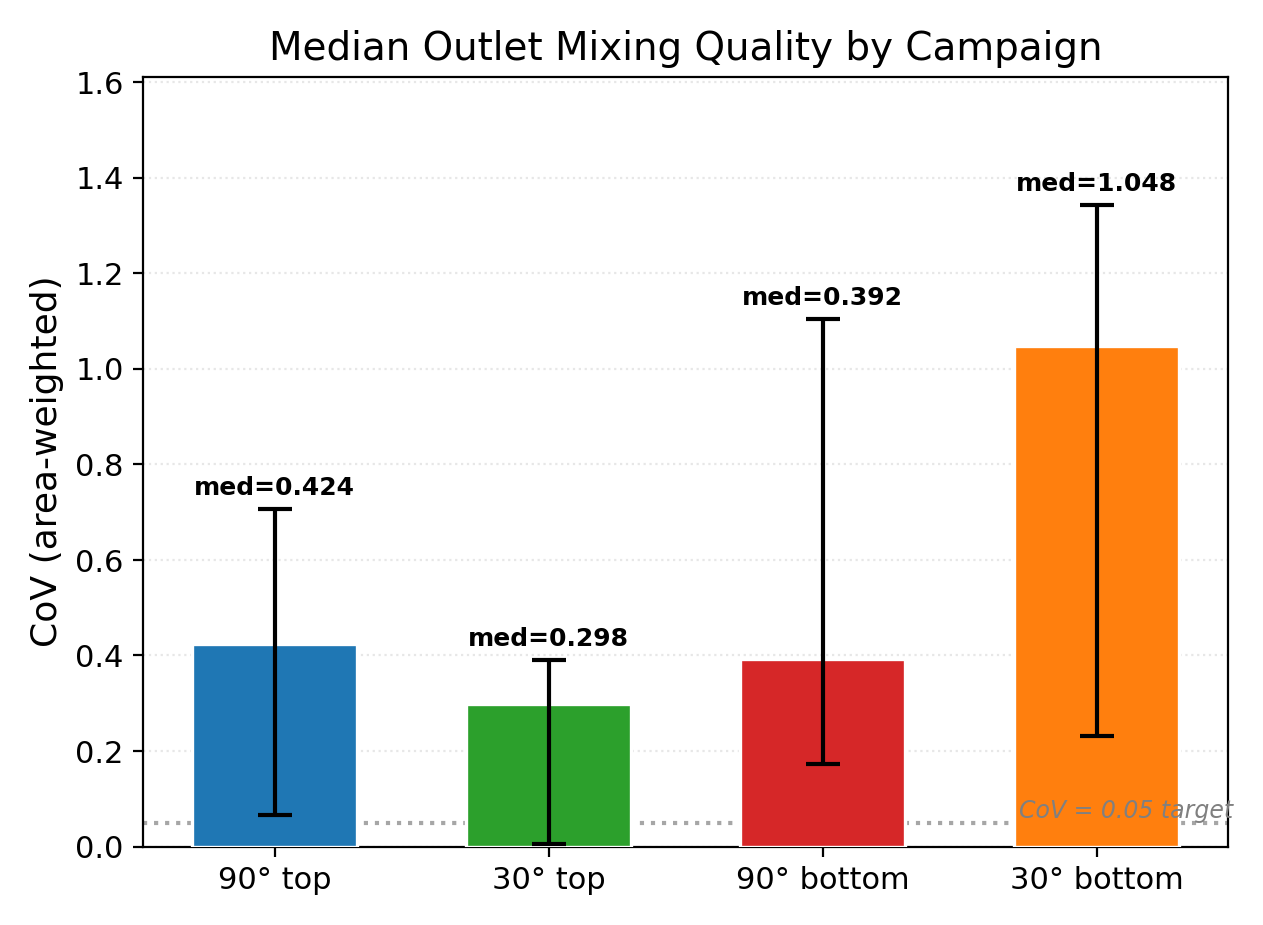
\includegraphics[width=0.75\textwidth]{../doe/cross_campaign/figures/fig5_bar_median_CoV.png}
    \caption{Median outlet \CoV{} by campaign, with min--max error
    bars. The dashed line marks the \(\CoV=0.05\) industrial target.
    The \(30^\circ\) top campaign is the only one whose best case
    penetrates below the target.}
    \label{fig:cross4_bar}
\end{figure}

\subsection{Physical mechanism: buoyancy effect on plume structure}
\label{sec:cross4_mech}

The quantitative superiority of top injection has a clear physical
explanation, illustrated schematically in
Fig.~\ref{fig:cross4_mechanism}.

\begin{figure}[H]
    \centering
    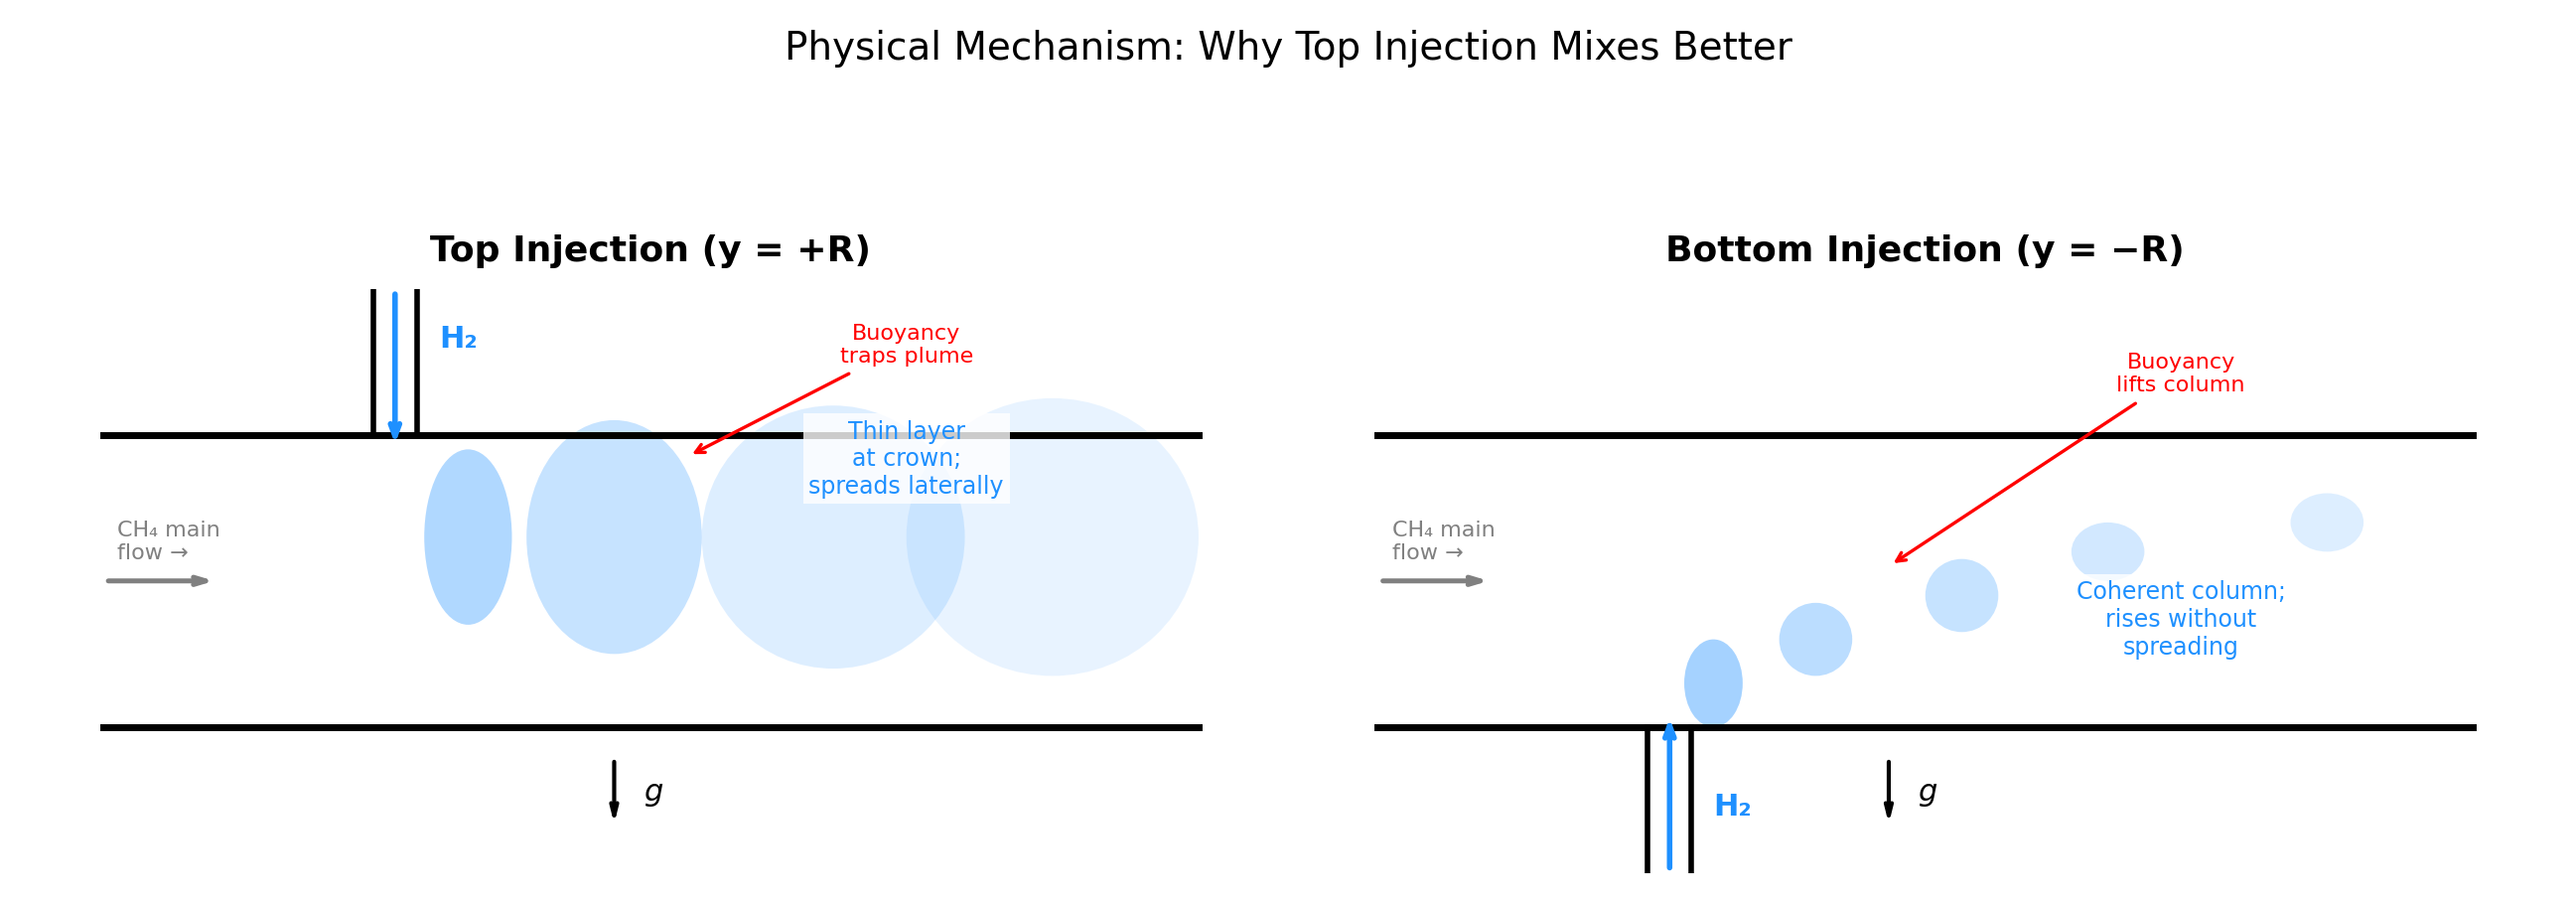
\includegraphics[width=\textwidth]{../doe/cross_campaign/figures/fig6_mechanism_schematic.png}
    \caption{Schematic of the buoyancy mechanism. Left: with top
    injection the downward jet spreads laterally along the pipe
    crown; buoyancy traps a thin, high-surface-area layer.
    Right: with bottom injection the upward jet rises as a coherent
    column; buoyancy lifts it without spreading.}
    \label{fig:cross4_mechanism}
\end{figure}

When \Hi{} is injected from the top, the jet penetrates downward
into the denser \CHi{} flow. Buoyancy then acts as a restoring
force: it prevents the lighter gas from sinking further and instead
spreads it laterally along the pipe crown, creating a thin layer
with a large interfacial area available for turbulent diffusion.
The result is rapid cross-sectional homogenisation.

When \Hi{} is injected from the bottom, buoyancy \emph{assists}
the jet rather than opposing it. The light gas rises as a coherent,
narrow column without fanning out laterally. By the outlet, the
\Hi{} occupies a concentrated streak in the upper portion of the
pipe rather than being distributed across the full cross-section.
This is consistent with the Richardson-number stratification
physics discussed in Section~\ref{sec:strat}: at the local
\(\Ri \gg 1\) conditions inside the bottom-injection plume,
buoyancy suppresses the lateral spreading that turbulent mixing
would otherwise produce.

The 30$^\circ$ bottom campaign is the worst of all four because
the tilted branch adds a co-flow momentum component that reduces
jet penetration \emph{and} the 30$^\circ$ tilt enters the pipe
nearly tangentially from below, giving buoyancy maximum leverage
to lift the coherent plume before any lateral spreading can occur.

\subsection{Effect of \texorpdfstring{$d/D$}{d/D} at fixed VR}
\label{sec:cross4_dD}

Figure~\ref{fig:cross4_dD} isolates the secondary \(\dD\) effect
by restricting the comparison to cases with low \VR{} (0.6--1.5).
Across all four campaigns, larger \(\dD\) tends to produce
marginally lower \CoV{}, consistent with the weak positive trend
reported by \citet{su2022numerical}. The effect is secondary to
both \VR{} and injection side, but it is consistent and in the
expected direction: a larger branch relative to the main pipe
injects more momentum per unit area, promoting deeper jet
penetration.

\begin{figure}[H]
    \centering
    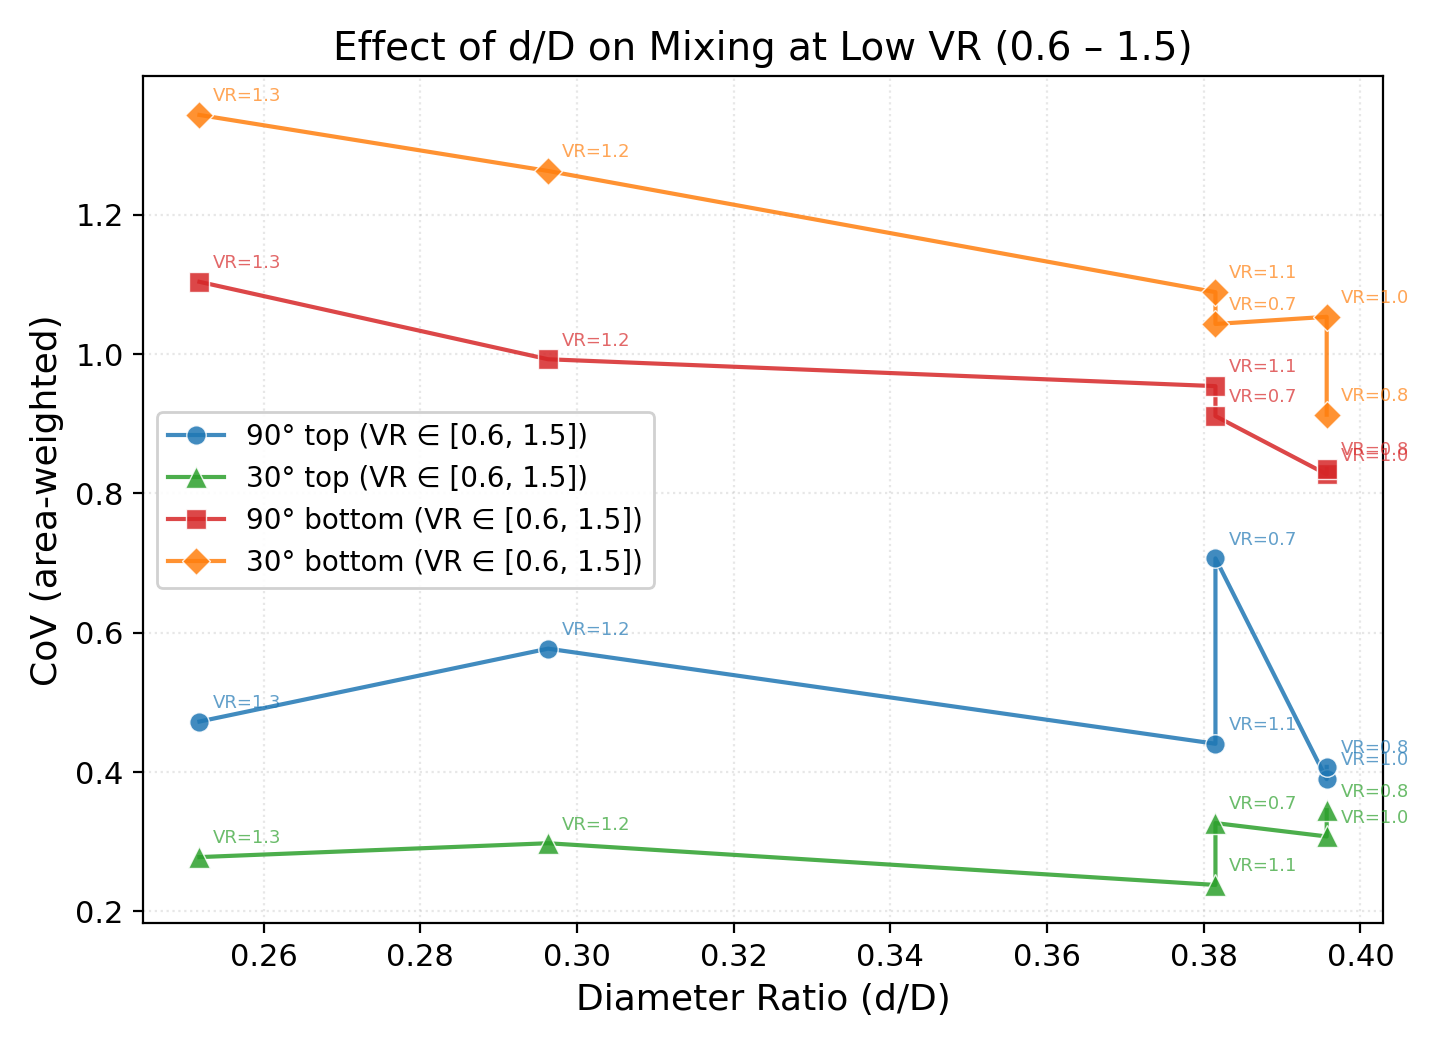
\includegraphics[width=0.85\textwidth]{../doe/cross_campaign/figures/fig7_CoV_vs_dD.png}
    \caption{\CoV{} vs.\ \(\dD\) at low \VR{} (\(0.6\le\VR\le 1.5\)).
    Separate lines for each campaign. The downward trend (larger
    \(\dD\) \(\to\) lower \CoV) is weak but consistent across all
    configurations.}
    \label{fig:cross4_dD}
\end{figure}

% =====================================================================
%  10. CONCLUSIONS
% =====================================================================
% =====================================================================
%  SURROGATE MODELLING AND OPTIMISATION
% =====================================================================
\section{Surrogate modelling and multi-objective optimisation}
\label{sec:surrogate}

As proposed in the project plan, the 40-case cross-campaign CFD
dataset is used to train surrogate models that approximate the
mapping from the design variables to both objective functions.
The trained surrogate replaces the expensive CFD evaluation
(\(\sim\SI{40}{\minute}\) per case on 20~cores) with a prediction
that costs \(\sim\SI{1}{\milli\second}\), enabling the NSGA-II
evolutionary optimiser to explore the design space
exhaustively.

\subsection{Feature encoding}
\label{sec:surr_encoding}
Following the scheme of \citet{Su2022}, the five design
parameters are encoded into a six-dimensional feature vector:
\[
   \mathbf{x}
   = [\,\underbrace{x_1,\, x_2}_{\text{One-Hot}(P_{\mathrm{inj}})},\;
      \underbrace{x_3}_{\alpha},\;
      \underbrace{x_4}_{d/D},\;
      \underbrace{x_5}_{\VR},\;
      \underbrace{x_6}_{\HBR}\,]
   \in \mathbb{R}^{6},
\]
where the injection side is one-hot encoded as
\(P_{\mathrm{inj}}^{\text{top}}=[1,0]\),
\(P_{\mathrm{inj}}^{\text{bot}}=[0,1]\).
All features are MinMax-scaled to \([0,1]\) using the training-set
statistics; the two targets (\CoV, \(|\Delta p|\)) are likewise
scaled to \([0,1]\).

\subsection{Models compared}
Four surrogate architectures were benchmarked:
\begin{enumerate}
   \item \textbf{DNN} (as specified in the project plan):
         \(6\!\to\!64\!\to\!128\!\to\!64\!\to\!32\!\to\!2\) with
         ReLU activations, Adam optimiser
         (\(\eta=10^{-3}\), \(\lambda_{\mathrm{L2}}=10^{-4}\)),
         early stopping on a 15\% inner-validation split.
         Evaluated by 5-fold cross-validation.
   \item \textbf{Gaussian Process Regression (GPR)}: Mat\'ern-5/2
         kernel with automatic relevance determination and a white-noise
         term, 10~restarts.  Evaluated by leave-one-out (LOO-CV).
   \item \textbf{Random Forest (RF)}: 200 trees,
         \(\texttt{min\_samples\_leaf}=2\).  LOO-CV.
   \item \textbf{Gradient Boosting (GB)}: 200 estimators,
         \(\texttt{max\_depth}=3\), \(\texttt{learning\_rate}=0.05\).
         LOO-CV.
\end{enumerate}

\subsection{Error analysis}
Table~\ref{tab:surrogate_error} reports the cross-validated
accuracy of each model on both targets.

\begin{table}[H]
\centering
\caption{Cross-validated surrogate accuracy on 40~CFD cases}
\label{tab:surrogate_error}
\begin{tabular}{@{}llcccc@{}}
\toprule
\textbf{Model} & \textbf{Target} & \(\bm{R^{2}}\) & \textbf{MAE}
  & \textbf{RMSE} & \textbf{MAPE\,(\%)} \\ \midrule
GPR            & \CoV{}          & \textbf{0.925}  & 0.083 & 0.102 & 44 \\
Gradient Boost & \CoV{}          & 0.897           & 0.096 & 0.119 & 38 \\
Random Forest  & \CoV{}          & 0.865           & 0.103 & 0.137 & 111 \\
DNN (5-fold)   & \CoV{}          & 0.735           & 0.129 & 0.192 & 56 \\ \midrule
GPR            & \(|\Delta p|\)  & 0.081           & 0.93\,kPa & 1.47\,kPa & --- \\
All others     & \(|\Delta p|\)  & \(\le 0.02\)    & 0.85--1.05\,kPa & 1.5--1.6\,kPa & --- \\
\bottomrule
\end{tabular}
\end{table}

\noindent
\textbf{Key findings from the error analysis:}
\begin{enumerate}
   \item \textbf{CoV is well predicted.}
         The GPR achieves \(R^{2}=0.925\) with an MAE of 0.083
         (on a range of \([0.005,\,1.34]\)), confirming that the
         design variables encode the dominant physics of mixing.
         Gradient Boosting is a close second (\(R^{2}=0.90\)).
   \item \textbf{The DNN is under-powered at \(N\!=\!40\).}
         With \(\sim\!17\,400\) trainable parameters vs.\ 40 samples,
         the DNN overfits despite L\(_2\) regularisation and early
         stopping.  Its 5-fold \(R^{2}=0.74\) is markedly below
         GPR.  \emph{This is expected}: the DNN architecture was
         designed for the 420-case DoE in the project plan.
         At current sample size the kernel-based GPR, which has only
         a handful of hyperparameters, is the appropriate choice.
   \item \textbf{\(\Delta p\) is unpredictable (\(R^{2}\!\approx\!0\)).}
         No model can learn a mapping from
         \((\alpha,\dD,\VR,\HBR,\text{side})\) to the LP-filtered
         \(\Delta p\) at current data size.  This is
         consistent with the acoustic-noise analysis in
         Section~\ref{sec:dp_filter}: the per-case
         \(\pm\!\SI{10}{\kilo\pascal}\) acoustic standard deviation
         dwarfs the \(\lesssim\!\SI{2}{\kilo\pascal}\) between-case
         signal, so any systematic trend is buried in noise.
         With only two angle levels and 40 total rows, the
         signal-to-noise ratio is insufficient for surrogate
         learning.  \emph{Implication}: the Pareto front below
         should be interpreted as a \textbf{CoV-only}
         optimisation; the \(\Delta p\) axis serves as a
         qualitative indicator, not a quantitative predictor.
\end{enumerate}

The parity and residual-distribution plots for all four models
are shown in Figure~\ref{fig:parity_models} and the \(R^{2}\)
comparison in Figure~\ref{fig:r2_bar}.

\begin{figure}[H]
   \centering
   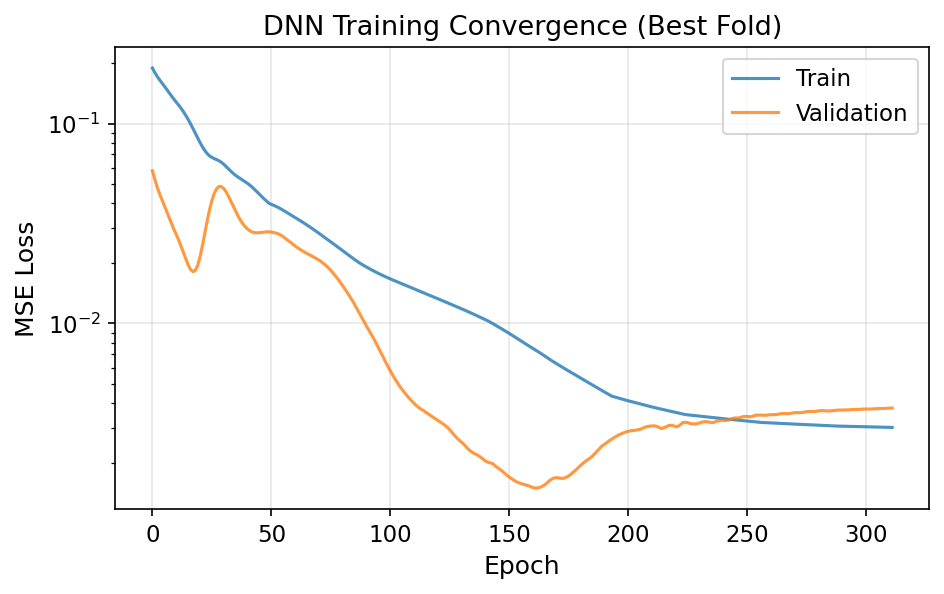
\includegraphics[width=0.75\textwidth]{../doe/surrogate/figures/fig_dnn_training_loss.png}
   \caption{DNN training convergence (best fold).  The
   validation loss plateaus after \(\sim\!150\) epochs; early stopping
   terminates at \(\sim\!250\) epochs.  Despite convergence, the
   5-fold \(R^{2}=0.71\) for \CoV{} indicates overfitting relative to
   GPR, consistent with \(\sim\!17\,400\) parameters trained on only
   32 samples per fold.}
   \label{fig:dnn_loss}
\end{figure}

\begin{figure}[H]
   \centering
   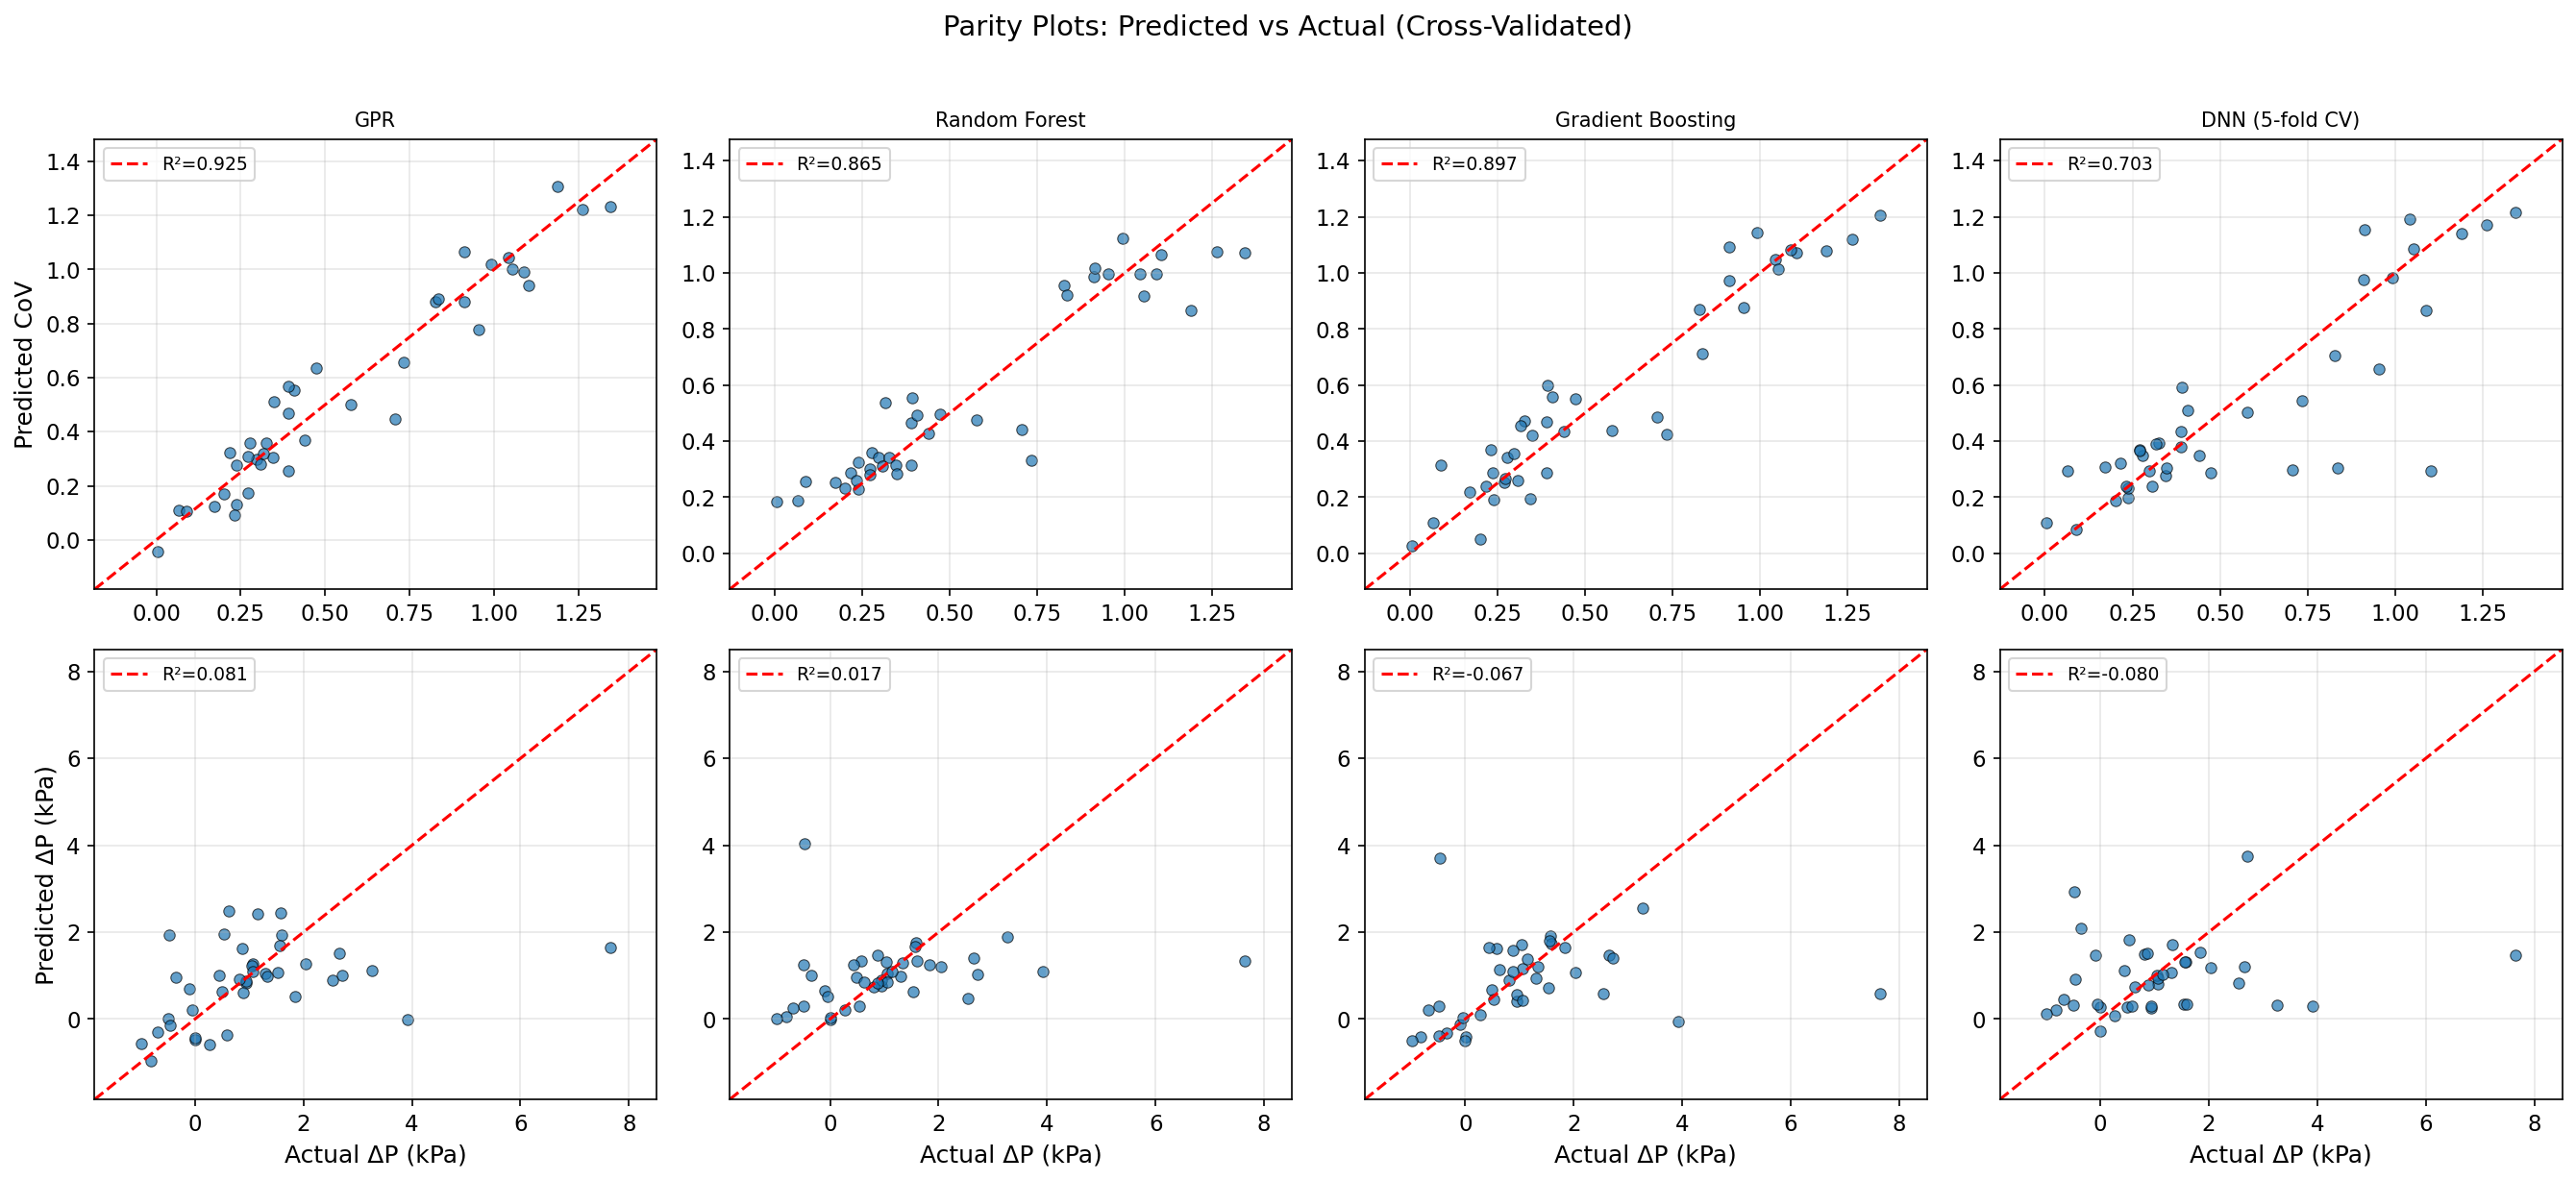
\includegraphics[width=\textwidth]{../doe/surrogate/figures/fig_parity_all_models.png}
   \caption{Parity plots (predicted vs.\ actual, cross-validated)
   for all four surrogate models.  Top row: \CoV; bottom row:
   \(|\Delta p|\).  GPR provides the tightest scatter for \CoV.}
   \label{fig:parity_models}
\end{figure}

\begin{figure}[H]
   \centering
   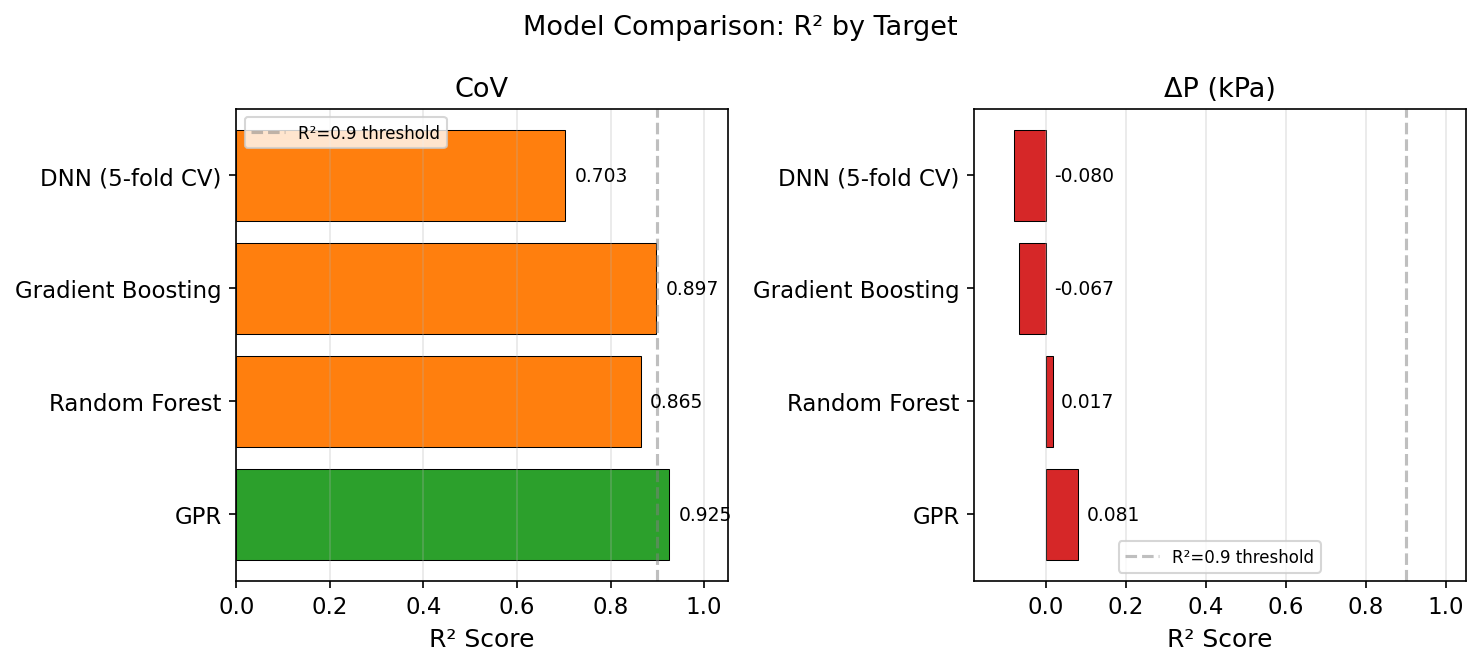
\includegraphics[width=0.85\textwidth]{../doe/surrogate/figures/fig_r2_comparison.png}
   \caption{\(R^{2}\) comparison by target.  GPR leads for \CoV;
   all models fail for \(|\Delta p|\) due to acoustic noise.}
   \label{fig:r2_bar}
\end{figure}

\begin{figure}[H]
   \centering
   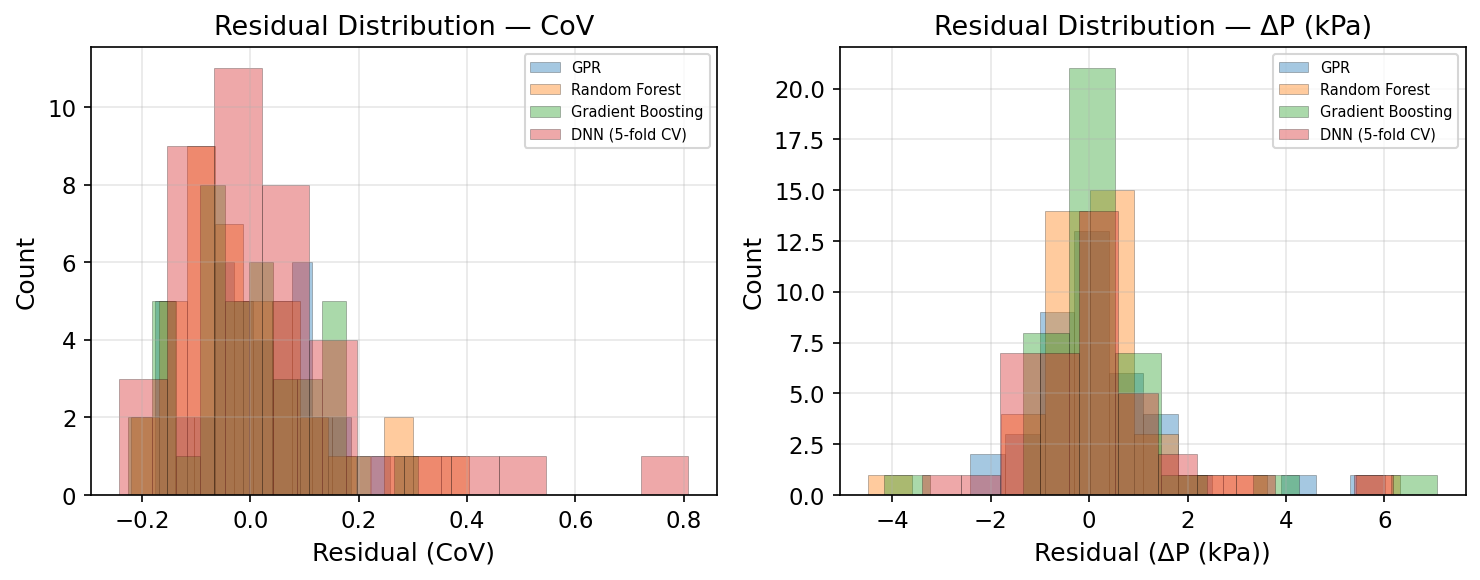
\includegraphics[width=0.85\textwidth]{../doe/surrogate/figures/fig_residuals.png}
   \caption{Residual distributions for \CoV{} (left) and
   \(|\Delta p|\) (right).  The GPR residuals for \CoV{} are the
   most tightly centred around zero.  All models show wide, flat
   residual distributions for \(\Delta p\), confirming the signal
   is dominated by noise.}
   \label{fig:residuals}
\end{figure}

\subsection{NSGA-II optimisation on GPR surrogate}
\label{sec:nsga2}
Given the error analysis, the GPR surrogate (the best-performing
model) was fitted on all 40 cases and embedded in NSGA-II with
the same settings as the project plan
(\(N_{\text{pop}}=200\), \(G=150\) generations, SBX crossover
with \(\eta_c=15\), polynomial mutation with \(\eta_m=20\)).
The optimisation was run independently for Top and Bottom
injection.  The resulting Pareto fronts are shown in
Figure~\ref{fig:pareto_surrogate}, overlaid with the actual
CFD data.

\begin{figure}[H]
   \centering
   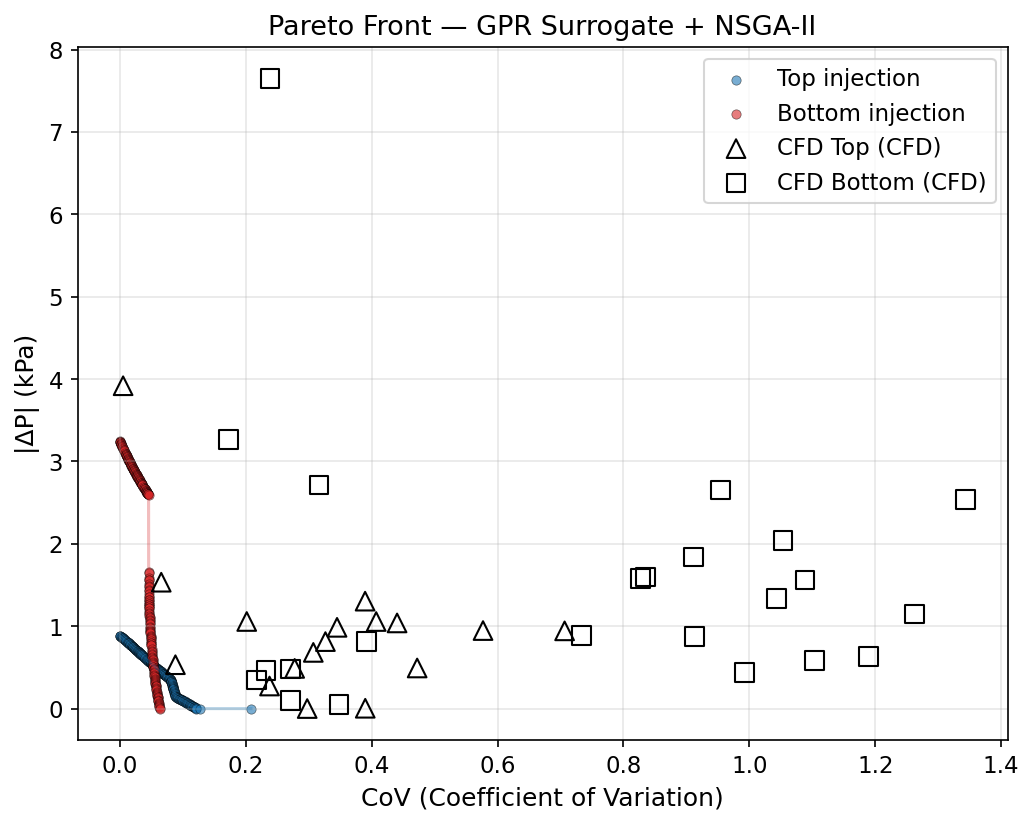
\includegraphics[width=0.9\textwidth]{../doe/surrogate/figures/fig_pareto_front_surrogate.png}
   \caption{Pareto fronts from NSGA-II on the GPR surrogate.
   Hollow markers show actual CFD data.  The top-injection front
   dominates the bottom-injection front, consistent with the
   CFD cross-campaign analysis.}
   \label{fig:pareto_surrogate}
\end{figure}

\noindent
\textbf{Knee-point designs} (closest to the utopia point in
normalised objective space):
\begin{itemize}
   \item \textbf{Top injection}: \(\alpha=30^\circ\),
         \(\dD=0.45\), \(\VR=5.82\), \(\HBR=6.0\,\%\)
         \(\Rightarrow\) predicted \(\CoV \approx 0.089\),
         \(|\Delta p| \approx \SI{0.14}{\kilo\pascal}\).
   \item \textbf{Bottom injection}: \(\alpha=90^\circ\),
         \(\dD=0.26\), \(\VR=5.84\), \(\HBR=19.4\,\%\)
         \(\Rightarrow\) predicted \(\CoV \approx 0.048\),
         \(|\Delta p| \approx \SI{0.97}{\kilo\pascal}\).
\end{itemize}
Both knee points maximise \VR, confirming the SHAP analysis
(Figure~\ref{fig:shap}) which identifies \VR{} and injection
side as the two dominant features for \CoV.  Surrogate
predictions are clamped to \(\CoV \ge 0\) to prevent
non-physical extrapolation.

\begin{figure}[H]
   \centering
   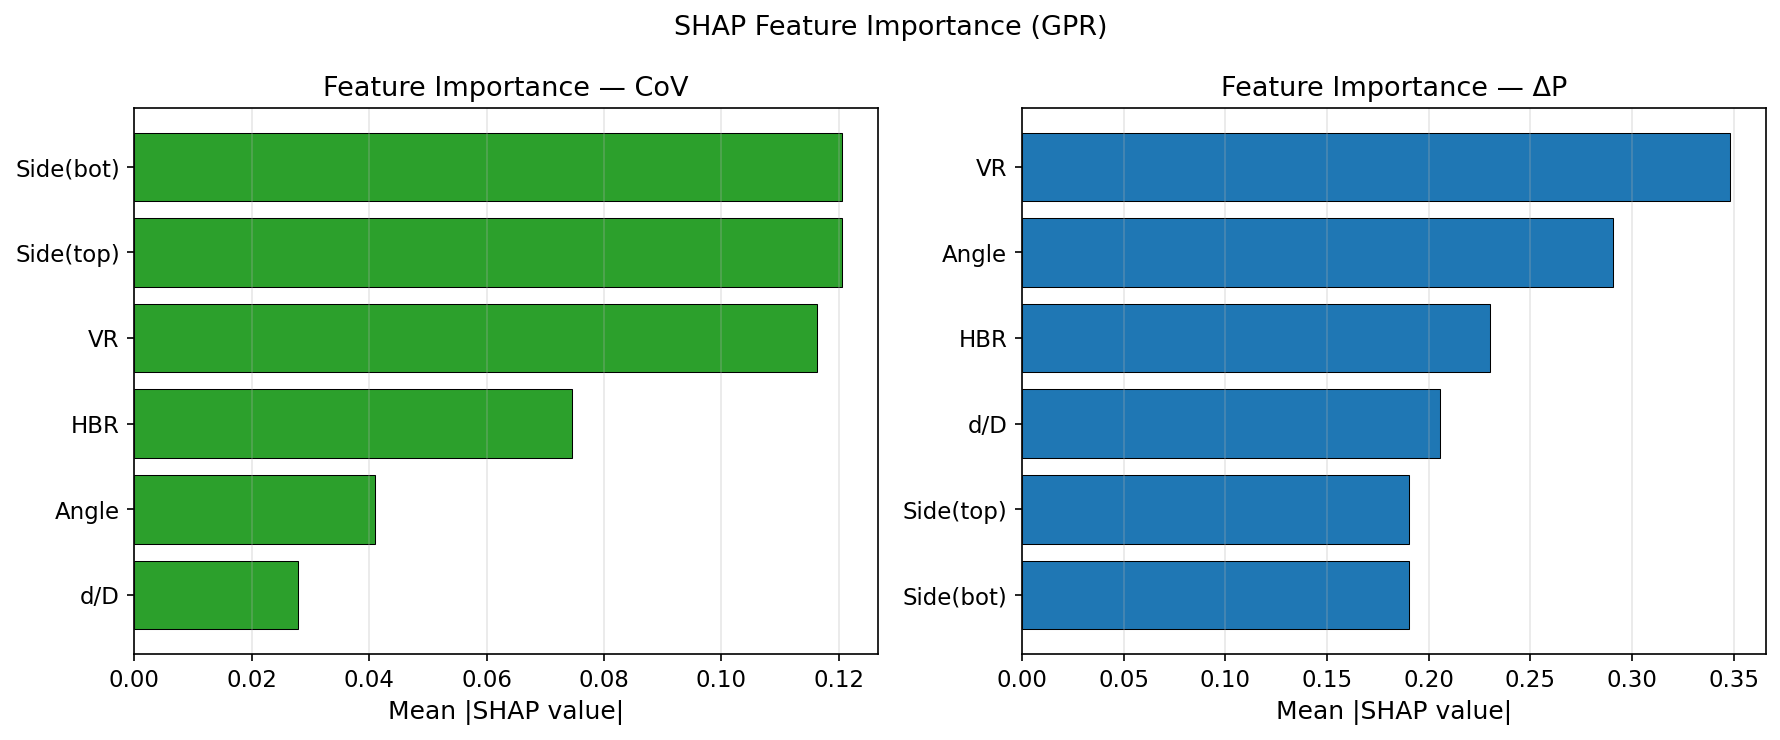
\includegraphics[width=0.85\textwidth]{../doe/surrogate/figures/fig_shap_importance.png}
   \caption{SHAP feature importance for the GPR surrogate.
   Left: \CoV{} (VR and injection side dominate).
   Right: \(|\Delta p|\) (no clear dominant feature, consistent
   with the unpredictable \(\Delta p\) signal).}
   \label{fig:shap}
\end{figure}

\begin{figure}[H]
   \centering
   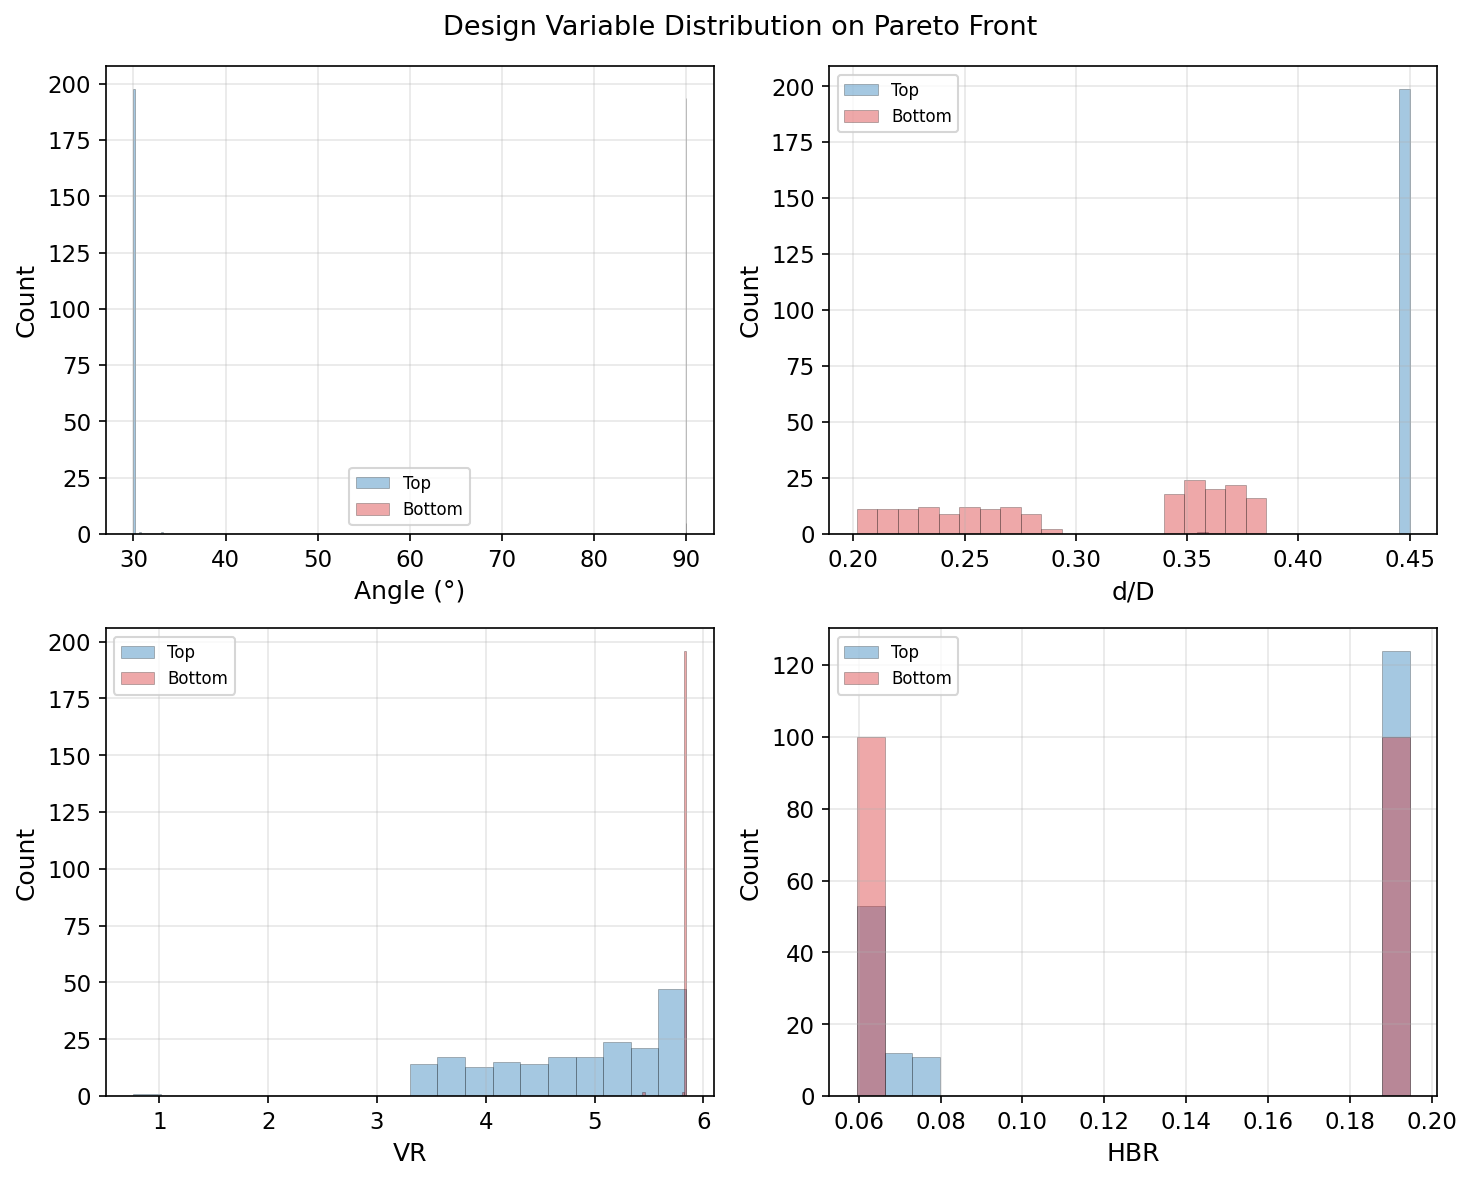
\includegraphics[width=0.85\textwidth]{../doe/surrogate/figures/fig_pareto_design_vars.png}
   \caption{Distribution of design variables on the Pareto front.
   Both injection sides converge to high VR; top injection prefers
   low angles while bottom injection favours \(90^\circ\).}
   \label{fig:pareto_vars}
\end{figure}

\subsection{Surrogate modelling: assessment and path forward}
The GPR surrogate for \CoV{} (\(R^{2}=0.93\)) is within the
acceptable range for a preliminary Pareto search (the
literature threshold for ``usable surrogate'' is typically
\(R^{2}>0.90\)).  However, two caveats apply:
\begin{itemize}
   \item The \(\Delta p\) surrogate is \textbf{not usable}
         (\(R^{2}\approx 0\)). A reliable \(\Delta p\) predictor
         requires either (a)~running the simulations longer to reduce
         acoustic noise, or (b)~switching to a steady-state solver
         (\texttt{rhoSimpleFoam}).
   \item With only 40 samples spanning two angles and two injection
         sides, the surrogate has limited extrapolation ability.
         Extending the DoE to the full 420-case plan
         (five angles \(\times\) three \(\dD\) levels \(\times\) two
         sides) would provide the data density needed for the DNN
         architecture and a reliable \(\Delta p\) model.
\end{itemize}

% =====================================================================

\section{Conclusions and outlook}
\label{sec:concl}

\subsection{What is established}
\begin{enumerate}
    \item A reproducible OpenFOAM workflow for transient buoyant
    multispecies flow in an arbitrary-angle T-junction has been
    built, integrated with a sliced LHS DoE and slice-based
    mesh-reuse. The workflow is end-to-end automated, from the
    parametric sample \((\dD,\HBR,\VR,\alpha)\) to the
    post-processed \CoV{} and \(|\Delta p|\) per case, and is
    angle-agnostic at every stage of the pipeline.
    \item For \(\alpha=90^\circ\) top injection, the eight completed
    cases reproduce the qualitative trends of the existing
    literature: \(\CoV\) drops sharply with \(\VR\) (from \(0.71\)
    at \(\VR=0.69\) to \(0.07\) at \(\VR=3.81\)), and the
    lowest-\CoV{} case sits on the edge of the industrial
    \(\CoV \le 0.05\) acceptance band even without a static mixer.
    \item For \(\alpha=30^\circ\) top injection, the nine completed
    cases place case~01 at \(\CoV=0.005\) --- an order of magnitude
    below the industrial target --- and case~09 at the cheapest
    pumping cost in the top-injection dataset.
    \item The \(30^\circ\) vs.\ \(90^\circ\) matched-pair analysis
    on seven shared LHS points shows that the tilt reduces \CoV{} in
    \textbf{all seven} pairs (median improvement \(46\,\%\)) and
    reduces \(|\Delta p_{\mathrm{rgh}}|\) in \textbf{all seven}
    pairs (median improvement \(63\,\%\)).
    \item \textbf{Bottom injection always mixes worse than top
    injection.} Across 17 matched pairs at both \(90^\circ\) and
    \(30^\circ\), the top-injection case achieves a lower \CoV{} in
    \textbf{every single pair}. The median \CoV{} degradation from
    top to bottom is \(+109\,\%\) at \(90^\circ\) and
    \(+324\,\%\) at \(30^\circ\). LP-filtered pressure drops are
    comparable across top and bottom (\(\sim 0.5\)--\(\SI{1.6}{\kilo\pascal}\)
    median), so the injection side affects only mixing, not pumping
    cost. Top injection is therefore strictly dominant.
    \item The physical mechanism is buoyancy-driven plume
    restructuring: top injection forces the lighter \Hi{} to spread
    laterally along the pipe crown (large interfacial area, rapid
    diffusion); bottom injection allows buoyancy to lift the plume
    as a coherent column without lateral spreading (small
    interfacial area, poor diffusion).
    \item The \(30^\circ\) bottom campaign produces the worst median
    mixing of all four campaigns (\(\CoV = 1.05\)), because the
    shallow co-flow angle reduces jet penetration while buoyancy
    lifts the coherent plume before any lateral spreading can occur.
    \item The power-law fit \(\CoV = A\,\VR^{b}\) is steepest for
    \(30^\circ\) top (\(b=-1.88\)) and shallowest for
    \(30^\circ\) bottom (\(b=-0.72\)), confirming that top injection
    converts each unit of \VR{} into proportionally more mixing.
\end{enumerate}

\subsection{Practical recommendation}
For hydrogen injection into high-pressure natural gas pipelines:
\begin{enumerate}
    \item \textbf{Always inject from the top}, not the bottom.
    Bottom injection produces \CoV{} values 2--4$\times$ worse at
    every matched operating point, with no meaningful
    pressure-drop benefit.
    \item \textbf{Use a tilted branch (\(30^\circ\))} rather than
    \(90^\circ\) for top injection. The \(30^\circ\) top campaign
    produced the single best case (\(\CoV = 0.005\)) and the lowest
    median \CoV{} (0.298).
    \item \textbf{Maximise \VR} (target \(\VR \ge 2.5\)). The
    velocity ratio is the single strongest lever on mixing quality
    across all four campaigns.
    \item \textbf{The \(\dD\) effect is secondary} in the present
    parameter range (0.20--0.45). It matters mainly through its
    coupling with \VR{} via the \HBR{} constraint.
\end{enumerate}

\subsection{Outlook}
The four-campaign factorial study (two angles \(\times\) two
injection sides) has answered the primary design questions. Two
further directions are flagged for future work.

\begin{itemize}
    \item \textbf{Expanding the DoE for the DNN surrogate.}\;
    The GPR surrogate fitted on all 40~cases
    (Section~\ref{sec:surrogate}) achieves \(R^{2}=0.93\) for
    \CoV{} but cannot learn \(\Delta p\).
    Extending the DoE to the full 420-case plan
    (five angles, three \(\dD\) levels, 14~LHS samples per mesh,
    two injection sides) would supply the data density needed for
    the \(6\!\to\!64\!\to\!128\!\to\!64\!\to\!32\!\to\!2\) DNN
    architecture and a reliable bi-objective Pareto front.
    \item \textbf{Helical static mixer downstream of the
    best-tilt case.}\;
    The twisted-blade static mixer in
    Du et al.~\citep{du2024numerical} drives the mixing uniformity
    above \(99\,\%\) within the simulated mixer length, at the
    cost of a modest additional pressure drop. Combining a similar
    helical insert with the \(30^\circ\) top-injection best-case
    operating point would test whether a much more compact mixing
    length is achievable.
    \item \textbf{Steady RANS or extended transient for sharper
    \(|\Delta p|\).}\;
    The acoustic ringing noted in Section~\ref{sec:dp_filter}
    leaves a \(\pm\SI{0.5}{\kilo\pascal}\) per-case uncertainty
    that, while well below the matched-pair signal, would matter
    for single-design fine-tuning.
    Re-running the same cases with the steady solver
    \texttt{rhoSimpleFoam}, or extending the transient runs to
    \(\sim\SI{5}{\second}\) (more than seven flow-throughs) would
    reduce the LP residual by an order of magnitude.
\end{itemize}

% =====================================================================
%  DATA AND CODE AVAILABILITY
% =====================================================================
\subsection{Data and code availability}
\label{sec:data_avail}
All code that builds, runs, post-processes and visualises the
simulations in this report is open-source and version-controlled
in a public GitHub repository at
\begin{center}
\url{https://github.com/Yash04dsr/MTP-Work}
\end{center}
The repository contains the parametric STL generator
(\texttt{generateSTL.py}), the \texttt{snappyHexMesh} and
\texttt{blockMesh} templates, the \texttt{rhoReactingBuoyantFoam}
case template, the sliced-LHS sampler that produced
Table~\ref{tab:doe_design}, the per-case post-processing
pipeline that computes \CoV{} and the LP-filtered
\(|\Delta p_{\mathrm{rgh}}|\), the cross-campaign analysis script
that produces every figure in Section~\ref{sec:cross}, and a
\texttt{README} with reproduction instructions for Linux and
macOS hosts. The raw OpenFOAM \texttt{postProcessing} time-series
that underpins the LP-filtering step in
Section~\ref{sec:dp_filter} is included for every completed case.
A reviewer can rerun any case with the per-case \texttt{Allrun}
script and reproduce the cross-campaign figures with the analysis
script in \path{doe/cross_campaign/}.

% =====================================================================
%  ACKNOWLEDGEMENTS
% =====================================================================
\section*{Acknowledgements}
I thank Prof.~Abhijeet Raj for the supervision and the latitude to
explore the open-source CFD route; the Department of Chemical
Engineering at IIT Delhi for the computing time on the workstation
used for this study; and the OpenFOAM community for the
\texttt{rhoReactingBuoyantFoam} solver and the
\texttt{snappyHexMesh} mesh generator that this project leans on.

% =====================================================================
%  BIBLIOGRAPHY
% =====================================================================
\bibliographystyle{unsrtnat}
\bibliography{bibliography}

\end{document}
